%!TEX root = ../thesis.tex
\chapter{Bayesian formalism}
\label{chap:BHM}
This chapter provides a general introduction to probability theory and its application to parametric inference. The objective of this work is to infer the probability distributions of the cluster properties (e.g. luminosity and velocity). Bayes' theorem provides the proper probabilistic framework for the inference of the parameters governing these distributions. The Bayesian framework demands, though, the setting up of prior beliefs about the parameters values. Thus, later in this chapter, I  describe the reason why the Bayesian Hierarchical Models are the least subjective to establish priors. Once the posterior distribution of the parameters in the model has been analytically described, I proceed to describe the \gls{mcmc} techniques and the particular one I use to sample the posterior distribution. 

In the Sections ahead I also provide the details on the assumptions I make to model the data, and to choose the parameters of the prior distributions. The two final sections focus on the practical issues related to the sampling of the posterior distributions, and the description of the codes I adopted and/or developed.

Partial results of the work presented here have been submitted to the journal A\&A as \citet{Olivares2017}. In the following, I use both pronouns \emph{we} and \emph{I} to refer the investigation done by collaborators of the \gls{dance} team (see Chapter 1).

\section{Introduction to probability theory.}
\label{sect:introprobability}
 
Uncertainty and probability are closely entangled. Every measurement has an associated uncertainty, otherwise is not a complete measurement \footnote{Upper and lower limits are examples of incomplete measurements.}. The term uncertainty must not be confused with the term error, which refers to the difference between the measured value of the quantity and its \emph{true} value\footnote{The true value is that which ideally results when the uncertainty tends to zero.} \citep{GUM2008}. It is commonly agreed that the uncertainty of a measurement can be expressed in a probabilistic basis \citep{GUM2008}. It means that whenever we measure a quantity, $a$ for example, then the distribution of the repeated measurements of $a$, follows a probability distribution function, $p(a)$. Formally, if $a$ is a discrete variable, then its probability distribution is called probability mass function. On the other hand, if $a$ is continuous, then its probability distribution is called \glsfirst{pdf}. Throughout the text, I refer to the probability distribution function of a random variable as its probability distribution or simply its distribution.

Any probability distribution satisfies the following properties:

\begin{enumerate}[label={Property \arabic*}]
\item  It has units, those of the inverse of $a$. \label{property:1}
\item $p(a) \geq 0 \ \ \forall \ \ a\in S_a$, with $S_a$ the support of $a$. \label{property:3}
\item $1=\int_{S_a} p(a) \mathrm{d}a$. \label{property:3}
\end{enumerate}

If $a$ is a discrete variable, then the integral, in the last property, change to the sum of all possible values of $p(a)$.

These properties hold regardless of the dimension of $a$. Furthermore, they also hold for conditional probability distributions. A conditional probability distribution results from the knowledge about the particular value of one or several variables of the probability distribution. For example, be $p(\alpha,\delta,\tau)$ the joint probability distribution of sky positions $\alpha,\delta$ and time $\tau$ of an object. Then, at the particular moment $\tau=\tau_0$ (with $\tau_0 \in S_{\tau}$) the object will have a probability distribution for its sky positions given by the conditional probability distribution $p(\alpha,\delta|\tau_0)$. Since, $p(\alpha,\delta|\tau_0)$ is still a probability distribution on $\alpha$ and $\delta$, it must also satisfy:

\begin{itemize}
\item It has units of $\alpha^{-1} \delta^{-1}$.
\item $p(\alpha,\delta|\tau_0)\geq0 \ \ \forall \ \ \alpha\in S_{\alpha}, \delta\in S_{\delta}$. %with $S_{\alpha}$ and $S_{\delta}$ the supports of $\alpha$ and $\delta$, respectively.
\item $1=\int_{S_{\alpha}} \int_{S_{\delta}} p(\alpha,\delta|\tau_0)\mathrm{d}\alpha\cdot \mathrm{d}\delta$.
\end{itemize}

The link between joint and conditioned probabilities is given by the following symmetric definition:

\begin{align}
p(a,b)=p(a|b)\cdot p(b).\nonumber \\
p(a,b)=p(b|a) \cdot p(a),
\end{align}

which can be further conditioned on $c$ to obtain:
\begin{align}
\label{eq:conditioned}
p(a,b|c)=p(a|b,c)\cdot p(b|c),\nonumber \\
p(a,b|c)=p(b|a,c) \cdot p(a|c).
\end{align}

If the joint probability of $a$ and $b$ can be factorised, this is
\begin{align}
p(a,b)=p(a)\cdot p(b),
\end{align}
then $a$ and $b$ are say to be \emph{independent}. An alternative option is to say that $a$ and $b$ are \emph{independent} if the conditional probability of $a$ on $b$ is $p(a|b)=p(a)$.


\ref{property:3} establishes that the amount of probability density\footnote{Which could be infinite, like in Dirac's delta.} (or mass if $a$ is discrete) spread over the volume of the support, adds to one, thus keeping the integrals of \glspl{pdf} bounded. Two important operations using these bounded integrals are the following.


The \emph{marginalisation} of \emph{nuisance} parameters. These are parameters that, although are necessary in the model, lack interest for the research. The classical example of a nuisance parameters is the standard deviation, $\sigma$, of a normal distribution when the interest lies solely in the mean, $\mu$. This nuisance parameter can be marginalised from the joint \gls{pdf} of the parameters, $p(\mu,\sigma)$, in the following way,

\begin{align}
\label{eq:marginalisation}
p(\mu)=\int_0^{\infty} p(\mu,\sigma)\cdot \mathrm{d}\sigma.
\end{align}

The computing of \emph{expected values}. The expected value of $a$, $E(a)$, corresponds to the mean of $a$ once we have drawn many realisations from its probability distribution. To compute it, we add all the possible values of $a$ weighted by their probability. This is,

\begin{align}
\label{eq:expectation}
E(a)=\int_a a\cdot p(a)\cdot \mathrm{d}a.
\end{align}

Once again, these last two equations (\ref{eq:marginalisation} and \ref{eq:expectation}) hold if the distributions are conditioned on any other measurement.

It is important to recall that the term measurement, and its unavoidable uncertainty, refer not just to directly measured quantities, like the photons (counts) and pixels in a CCD, but also to indirect measurements. Stellar magnitudes and positions in the sky, for example, are indirect measurements derived from the direct measurement of photons, pixels and telescope arrangements. This generalisation also applies to the measurement of parameters in any physical or statistical model.% like the one I will describe in the following Sections.


This Section ends with a brief description of the procedure that is generally applied when we want to transform a probability distribution into another probability distribution, under a nonlinear transformation \cite[for more details see for example][pages 18 and 19]{Bishop2006}. 

Let  $f$ be a probability distribution on $x\subset\mathbb{R}$, with support on $a<x<b$, then

\begin{equation}
\int_a^b f(x) \mathrm{d}x = 1 \nonumber
\end{equation}

Let $y=g(x)$ be the nonlinear transformation, with $g$ a function of $x$ with inverse $g^{-1}$, continuous and with continuous derivative, so that $x=g^{-1}(y)$, with $y\subset \mathbb{R}$. Then, the following is true,

\begin{equation}
\label{eq:transformdistribution}
\int_a^b f(x) \mathrm{d}x = \int_{g(a)}^{g(b)} f(g^{-1}(y))\cdot \left|\frac{\mathrm{d}g^{-1}(y)}{\mathrm{d}y}\right|\cdot \mathrm{d}y.
\end{equation}

\subsection{Bayes theorem}
The definition of conditioned probability (Eq. \ref{eq:conditioned}) leads to Bayes' theorem:
\begin{equation}
p(a|b,c) = \frac{p(b|a,c)\cdot p(a|c)}{p(b|c)}.
\end{equation}
Integrating on $a$ we find that,
\begin{align}
\label{eq:evidence}
p(b|c) \cdot \int_a p(a|b,c)\cdot \mathrm{d}a = \int_a p(b|a,c) \cdot p(a|c) \cdot \mathrm{d}a \nonumber \\
p(b|c) = \int_a p(b|a,c) \cdot p(a|c) \cdot \mathrm{d}a.
\end{align}
This Equation illustrates that $p(b|c)$ is a normalisation constant which can be evaluated once $p(b|a,c)$ and $p(a|c)$ are known. This turns out to be very useful, since it tells us that $p(a|b,c) \propto p(b|a,c) \cdot p(a|c)$.

\subsubsection{Models and parametric inference}
\label{sect:parametric_inference}
In a broad sense, models are representations or abstractions of the knowledge someone has about something. Sometimes this knowledge is also shared by others. Models are everywhere in our daily life: from the words we speak every day, to the evolution of the species and the general relativity; from a kid's drawing to cosmological models. In science, however, the concept of model is restricted to a mathematical representation of the relations (the knowledge) among the entities that the model attempts to describe: the observables (i.e. the data). If the model contains variables that through the different values they take reproduce in some extent the observables, then model is called parametric and the variables the parameters. 

{Parametric statistical models, like the ones I use in this work, assume that the underlying population of interest, from which the observed data is just a sample, can be described by parametric probability distribution functions. The act of finding the parameters governing these distributions is called parametric inference. This last can focus either on the entire \glspl{pdf} of the parameters, or just on some summary of them (e.g. the  \gls{map}, or the mean and variance).}

The proper way to obtain the entire probability distribution of the parameters in a model, given the data, is through Bayes' theorem. Thus it is called Bayesian inference. Another example of parametric inference is the maximum likelihood approach, where the likelihood, which is seen as a function of the parameters, is maximised. Despite that it obtains the parameter values that make the model to resemble the data, it does not return their probability distribution. Formally, the likelihood is a probability distribution for the data, and just a function of the parameters. Thus, to obtain the probability distribution of the parameters, the likelihood must be multiplied by the priors and the product normalised. This is what Bayes' theorem does.

In this context, Bayes' theorem is:
\begin{equation}
p(\boldsymbol{\theta}|\mathbf{D},\mathcal{M}) = \frac{p(\mathbf{D}|\boldsymbol{\theta},\mathcal{M})\cdot p(\boldsymbol{\theta}|\mathcal{M})}{p(\mathbf{D}|\mathcal{M})}.
\end{equation}
where $\boldsymbol{\theta},\mathbf{D}$ and $\mathcal{M}$ correspond, respectively, to the parameters in the model, the data which the model tries to describe, and the model itself. 

The term on the {left-hand side} is called the posterior probability distribution of the parameters, $\boldsymbol{\theta}$ given the data $\mathbf{D}$, and the model $\mathcal{M}$. On the right hand side, the two terms in the numerator are called the \emph{likelihood} for the data, $p(\mathbf{D}|\boldsymbol{\theta},\mathcal{M})$ and the \emph{prior} of the parameters, $p(\boldsymbol{\theta}|\mathcal{M})$. The denominator, $p(\mathbf{D}|\mathcal{M})$, is called the \emph{evidence}, and results from

\begin{equation}
\label{eq:evidence}
Z \equiv p(\mathbf{D}|\mathcal{M}) = \int_{\boldsymbol{\theta}} p(\mathbf{D}|\boldsymbol{\theta},\mathcal{M})\cdot p(\boldsymbol{\theta}|\mathcal{M})\cdot \mathrm{d}\boldsymbol{\theta}
\end{equation} 

Formally, the likelihood and the prior are probability distributions for the data $\mathbf{D}$ and of parameters $\boldsymbol{\theta}$, respectively. However, for the posterior to be a probability distribution of the parameters, it only suffices that the product of the likelihood times the prior does not vanish everywhere or be negative anywhere\footnote{See Property 2. Although negative probabilities may have sense in quantum mechanics. See for example \citet{1942RSPSA.180....1D}}. If these are not probability distributions, they are called \emph{improper} priors or \emph{improper} likelihoods. In the extreme case that their product vanishes everywhere, which may be the case if the prior is terribly specified or if the likelihood does not take proper account of extreme data, the posterior will not be a probability distribution due to a division by zero. Nevertheless, it makes no sense to try to estimate the parameters of a model with zero evidence.

%Whenever we have a model $M$, we have also the \emph{a priori} knowledge used to construct it. Actually, it can be classified in two kinds of prior information. One refers to the prior information conveyed in the model, which I call $M$. This is the information that the creator of the model uses to establish the relations among the elements of the model: variables. The second kind of prior, $p(\boldsymbol{\theta}|M)$ refers to the statement the user of the model made of his/her beliefs about the probability distribution of the parameter values. This is indeed subjective. However, it is, in my opinion, less subjective than the former, $M$, prior information. At least in this last kind, the subjectivity is expressed objectively in a probabilistic, and therefore measurable way.
%
%The likelihood of the data $p(\mathbf{D}|\boldsymbol{\theta},M)$, is a probability distribution on the data, $\mathbf{D}$. However, it is a function on the parameters, $\boldsymbol{\theta}$, which corresponds to the function $f$ of Eq. \ref{eq:model}. This function is not necessarily a probability distribution on the parameters. 

As mentioned before, the likelihood is a probability distribution for the data, given the parameters, regardless of the size of it. Almost always the data is a collection of measurements of several objects, but it could also be made up of just one object. The collection of measurements of one or several quantities of a single object follows a probability distribution, which is usually summarised by two statistics. It is often assumed that this probability distribution is normal (univariate or multivariate), which then is summarised by the mean and the standard deviation. These two are commonly known as the datum and its uncertainty, respectively. A data set is then composed of the collection of summary statistics of one or several objects. To compute the likelihood for this collection of statistics (i.e. the data), some assumption must be made. 

When measuring the properties of objects, it is often assumed that the probability distribution obtained from the collection of measurements of a single object, is independent from that of another object. For example, if we were to measure the weight of a group of persons, we usually assume that the \gls{pdf} of the weight of one person, is independent of that of another person. It means that measuring the weight of one person has no effect at all in the weight of another person.


In this work it is always assumed that the \glspl{pdf}  of the measured quantities of individual objects are independent amongst them. Nevertheless, in the following, I give an example where this assumption may not be entirely right. Obtaining stellar positions in celestial coordinates often requires what is called an astrometric solution. This solution is a map from the raw data, like pixel positions in the detectors and observing epoch, to the celestial coordinates (e.g. right ascension, declination and epoch). This astrometric solution often needs large collections of measurements of the same objects, so that they can be robustly estimated. Since this mapping is computed from the data (e.g. using maximum-likelihood estimates) and then applied to the same data, then it is common to observe correlations among the uncertainties of different objects \cite[see for example][]{2010IAUS..261..320H,2017A&A...601A..19G}. If the correlation in the uncertainties is significative, then their \glspl{pdf}  are probably not independent\footnote{Independent \glspl{pdf}  produce uncorrelated samples, however, uncorrelated samples do not imply independence between the \glspl{pdf}  of their underlying populations.}.  


Let $\mathbf{D}$ be the data, i.e. the collection of statistics of the $N$ objects, and $p_n(\mathbf{d}_n)$ be the probability distribution rendered by several measurements of object $n$. If these $\{p_n(\mathbf{d}_n)\}_{n=1}^N$ are assumed to be independent, then
\begin{equation}
\label{eq:independence}
 p(\mathbf{D}) = \prod_{n=1}^N p_n(\mathbf{d}_n),
\end{equation}

 with $p_n$ explicitly stating that the individual probability distributions are distinct. 
 
Similarly, if the likelihood of the data, $p(\mathbf{D}|\boldsymbol{\theta},\mathcal{M})$ is assumed to be independent for each object, then

\begin{equation}
\label{eq:lik_datum}
 p(\mathbf{D}|\boldsymbol{\theta},\mathcal{M}) = \prod_{n=1}^N p(\mathbf{d}_n|\boldsymbol{\theta},\mathcal{M}).
\end{equation}

The term $p(\mathbf{d}_n|\boldsymbol{\theta},\mathcal{M})$ is the likelihood of datum $\mathbf{d}_n$. This is also called the \emph{generative} model, since it contains the necessary information to generate the data. 


To take into account the uncertainty process for object $n$, we model the datum $\mathbf{d}_n$ as resulting from the addition of the true value, $\mathbf{x}_n$, which is given by the model, with a random variable, $\mathbf{e}_n$, given by the uncertainty process. This is
\begin{equation}
\mathbf{d}_n = \mathbf{x}_n + \mathbf{e}_n. \nonumber
\end{equation}

In general, if the model does not contain any intrinsic dispersion, then its likelihood can be thought of as a Dirac $\delta$ function, which is centred at the \emph{true} value $\mathbf{x}_n$. Then, it can be added (i.e. convolved\footnote{The addition of two random variables results in another random variable. This is analogous  to the convolution, dennoted $*$, of their \glspl{pdf}.}) to the distribution of the uncertainty process. However, it is customary to also include an intrinsic dispersion in the model to account for over-simplistic assumptions or underestimated uncertainties. 

In particular, it can be assumed that both the uncertainty process of datum $\mathbf{d}_n$, and the likelihood of the model are normally distributed with variances $\boldsymbol{\Sigma}_n^2$ and $\boldsymbol{\Sigma}^2$, respectively, 
\begin{align}
p(\mathbf{e}_n|\mathbf{\Sigma}_n^2)= &\mathcal{N}(\mathbf{e}_n|0,\boldsymbol{\Sigma}_n^2), \nonumber\\
p(\mathbf{x}_n|\boldsymbol{\theta},\mathcal{M},\mathbf{\Sigma}^2)= &\mathcal{N}(\mathbf{x}_n|\boldsymbol{\theta},\mathcal{M},\boldsymbol{\Sigma}^2).\nonumber
\end{align}
Formally, $\boldsymbol{\Sigma}^2$ is part of the set of model parameters, $\boldsymbol{\theta}$, but I explicitly leave it outside to exemplify the process. 

Then the addition of these two normally distributed random variables results in another normally distributed random variable\footnote{The convolution of two Gaussian \glspl{pdf}  is another Gaussian \gls{pdf}.}. Thus,

\begin{equation}
p(\mathbf{x}_n|\boldsymbol{\theta},\mathcal{M},\boldsymbol{\Sigma}^2)*p(\mathbf{e}_n|\boldsymbol{\Sigma}_n^2) = \mathcal{N}(\mathbf{d}_n|\boldsymbol{\theta},\mathcal{M},\boldsymbol{\Sigma}_n^2+\boldsymbol{\Sigma}^2).
\end{equation}

Therefore, Eq. \ref{eq:lik_datum}, can be expressed in general as,

\begin{equation}
\label{eq:lik_generativemodel}
p(\mathbf{D}|\boldsymbol{\theta},\mathcal{M}) = \prod_{n=1}^N p(\mathbf{d}_n|\boldsymbol{\theta},\mathcal{M},\mathbf{u}_n),
\end{equation}
where $\mathbf{u}_n$ is the uncertainty of datum $\mathbf{d}_n$.


Bayes' theorem can be interpreted as the probabilistic way to update the state of knowledge. To me, it embodies the process of knowledge improvement once we recognise that knowledge is uncertain. Even when its uncertainty is negligible under the evidence that supports it. Bayes' theorem helps us update our prior beliefs once we multiply it by the likelihood of the data. Then, the posterior probabilities, become our new state of knowledge. 

Furthermore, Bayes' theorem also provides the objective way to compare two models or hypothesis, and update the a priori knowledge used to construct them. This is called model selection, which I  briefly explain in the next section.

\subsection{Model Selection}
\label{sect:modelselection}

Whenever we have a data set and two or more models that attempt to describe these data, the most straightforward thing to do is to compare these models. Almost always, we want to select the \emph{best} model. Obviously the term \emph{best} depends on the objective of the research. For example, imagine that our data set consists of the positions of an object as function of time. If we were interested in reproducing exactly the same points in the data set, the \emph{best} model would be a polynomial with degree equal to the number of points. This polynomial will pass through all the points. However, once we recognise the unavoidable uncertainty of the data, we realise that an exact representation of the data may be of no use since it fits also the noise. 

In general, we are interested in the predictive capabilities of a model, its ability to predict future observations rather than to replicate the ones we currently have. Thus, an exact representation of the observed data (an over-fitted model as in the previous example), will poorly describe any new data. In this sense, an over-fitted model \emph{memorises} the data rather than \emph{learns} from it.

A model that \emph{learns} from the data is that which recovers the \emph{true} underlying relation embedded in the data. This \emph{true} underlying relation is the one that produces the \emph{true} data. The observed data results once the uncertainty is added. 

Nevertheless, we still need to select among different learning models.  

We can draw some help from the commonly known Ockham's razor or principle\footnote{The origin of this motto and its exact phrasing is beyond the scope of this work. I just mention that paradoxically, an ancient formulation is attributed to Ptolomey: ``We consider it a good principle to explain the phenomena by the simplest hypothesis possible'' \citep{Franklin2002}}. It says:
\begin{quotation}
\textit{Among competing hypotheses, the one with the fewest assumptions should be selected.}
\end{quotation}

Here, hypotheses can be identified with models. Thus, this principle tells us we should choose the model that makes the fewest assumptions. I classify the assumptions of a model in two groups: fixed and free ones. The fixed assumptions belong to what I previously described as the \emph{a priori} knowledge used to construct the model. These may render the model more interpretable in the physical or statistical sense, or even give it coherence within the corpus of a theory. The free assumptions on the other hand, correspond directly to the parameters in the model. They give it flexibility when fitting the data\footnote{However, they can also introduce degeneracy in the parametric space.}. For example, in the case of a straight line model, the fact that the data is linearly related can be considered as a fixed assumption. The free assumptions correspond to the slope and ordinate at the origin. 

When comparing a linear model to a quadratic one in which the constant term has been fixed, we see that they have the same number of free parameters, two, but clearly the second one has an extra fixed assumption. Therefore, choosing the model with fewer free parameters does not necessarily means choosing the model with the fewest assumptions.

One of the great advantages of the Bayesian methodology is that it incorporates directly Ockham's principle. Suppose that we want to compare two models, $\mathcal{M}_1$ and $\mathcal{M}_2$, which we assume describe the data set, $\mathbf{D}$. Each model has prior \gls{pmf}\footnote{Since the number of models is in principle discrete, their probabilities do not define a continuous \gls{pdf}, but a discrete probability function which is called \gls{pmf}. Thus, the capital P is used to differentiate it from a \gls{pdf}.}, $P(\mathcal{M}_k)$, and likelihoods $p(\mathbf{D}|\mathcal{M}_k)$ (with $k=1,2$). Notice that now, I use Bayes' theorem for models and not for parameters within a model. So, the prior probabilities of the models reflect our beliefs about the fixed assumptions within each model. On the other hand, the likelihood of the data, given the model, is related to the parameters (the free assumptions) and their prior probabilities, both within a model. This likelihood of the data given the model corresponds to the \emph{evidence} of the model (Eq. \ref{eq:evidence}). This evidence, written in terms of the model parameters, $\boldsymbol{\theta}_k$, is now

 \begin{equation}
p(\mathbf{D}|\mathcal{M}_k)=\int_{\boldsymbol{\theta}_k} p(\mathbf{D}|\boldsymbol{\theta}_k,\mathcal{M}_k)\cdot p(\boldsymbol{\theta}_k|\mathcal{M}_k)\cdot \mathrm{d}\boldsymbol{\theta}_k. \label{eq:evidence2}
\end{equation}
Bayes' theorem applied to models, instead of individual parameters as illustrated above, tells us that
\begin{equation}
P(\mathcal{M}_k|\mathbf{D})=\frac{p(\mathbf{D}|\mathcal{M}_k)\cdot P(\mathcal{M}_k)}{p(\mathbf{D})},
\end{equation}
with $k=1,2$. Notice that $P(\mathcal{M}_k|\mathbf{D})$ can be defined without problem because the joint probability $p(\mathcal{M}_k,\mathbf{D})$ is a generalised\footnote{The generalised \gls{pdf} of a mixed random variable is defined as,
\begin{equation}
f_X(x)=\sum_k a_k\cdot \delta (x- x_k) + g(x), \nonumber
\end{equation}
where $a_k = P(X = x_k)$, $\delta$ is the Dirac delta, and $g(x)$ is a continuous \gls{pdf}, with no Dirac deltas. By definition,

\begin{equation}
1=\int f_X(x) \mathrm{d}x=\sum_k a_k + \int g(x)\mathrm{d}x. \nonumber
\end{equation}
For further details see \url{https://www.probabilitycourse.com/chapter4/4_3_1_mixed.php}.
} \gls{pdf}. 

Since there are only two models, their prior probabilities are related by $P(\mathcal{M}_1)= 1- P(\mathcal{M}_2)$. Therefore,
 \begin{equation}
P(\mathcal{M}_k|\mathbf{D})=\frac{p(\mathbf{D}|\mathcal{M}_k)\cdot P(\mathcal{M}_k)}{p(\mathbf{D}|\mathcal{M}_1)\cdot P(\mathcal{M}_1)+p(\mathbf{D}|\mathcal{M}_2)\cdot P(\mathcal{M}_2)}.
\end{equation}
From this last Equation, the ratio of the posterior distributions is:
\begin{equation}
\label{eq:modelselection}
\frac{P(\mathcal{M}_1|\mathbf{D})}{P(\mathcal{M}_2|\mathbf{D})}=\frac{p(\mathbf{D}|\mathcal{M}_1)\cdot P(\mathcal{M}_1)}{p(\mathbf{D}|\mathcal{M}_2)\cdot P(\mathcal{M}_2)}.
\end{equation}
This ratio provides an objective measure of how better the model $\mathcal{M}_1$ is when compared to model $\mathcal{M}_2$, under the measure provided by the data $\mathbf{D}$ by means of the evidence. When both prior probabilities  $P(\mathcal{M}_1)$ and $P(\mathcal{M}_2)$ are set alike, the ratio of posteriors equals the ratio of likelihoods. This is known as the \emph{Bayes factor} \cite[for a similar derivation and some examples of its application see][]{Kaas1995}. 

Even when the priors for the models are set alike, the evidences themselves (Eq. \ref{eq:evidence2}) embody Ockham's principle. The evidence is the integral, in parametric space, of the prior times the likelihood, with the likelihood acting as a weight to the priors.  Then, the larger the number of parameters (free assumptions) is, the greater the volume over which the integral must be carried on, and the most spread the prior probability gets. Thus, unless the likelihood increases as well, the evidence is smaller in models with larger number of parameters.

As explained in this section, the paramount importance of Bayes' theorem comes from the fact that it is the proper probabilistic way to update knowledge based on the {statistical} evidence.

\subsection{Membership probability}

In the previous Section we {derived} the ratio of the probabilities of two competing models $\mathcal{M}_1$ and $\mathcal{M}_2$, given the data $\mathbf{D}$. In this Section, I describe a similar problem: the probability of two competing models given the two likelihoods for a single datum, $\mathbf{d}$. It also can be interpreted as the probability that the datum $\mathbf{d}$ was generated by model $\mathcal{M}_k$. This probability is commonly known as the membership probability of the datum $\mathbf{d}$ to belong to model or class, $\mathcal{M}_k$ ($k=1,2$). 

Bayes' theorem for this particular case is,

\begin{equation}
\label{eq:prob}
P( \mathcal{M}_k | \mathbf{d}) =\frac{p(\mathbf{d}|\mathcal{M}_k)\cdot P(\mathcal{M}_k)}{\sum_{k=1}^2 p(\mathbf{d}|\mathcal{M}_k)\cdot P(\mathcal{M}_k)},
\end{equation}

where $p(\mathbf{d}|\mathcal{M}_k)$ is the likelihood of datum $\mathbf{d}$ and, $p(\mathcal{M}_k)$ is the prior probability that object $\mathbf{d}$ was generated by model $\mathcal{M}_k$, with $\sum_{k=1}^2P( \mathcal{M}_k) =1$.

\section{Bayesian Hierarchical Models}
\label{sect:BHM}
\subsection{Generalities}
\label{sect:generalities}
The Bayesian formalism requires the establishment of priors. These represent the beliefs the user of the model has about the possible values that parameters of the model can take {before new data are observed}. This is indeed subjective. This subjectivity is the main source of criticism from the non-Bayesian community\footnote{See \citet{Gelman2012} for a discussion on the ethical use of prior information}. 

\glsfirst{bhm} are classified within the Empirical Bayes methods. On these methods, the prior distributions are inferred from the data rather than being directly specified, as it is done in common Bayesian methods. In \gls{bhm} the priors are specified by parametric distributions whose parameters are also drawn from another parametric distribution in a hierarchical fashion. For this reason, hierarchical models are also called multilevel models. A full-\gls{bhm} is that in which the parameters at the higher hierarchy level are drawn from a non-parametric distribution. In a non full-\gls{bhm} the settlement of parameters stops at some level. These end-level parameters are called hyper-parameters.

Given their properties, \glspl{bhm}  represent the most objective way to the establishment of prior distributions \citep{Gelman2006}. Regardless of the level of the \gls{bhm}, for it to be effective, the family, or class, of prior distributions must be carefully chosen. These families must allow the \emph{true} value of the parameter of interest \citep{Morris1983}. If the likelihood {parametric support} is not fully contained in the prior (for example when the likelihood, as a function of the parameters, has a maximum outside the domain of a truncated prior), then the inferred posterior can be biased. For this reason, inspecting the prior knowledge is an important step in any Bayesian study.

Despite their theoretical advantages, \glspl{bhm}  are difficult to evaluate since they require far more parameters than standard Bayesian methods.
Furthermore, their hierarchy (levels) must stop at some point. There are at least two approaches to stop this hierarchy. The first one uses a non-parametric distribution for the parameters at the higher level. This renders, as previously noted, a full-\gls{bhm}. {However, it demands an a priori knowledge of the non-parametric distribution, which, most of the time, is not the case.} The second option is to give a point estimate, usually the mean or the mode, for the distribution of the parameter at the top of the hierarchy.  


Although in \glspl{bhm}  the parameters of the prior distributions are inferred from data, the user of the model has the important task of specifying the family of distributions to be used for them. Selecting these families continues to be an active area of research. The most common approaches are the following.

\begin{itemize}
\item Conjugate priors. In this kind of priors the posterior distribution, which results of the product of the prior times the likelihood, is also in the same family distribution of the prior. 

\item Default priors. These priors are used when there is insufficient information to set the prior and are supposed to be the default choice in the absence of any other information. 

\item Reference priors. Formally, a reference prior is permissible and maximise the missing information. See \citet{Berger2009} and references therein.

\item Non-informative priors. This kind of priors intentionally discards all information on the phenomenon.

\item Weakly informative priors. These provide intentionally weaker information than what actually is. 
\end{itemize}

The default and non-informative approaches are discarded since for the Pleiades, which is one of the most studied cluster in the literature, there is already reliable information which must be used.  Conjugate priors do not always agree with the previous knowledge. Reference priors, although an interesting approach, require complicated derivations which are hard to implement and thus computationally expensive. 

From the previous options, I choose the weakly-informative approach. These are recommended by \citet{Gelman2006,Gelman2008,Huang2013} and \citet{Chung2015}, since they show better computational performance when compared to non-informative priors.

Whatever family used for the prior distribution, we must always analyse the priors in terms of the posterior distribution, and check if the late makes sense \cite[][ Chap. 6]{Gelman2006,Gelman2013}.


\subsection{Examples}
Since \glspl{bhm}  usually need more parameters than standard techniques, its use was restricted until fast computers were widely available. The concept of \gls{bhm}  was already present in the 1960s. However, it was not until  the 1970s that they were used to infer parameters of normal distributions and linear models \cite[see][for an historical perspective of \glspl{bhm} ]{Good1980}. In modern days, \glspl{bhm}  have a wide range of applications. Just to cite some examples, \citet{Gelman2007} use them in the social sciences, \citet{Fei2005} applies them for vision recognition and, \citet{Diard2008} for robot navigation.

\glspl{bhm} are also widely applied in astrophysics. Although, originally its use was mainly in the domain of inference of cosmological parameters \cite[see for example the works of][]{Feeney2013,March2014,Anderes2015,Shariff2016,Alsing2017}, they were rapidly adopted in other domains. For example, they have been used to study the eccentricity distribution of binary stars \citet{Hogg2010}, the Cepheids \citep{Barnes2004} and RR Lyrae distances \citep{Jefferys2007}, the chemical composition \citep{Wolfgang2015} and albedos of exoplanets \citep{Demory2014}, extinction maps \citep{Sale2012}, stellar parameters \citep{Shkedy2007}, and the present day mass distribution \citep{Tapiador2017}.

\subsection{Graphical representation.}
\label{sect:PGM}
\gls{pgm} provide the background to graphically depict \glspl{bhm}. \glspl{pgm} are graphs that portray the conditional relations among the elements in a probabilistic model. These elements can be constants or stochastic variables that interact by means of conditional relations, which can in turn be deterministic or stochastic. 

In \glspl{pgm}, stochastic variables are represented with circles and constants with squares. If the variable is known, as in the case of the data, it is represented with a filled symbol, otherwise with an empty symbol. Stochastic and deterministic relations are depicted with solid and dashed lines, respectively. If there is no line between two given elements, it indicates that they are assumed to be independent. Variables that repeat together, as in the case of the data, are grouped within a plate. The number of repetitions is indicated in one corner of the plate. For more details on \glspl{pgm} see for example the book of \citet{Koller2009}. 

To exemplify the use of \glspl{pgm}, Figure \ref{fig:pgmGMM} shows the \gls{pgm} for the \gls{bhm}  that infers the parameters in a \gls{gmm}. In this model the parameters are the means $\mu_k$, variances $\sigma_k^2$ and fractions $\phi_k$ of each of the $K$ gaussian distributions in the mixture. Then $\mu_0,\sigma_0^2,\lambda,\nu$ and $\beta$ are the hyper-parameters, while $x_i$ represent the data, and $z_i$ the categorical latent variable that indicates the parent gaussian for datum $x_i$. The squiggly line ending in T indicates that $z_i$ is switch, which selects the gaussian at which $x_i$ belongs.

\begin{figure}[ht!]
\begin{center}
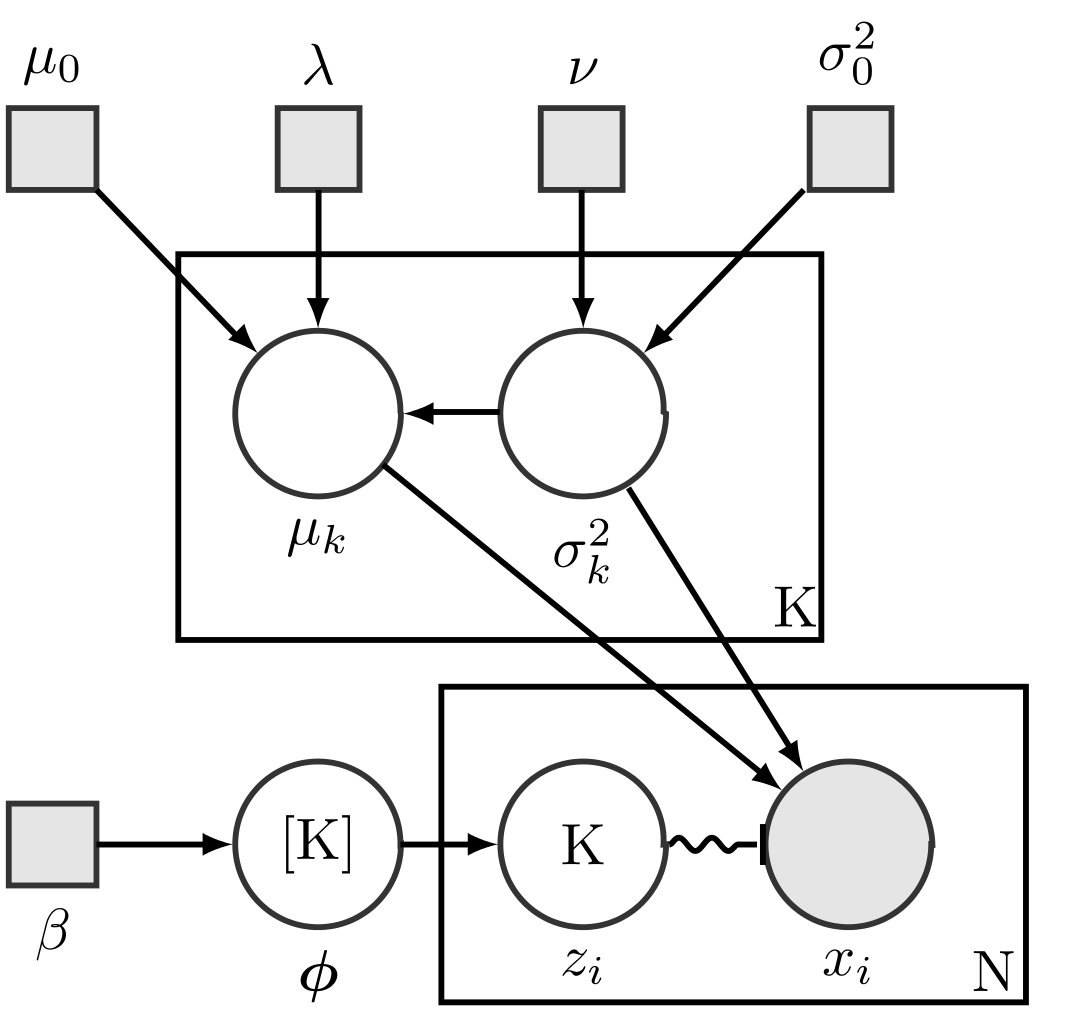
\includegraphics[height=8cm]{background/Figures/BGMM.png}
\caption{\gls{pgm} representing the parametric inference of a Gaussian Mixture, see text for details. Figure by Benwing, license: Creative Commons BY-3.0}
\label{fig:pgmGMM}
\end{center}
\end{figure}

\section{The BHM for the Pleiades DANCe data set}
\label{sect:datamodelling}
Creating a model is a complex task. As previously mentioned, a model is a mathematical representation of the knowledge about a certain phenomenon. Thus, constructing a model demands gathering and arranging the \emph{a priori} knowledge of the phenomenon. However, the model is not a isolated entity, in the sense that having a model alone, besides its pure mathematical interest, is almost useless without a data set into which apply it. The data set and the model conform an entity able to produce knowledge, this entity is the likelihood. For this knowledge to be accurate the likelihood must incorporate the information of the data collection mechanism, particularly if the latter is non-ignorable.

The \emph{a priori} knowledge of the Pleiades cluster together with the description of the data collection mechanism of the \gls{ddr2} data set are summarised in Chapter \ref{chap:pleiades}. Here, I describe how this information is assembled to create the \gls{bhm}.

Once the \emph{a priori} knowledge has bee gathered, the creation of the model becomes an iterative and continuous process. Assembling the knowledge into a coherent system demands continuous iterations of decision making, test, and analysis of preliminary results. This Section provides a snapshot of this process: the state of the model once the article \citet{Olivares2017} was submitted.

The following is a brief description of the \gls{bhm}. Probabilistic models (likelihoods) are created for the field and cluster populations. These models, together with the data set, are used to infer both the posterior distributions of the cluster parameters, and the cluster membership probabilities of objects in the data set. Both cluster and field models are assumed to be independent in photometry and proper motions. The proper motions and photometric elements of the field model are described using \glspl{gmm}. The cluster population is additionally model as the joint population of single stars and \gls{emb}. Both cluster proper motions models, for singles and \gls{emb}, are described using \gls{gmm}. The photometric models of both single and \gls{emb} consist of multivariate normal distributions whose means and covariances are parameters of the model. The means of these multivariate normal distributions are parameterised by means of spline functions. In turn, these are parametrised by the \emph{true} \gls{ci} of each star, which is marginalised using the \emph{true} colour distribution. Later, this \emph{true} \gls{ci} distribution will be used, in combination with the splines parameters, to derive the distributions of the magnitudes, and from them the luminosity distributions. 

The details are explained in the following Sections. First, Section \ref{sect:missing}, explains the statistical procedure to deal with one of the crucial aspects of the \gls{ddr2} data set: the missing information. Later, Section \ref{sect:generative-model} provides details of how the relevant knowledge about the Pleiades cluster and field populations are embedded in the generative model of the data. Finally, Sections \ref{sect:field_population} and \ref{subsect:cluster} deal with the explanation of the field and cluster model, respectively.

\subsection{Treatment of missing information}
\label{sect:missing}

Missing information refers to at least two forms of absent values. In one hand, there are the data completely lost and from which the data set contains no information at all (except perhaps for the number of lost objects). On the other hand, there are the data that has been partially observed, and thus contains missing entries in some of its observables, but not in all of them.

A missing entry or missing value refers to a non-measured or non-available value in the vector of measurements of an object. It can arise due to different statistical or physical processes. 

From the physical perspective, missing values occur due to faint or bright sources that produce counts values outside the dynamical range of the detector. They can also emerge due to detector malfunctions (e.g. electronic failures), or to random effects (e.g. cosmic rays).

From the statistical perspective, it is important to know if the origin of the missing information, called the missing process, is deterministic or stochastic. In the former, they occur only above or below a certain hard limit, while in the latter, they follow a probability distribution. If its origin is deterministic, there are two possible scenarios: censoring and truncation. 

Truncation occurs when the data set contains measures of the population but until a certain limit. All information of the population above this limit is lost. Thus, the data set does not contain records, neither of the measured value nor of the number of measurements, for objects whose measured quantity lies outside the truncation limits.  On the other hand, censoring happens when the data set contains only partial information about the actual value of the measured quantity. This information is the number of objects with missing values and the threshold limit upon which they appear. Basically, censoring happens when the value lies outside the upper or lower limits of the measuring instrument, and the number of these objects become the only available record.

In the \gls{ddr2}, the proper motions are truncated to lay within the limits of -100 mas yr$^{-1}$ and 100 mas yr$^{-1}$ in both R.A. and Dec., see Section \ref{sect:DR2}. However, due to its heterogenous origin, it does not posses unique truncation or censoring limits in its photometry.  Although these limits could also be inferred from the data, the large number of \gls{ddr2} sources (not just surveys, but instruments and detectors) prohibits this task. 

To account for the missing information the likelihood of the data must be modified. In truncation, the likelihood is renormalised to integrate to one within the observed limits, while in censoring this renormalisation account for the number of censored data. However, if the missing process is stochastic a more detailed treatment is needed. 

However, in the \gls{ddr2} missing values not only occur because of censoring or truncation.  Other sources of missing values include but are not restricted to cosmic rays, hot pixels, halos of bright stars, diffraction patterns and cross-matching failures. The statistical treatment of missing values originating from each of these sources lies beyond the scope of this work. 

In terms of probability, there is no distinction between missing values and parameters. Therefore, when computing the likelihood $p(\mathbf{d}|\boldsymbol{\theta})$, where $\mathbf{d}$ is the datum with a missing entry, and $\boldsymbol{\theta}$ is the set of likelihood parameters, we can marginalise the missing values as we do with any other nuisance parameter: with the aid of a prior. In this case, the prior sets the probability of finding a missing value within the domain of the observable. This prior probability can also be conditioned on extra information that may or not be available. For example, it can be conditioned on other observations (usually called covariates, e.g. the proper motions or sky positions), in the value of the observed (non-missing) entries $\mathbf{d}_{obs}$, or in parameters of the missing data collection mechanism, which can also be inferred from the data in hierarchical fashion.

The interested reader can find, in Chapter 8 of \citet{Gelman2013}, a detailed description of the variety of schemes to account for the data collection mechanism, including the special cases of censoring and truncation. In general, the missing data mechanism can be accounted for by expressing the missing values entries with index $I$ (a matrix of dimensions equal to those of the data, with ones in the entries corresponding to the observed entries in the data and zeros in the missing ones) and modifying the likelihood to account for the missing information.

The likelihood of the complete datum, which comprises not just the observed and missing datum $\mathbf{d}=\{\mathbf{d}_{obs},\mathbf{d}_{mis}\}$, but also the index $I$, conditioned on the model parameters $\boldsymbol{\theta}$, is

\begin{align}
p(\mathbf{d},I|\boldsymbol{\theta})&=p(I|\mathbf{d},\boldsymbol{\theta})\cdot p(\mathbf{d}|\boldsymbol{\theta}), \nonumber
\end{align}
with $p(I|\mathbf{d},\boldsymbol{\theta})$ the missingness probability.

However, the actual information available in the datum is $(\mathbf{d}_{obs},I)$. Thus, the observed-datum likelihood can be expressed as
\begin{equation}
\label{eq:marginalmis}
p(\mathbf{d}_{obs},I|\boldsymbol{\theta})=\int p(\mathbf{d}|\boldsymbol{\theta})p(I|\mathbf{d},\boldsymbol{\theta})\mathrm{d}\mathbf{d}_{mis},
\end{equation}
where the missing values have been marginalised with the aid the prior $p(I|\mathbf{d},\boldsymbol{\theta})$. 

The probability $p(I|\mathbf{d})$ can be assumed to be uniform, which results in what is called the \emph{ignorability} of the data collection mechanism. The result of this assumption is that $p(\mathbf{d}_{obs},I|\boldsymbol{\theta})= p(\mathbf{d}_{obs}|\boldsymbol{\theta})$, which is equivalent to ignore the missing mechanism. This assumption is incorrect because, as shown in Section \ref{sect:DR2}, missing values are most probable at the faint photometric ends.

The probability $p(I|\mathbf{d},\boldsymbol{\theta})$ is formally not known because \gls{ddr2} is a compilation of data from a variety of surveys. Thus the data collection mechanism is neither homogeneous nor totally understood\footnote{ The DANCe team is currently working on the assessing of the missingness process. In particular, we are interested in the detection probability as a function of signal-to-noise and sky position. The latter is of paramount importance in the vicinity of bright sources where halos and artefacts have the largest impact.}. In spite of that, it can also be assumed that the collection mechanism depends only on the observed values, $\mathbf{d}_{obs}$. Such assumption is called \emph{missing at random} \cite[][p. 450]{Gelman2013} because the distribution of the missing-data mechanism does not depend on the missing values. This assumption is still incorrect because, as shown in Section \ref{sect:DR2},  the probability of detecting an object depends on its brightness. However, under this assumption, $p(I|\mathbf{d},\boldsymbol{\theta})=p(I|\mathbf{d}_{obs})$. Thus, Equation \ref{eq:marginalmis} reduces to,

\begin{align}
\label{eq:MAR}
p(\mathbf{d}_{obs},I|\boldsymbol{\theta})&=\int p(\mathbf{d}|\boldsymbol{\theta})\cdot p(I|\mathbf{d}_{obs})\mathrm{d}\mathbf{d}_{mis}\nonumber \\
&=p(I|\mathbf{d}_{obs})\cdot \int p(\mathbf{d}_{mis},\mathbf{d}_{obs},|\boldsymbol{\theta})\mathrm{d}\mathbf{d}_{mis}\nonumber\\
&=p(I|\mathbf{d}_{obs})\cdot p(\mathbf{d}_{obs}|\boldsymbol{\theta}).
\end{align}

This approach is similar to the use of the so called \emph{selection function} \cite[see for example][]{2013SADM....6...15A}. Indeed, the probability $p(I|\mathbf{d}_{obs})$, is the probability of including the object with observables $\mathbf{d}_{obs}$ in the data set under analysis. Thus we can call it  \emph{selection probability}.

As kindly suggested by Stefano Andreon (one of the referees of this work), another possibility to compute the likelihood function based on the observed data is given by Equation 30 of \citet{2013SADM....6...15A}. In the latter,

\begin{equation}
\label{eq:selectionfunction}
p(y_i^{obs}|I_i = 1,y_i,\theta)=\frac{f(I_i=1|y_i)\cdot p(y_i^{obs}|y_i,\theta)}{\int f(I_i=1|z)\cdot p(z|y_i,\theta),\mathrm{d}z}
\end{equation}

where $y_i$ and $y_i^{obs}$ are the true and observed values, respectively, $f(I_i=1|y_i)$ is the \emph{selection function}, and $p(y_i^{obs}|y_i,\theta)$ is the likelihood of the observed data given the true data and the parameters $\theta$. 

However, in the \gls{bhm} the previous approach can not be used because of the following reasons. First, the \gls{rdr2} has a \emph{selection function} which is almost impossible to estimate given that objects are selected based on their membership probability to the cluster. Even if a simpler selection function could be used instead (like cuts in the observable space), the resulting one will be the \emph{selection function} conditioned on the observed values, and not in the true ones, as required by Eq. \ref{eq:selectionfunction}. Furthermore, this approach is computationally expensive due to the integral in the denominator of Eq. \ref{eq:selectionfunction}, and using it will result in an even larger computing time.

As it will be shown in the next section, the likelihood of the data (Eq. \ref{eq:marginalmis}) will be partitioned in the likelihoods of the cluster and field (Eq. \ref{eq:genmod}). Since the objects in the \gls{rdr2} were selected based on their cluster membership probability, then, under the assumption of \emph{missing at random}, the cluster \emph{selection probability} is $p(I|\mathbf{d}_{obs})=1 - 10^{-11}$, where $10^{-11}$ is the probability of leaving one cluster member out of the \gls{rdr2} (see Section \ref{sect:RDR2}). Therefore, we can safely assume that the cluster \emph{selection probability} is one. Thus from Eq. \ref{eq:MAR}, $p(\mathbf{d}_{obs},I|\boldsymbol{\theta})=p(\mathbf{d}_{obs}|\boldsymbol{\theta})$.



Summarising, in the treatment of missing values I make the following assumptions.

\begin{itemize}
\item The cluster data collection mechanism is \emph{missing at random} with \emph{selection probability} $p(I|\mathbf{d}_{obs})=1$.
\item The field data collection mechanism is \emph{ignorable} with $p(I|\mathbf{d})$  uniform.
\end{itemize}

This assumptions, although incorrect, are taken because of the following reasons. 

First, the $p(I|\mathbf{d},\boldsymbol{\theta})$ for the formal treatment of missing values in Eq. \ref{eq:marginalmis} is not known.

Second, even if the probability $p(I|\mathbf{d},\boldsymbol{\theta})$ would be available (or an approximation of it), the current computational capabilities will not allow to numerically evaluate the integral of Eq. \ref{eq:marginalmis}. The use of a uniform probability enable us to analytically evaluate this integral thus avoiding the high computational burden of computing it for each object and missing value in the data set and at each step in the MCMC chain.

Therefore, although the \emph{ignorability} assumption is not correct, it currently provides the simplest and straight forward option to perform the expensive integral of Eq. \ref{eq:marginalmis}. Since this assumption is incorrect, and therefore results in biased estimators of the true population parameters, in the following section I quantify this biases.

\subsubsection{Validity of the \emph{ignorability} assumption.}
\label{sect:ignorability}

In this Section, I present the quantification of the bias introduced by assuming the \emph{ignorability} of the missing mechanism. In addition, I also quantify the bias introduced by assuming that the true population parameters can be recovered using only completely observed objects and discarding those with missing entries. The latter, which here I call the \emph{naivety} assumption, is common practice in the literature (at least in the works mentioned in Section \ref{sect:current_methodologies}. Notice that these two assumptions, \emph{naivety} and \emph{ignorability} are undistinguishable in the absence of correlations amongst observables. Therefore, the bias must be quantified in a data set with similar correlations to those in the \gls{rdr2}.

To quantify the biases rendered by these assumptions, I proceed as follows.

First, I assume to know the parameter values of the true population. Thus, I use the parameter values of the \gls{gmm} describing the photometry of the field population contained in the \gls{rdr2} data set. In specific, I assume that these true parameter values are those inferred in Section \ref{sect:field_population}. 

Second, using these true parameter values I generate a synthetic data set with $10^4$ objects.

Third, using the real data from the \gls{rdr2}, I mask as missing entries the photometric entries in the synthetic data. The masking procedure is the following.

Given that the $K_s$ photometric band is the most observed one in the \gls{rdr2}, I use it as covariate, and to obtain the probability of having a missing value. Thus,
\begin{equation}
p(I_x=0 | K_s)=\frac{p(K_s|I_x = 0)\cdot p(I_x=0)}{p(K_s)},\nonumber
\end{equation}
where $I_x=0$ stands for the probability that the photometric band $x$ which can be $\{i-K_s,Y,J,H\}$ is missing, $p(K_s|I_x = 0)$ is the probability of $K_s$ given that the band $x$ is missing, $p(K_s)$ is the probability of all observed values of $K_s$, and $p(I_x=0)$ is the fraction of objects with missing entries in the $x$ band. Then, I create a synthetic random matrix $R$ of size equal to that of the synthetic data. The entries in this matrix are drawn from a uniform probability distribution between zero and one. Then, objects in the synthetic data set are masked as missing if and only if 
\begin{equation}
\label{eq:mask_missing}
 \left\{ \begin{array}{rcl}
       R_{i,x} > p(I_x=0 | K_s) & \mbox{for} & x\in \{i-K_s,Y,J,H\} \\ 
       R_{i,x} > p(I_x=0 ) & \mbox{for} & x =K_s 
\end{array}\right.
\end{equation}
with $p(I_{K_s}=0 )$ the fraction of objects with missing values in $K_s$. The latter assumes that missing values in $K_s$ are uniformly distributed.

Thus, I now have three synthetic data sets. The original one, with completely observed entries (hereafter Complete), the one with missing values (hereafter Missing), and, the one resulting from taking only the completely observed objects from the one with missing values (hereafter Observed). Figure \ref{fig:ignorability_synthetic} shows the distribution of objects in these data sets as a function of the photometric magnitude for each magnitude. To each of these data sets, I apply the \gls{gmm} algorithm (the one described in Section \ref{sec:codeGMM}) and recover the fractions, means and covariance matrices of the \gls{gmm}. I call these set of parameters and the densities they produce Complete, Missing, and Observed, in accordance to the data set from which they were obtained.

\begin{figure}[ht!]
    \centering
    \begin{subfigure}[t]{0.45\textwidth}
        \includegraphics[page=2,height=6cm]{background/Figures/Check_distributions.pdf}
    \end{subfigure}
    \begin{subfigure}[t]{0.45\textwidth}
      \includegraphics[page=3,height=6cm]{background/Figures/Check_distributions.pdf}
    \end{subfigure}
     \begin{subfigure}[t]{0.45\textwidth}
      \includegraphics[page=4,height=6cm]{background/Figures/Check_distributions.pdf}
    \end{subfigure}
     \begin{subfigure}[t]{0.45\textwidth}
      \includegraphics[page=5,height=6cm]{background/Figures/Check_distributions.pdf}
    \end{subfigure}
\caption{Density distributions in $Y,J,H$ and $K_s$ bands of the synthetic objects in the Complete, Missing and, Observed data sets. See text.}
\label{fig:ignorability_synthetic}
\end{figure}

By means of these three set of parameters, I can quantify the bias induced by the \emph{ignorability} and \emph{naivety} assumptions. The first is given by the Missing data set and parameters, while the later by the Observed data set and parameters. Furthermore, to minimise the effects of the sample size in the comparisons, instead of comparing the Missing and Observed set of parameters to the true parameters, I  use the Complete set of parameters. 

I quantify differences by means of the Root Mean Square Deviation, which is defined as, 

\begin{equation}
RMSD = \sqrt{\frac{\sum_i^n(\frac{x_i-y_i}{y_i})^2}{n}}, \nonumber
\end{equation}

where $x_i$ is the density given by the Missing or Observed \glspl{gmm} and $y_i$ is the density given by the Complete \gls{gmm}. 

The densities of the Complete, Missing and Observed \glspl{gmm} are evaluated in grids (with $n$ total points separated by 0.05 mag) in each of the $Y,J,H,K_s$ vs \gls{ci} \glspl{cmd}. The RMSDs are computed just for those points in the grids where the Complete density is higher than $10^{-3}$, which avoids the regions far from the cluster sequence where the density vanishes. Figure \ref{fig:ignorable_and_naive} shows the RMSDs of the Missing and Observed \glspl{gmm} compared to the Complete one. As can be seen, the Observed parameters return projected densities that are over-estimated in the central parts, particularly at $\gls{ci}\sim3.5$. On the other hand, the Missing parameters return densities similar to the original ones across the \gls{cmd}.

The mean RMSD of the Observed  and Missing \glspl{gmm} in the four \glspl{cmd} are $0.78\pm0.38$ and $0.21\pm0.4$, respectively. Uncertainties are the standard deviation of the four RMSDs.

\begin{figure}[ht!]
\begin{center}
\begin{subfigure}[t]{0.45\textwidth}
\includegraphics[page=2,width=\textwidth]{./background/Figures/validationMissing.pdf}
\end{subfigure}
\begin{subfigure}[t]{0.45\textwidth}
\includegraphics[page=4,width=\textwidth]{./background/Figures/validationMissing.pdf}
\end{subfigure}
\begin{subfigure}[t]{0.45\textwidth}
\includegraphics[page=6,width=\textwidth]{./background/Figures/validationMissing.pdf}
\end{subfigure}
\begin{subfigure}[t]{0.45\textwidth}
\includegraphics[page=8,width=\textwidth]{./background/Figures/validationMissing.pdf}
\end{subfigure}
\caption{Contours comparing the relative deviations of the Observed (left panels) and Missing (right panels) \glspl{gmm} when compared to the Complete \gls{gmm} (in grey scale at the background), projected in each of the \glspl{cmd} used in this work.  Regions where the density of the Complete model goes below $10^{-3}$ are not shown.}
\label{fig:ignorable_and_naive}
\end{center}
\end{figure}

In addition, the mean absolute relative difference of the Missing and Observed set of parameters when compared to the Complete ones are $0.42 \pm 2.5$ and $1.5 \pm 3.2$, respectively.  

The previous values indicate that the Missing and Observed \gls{gmm} resulting from the \emph{ignorability} and \emph{naivety} assumptions, respectively are indeed biased. However, as this figures demonstrate, the bias introduced by the \emph{naivety} assumption is more than 3.5 times larger than that introduced by the \emph{ignorability} assumption. Furthermore, the \emph{naivety} reaches its maximum deviation at \gls{ci}= 3.5, exactly where the cluster reaches is peak density, which is not a coincidence. The cluster members have been thoroughly observed.

In spite of the incorrectness of the \emph{ignorability} assumption, which nevertheless enable us to analytically perform the marginalisation integral (Eq. \ref{eq:marginalmis}) and reduce the computing time, it renders better estimates of the true population parameters than the commonly spread naivety assumption used by the previous works from the literature (see Section \ref{sect:current_methodologies}). 

\subsection{The generative model}
\label{sect:generative-model}
In the \gls{ddr2} data set, cluster stars and field sources are mixed. Their probabilistic disentanglement requires probabilistic models for each population, i.e. their likelihoods. The true values of these two likelihoods, field and cluster, will be given given by parametric relations embodying the state of knowledge of \gls{nyc} (i.e. the models of cluster and field).  Using these likelihoods, the individual cluster membership probability of each object in the data set is computed (by means of Eq. \ref{eq:prob}). These \glspl{pdf}  together with a probability classification threshold, allow individual objects to be separated into cluster and field populations.

The inference process demands a set of $N$ binary integers $\mathbf{q}$, one $q_n$ for each object. The two possible values of these binary integers represent one of the two mutually exclusive possibilities: the object belongs to the cluster ($q_n=1$) or to the field population ($q_n=0$). 

Let $\boldsymbol{\theta}$ and $\boldsymbol{\phi}$ be the parameters of the cluster and field models, and $p_c$ and $p_f$ their likelihoods, respectively. Then, the likelihood of the data, $\mathbf{D}$, is,

\begin{equation}
p(\mathbf{D}|\mathbf{q},\boldsymbol{\theta},\boldsymbol{\phi})= \prod_{n=1}^N {p_c(\mathbf{d}_n|\boldsymbol{\theta})}^{q_n}\cdot {p_f(\mathbf{d}_n|\boldsymbol{\phi})}^{(1-q_n)}.
\end{equation}

The inference of these $N$ binary integers will demand a computing power that is outside the current possibilities. Thus, instead of inferring them, I marginalise them using a prior probability, which is set in terms of a new and unique parameter $\pi$. It represents the \emph{prior} probability that an object belongs to the field. Thus, the prior probability of $\mathbf{q}$ is

\begin{equation}
p(\mathbf{q}|\pi)= \prod_{n=1}^N {(1-\pi)}^{q_n}\cdot {\pi}^{(1-q_n)}.
\end{equation}

Since the entries in $\mathbf{q}$ can only take as value zero or one, the marginalisation integral is indeed a sum. Furthermore, the domain of this sum is the $2^N$ possible ways to combine the binary variables $q_n$. Thus, the marginalisation sum over all these $2^N$ possible states results in,

\begin{align}
p(\mathbf{D}|\pi,\boldsymbol{\theta},\phi)&=\sum_{\mathbf{q}} p(\mathbf{D},\mathbf{q}|\pi,\boldsymbol{\theta},\phi)\nonumber\\
&=\sum_{\mathbf{q}} p(\mathbf{D}|\mathbf{q},\pi,\boldsymbol{\theta},\phi)\cdot p(\mathbf{q}|\pi) \nonumber \\
&=\sum_{\mathbf{q}} \prod_{n=1}^N {p_c(\mathbf{d}_n|\boldsymbol{\theta})}^{q_n}\cdot {p_f(\mathbf{d}_n|\phi)}^{(1-q_n)}\cdot \prod_{n=1}^N {(1-\pi)}^{q_n}\cdot {\pi}^{(1-q_n)} \nonumber \\
&=\sum_{\mathbf{q}} \prod_{n=1}^N \left[(1-\pi)\cdot p_c(\mathbf{d}_n|\boldsymbol{\theta})\right]^{q_n}\cdot \left[\pi\cdot p_f(\mathbf{d}_n|\phi)\right]^{(1-q_n)} \nonumber \\
&=\prod_{n=1}^N (1-\pi)\cdot p_c(\mathbf{d}_n|\boldsymbol{\theta}) + \pi\cdot p_f(\mathbf{d}_n|\phi).
\end{align}
This last equality is a rather complicated derivation which can be found in \citet{Press1997}, and in \citet{Hogg2010a} for $p_c$ and $p_f$ in the exponential family. Also, a general derivation of this expression is given by \citet{Jaynes2003}. He obtains it assuming individual unknown probabilities $p_n$ instead of $q_n$ and marginalising over them with the aid of a prior.

Thus, the \emph{generative model} or likelihood of the datum $\mathbf{d_n}$  is

\begin{equation}
\label{eq:genmod}
p(\mathbf{d}_n | \pi,\boldsymbol{\theta}_c,\boldsymbol{\theta}_f,\mathbf{u}_n)=\pi \cdot p_f(\mathbf{d}_n|\boldsymbol{\theta}_f,\mathbf{u}_n) + (1-\pi)\cdot p_c(\mathbf{d}_n| \boldsymbol{\theta}_c,\mathbf{u}_n),
\end{equation}

where $\boldsymbol{\theta}_f$ and $\boldsymbol{\theta}_c$ indicate the cluster and field parameters, while $\mathbf{u}_n$ refers to the datum uncertainty. The probabilities $p_f(\mathbf{d}_n|\boldsymbol{\theta}_f,\mathbf{u}_n)$ and $p_c(\mathbf{d}_n| \boldsymbol{\theta}_c,\mathbf{u}_n)$ are the field and cluster models, respectively. These models are explained in detail in the next two sections.

The cluster membership probability of each object in our data set are computed from the elements in Eq. \ref{eq:genmod}, by means of Eq. \ref{eq:prob}. Thus, the cluster membership probability is given by,

\begin{equation}
\label{eq:prob_dist}
p( \mathcal{M}_c | \mathbf{d}_n) =\frac{p_c(\mathbf{d}_n| \boldsymbol{\theta}_c,\mathbf{u}_n)\cdot (1-\pi)}{\pi \cdot p_f(\mathbf{d}_n|\boldsymbol{\theta}_f,\mathbf{u}_n) + (1-\pi)\cdot p_c(\mathbf{d}_n| \boldsymbol{\theta}_c,\mathbf{u}_n)},
\end{equation}
In Eq. \ref{eq:prob}, the probabilities $P( \mathcal{M}_k | \mathbf{d})$ are \gls{pmf} because the probabilities $P( \mathcal{M}_k )$ are themselves \gls{pmf}. However, in Eq. \ref{eq:prob_dist}, by setting the prior probability $\pi$ as a random variable ($\pi \in [0,1]$), which is itself inferred from the data in a hierarchical way and with prior \gls{pdf} given by a Dirichlet distribution $Dir(\boldsymbol{\alpha})$ (with $\boldsymbol{\alpha}$ its hyper-parameter), then $p(\mathcal{M}_c | \mathbf{d}_n)$ also follows a probability distribution. To demonstrate this, let 
\begin{align}
y&= p( \mathcal{M}_c | \mathbf{d}_n),\nonumber \\
g(\pi)&= \frac{p_c(\mathbf{d}_n| \boldsymbol{\theta}_c,\mathbf{u}_n)\cdot (1-\pi)}{\pi \cdot p_f(\mathbf{d}_n|\boldsymbol{\theta}_f,\mathbf{u}_n) + (1-\pi)\cdot p_c(\mathbf{d}_n| \boldsymbol{\theta}_c,\mathbf{u}_n)},\nonumber \\
\pi &\sim p(\pi),\nonumber
\end{align}
with $p(\pi)$ the probability distribution of the random variable $\pi$, and $g(\pi)$ a linear transformation of $\pi$.
Then, by definition $y \equiv g(\pi)$, and $y$ follows the probability distribution given by $y= g(p(\pi))$. Since the parameter $\pi$ is also inferred from the data, then each cluster membership probability determined in this work is itself a \gls{pdf}. 



In the following, I assume that the observed quantities result from the convolution of the model likelihood, given the \emph{true} quantities, with the uncertainty process (see Section \ref{sect:parametric_inference}). The latter could be different for each object, thus resulting in different individual uncertainties. Thus, the model allows heteroscedatic uncertainties. Although these uncertainties are not assumed to have the same values, I assume that tall of them are multivariate normal.  This assumption is standard practice and is also supported by the large and heterogeneous origins of the \gls{ddr2} data set. 

\subsection{The field population}
\label{sect:field_population}
To model the field population, I assume that the joint seven-dimensional probability distribution of the field can be factorised into the probability distributions of proper motions and photometry. Thus, the field likelihood of the proper motions and the photometry are assumed to be independent. Also, I assume that both distributions are described by \gls{gmm}. The flexibility of \glspl{gmm} to fit a variety of distribution geometries makes them a suitable model to describe the field density of the heterogeneous \gls{ddr2} data set. 

A \gls{gmm} is a probability distribution resulting from the linear combination of $M$ Gaussian distributions, 
\begin{equation}
p_{GMM}(x|\boldsymbol{\pi},\boldsymbol{\mu},\boldsymbol{\Sigma})=\sum_{m=1}^M \pi_m \cdot \mathcal{N}(\boldsymbol{\mu}_m,\boldsymbol{\Sigma}_m),
\end{equation}
{where $\pi_m$ is the fraction of the $m$th Gaussian, $\boldsymbol{\mu}_m$ its mean and, $\boldsymbol{\Sigma}_m$ its covariance matrix. The $m$ fractions must add to one. }

{Notice that the number of Gaussians in the mixture is not formally speaking a parameter, but rather it implies a collection of parameters. The number of these parameters increases linearly with the number of Gaussians and quadratically with the dimension.} 

According to \citet{Bouy2015}, the number of Pleiades candidate members in the \gls{ddr2} data set is 2010 (going up to 2109 in the combined Tycho+\gls{ddr2}) from a total of 1,972,245 sources. It means that the number of field objects dominates (99.9\%) the \gls{ddr2} data set. Even in our restricted $10^5$ objects data set, \gls{rdr2} (see Sect. \ref{sect:RDR2}), the field still dominates with a 0.98 fraction. Thus, it can be assumed that any classification of candidate members will have a negligible impact on this figure. Therefore, it seems reasonable to assume that the \gls{gmm} describing the field population can be frozen (fixed) during the process of cluster parameters inference. I elaborate more on this assumption.


The objects that \citet{Bouy2015} classified as belonging to the field are those whose cluster membership probabilities are lower than 0.75. This probability threshold corresponds to the one found by \citet{Sarro2014} after analysing the performance of their methodology when applied to synthetic data sets. In \citet{Sarro2014} the authors report that, at a probability threshold $p=0.75$, the contamination and true positive rates are $\sim 8\%$ and $ \sim96\%$ respectively. Assuming that these values are correct, the real number of field objects would change by approximately 4\% of the cluster members (adding the 8\% of contaminants and subtracting the 4\% of missed members), thus $\sim 80$ objects. This value is negligible compared to the size of the data set ($10^5$ objects in the \gls{rdr2}). It represents the negligible fraction of $ 8\times10^{-4}$. 

It can be further assumed that these hypothetically misclassified objects are spread in the space of observables. Indeed, these misclassified objects can be thought to have membership probabilities near the classification threshold. Thus, they may lay in the entanglement regions which corresponds, in proper motions, to a halo around the cluster centre, and in photometry, to a region around the cluster sequence. For example, these objects could have photometry that agrees with the cluster sequence but proper motions that are far from it. There are several combinations of observables values which may render these intermediate membership probabilities. The observable regions that these objects may populate allows us to assume that they are spread over the observable space. 

%Furthermore, under the assumption that the work of \citet{Sarro2014} is correct, the misclassified objects concentrate on cluster membership probabilities near the classification threshold. Therefore, they will also group in an area of the physical "boundary" between the cluster and the field (I call it physical because it is on the observable variables and not in the probability threshold). This is the area of highest entanglement. It does not mean that misclassified objects will not lie in the core of the cluster (objects with high membership probabilities). It means that the occurrence of these cases will be lower.  This physical "boundary" will correspond, in proper motions space to a halo around the cluster centre. In photometry, however, this boundary will run all along the cluster sequence in the CMDs. All previous assumptions are there to justify that the negligible fraction of hypothetical misclassified  objects is not concentrated in the physical space. 

If the misclassified objects are a few and spread over the observable space, then their contribution to the parameters of the \gls{gmm} describing the field population can be neglected. Thus, the parameters of the \gls{gmm} can remain fixed and out of the inference process. 

The previous assumption is of paramount importance due to practical reasons, but because the field parameters remain fixed, their uncertainty is not propagated to cluster parameters an neither to membership probabilities. If I were to simultaneously infer the parameters of both cluster and field models, even only those of the field proper motions \gls{gmm}, the required computing time would be excessive. The number of parameters in the field \gls{gmm} goes up to $\sim 300$, more than twice that of the cluster model (85 parameters). {Even inferring only the 42 parameters of the field proper motions \gls{gmm} would represent, at least, a 50\% increase in the computing time}. Instead, I first fit the parameters of the field \gls{gmm} using the field objects in the \gls{rdr2} (the $\sim 98,000$ objects with membership probabilities below 0.75) and then I keep these parameters fixed in the inference process.   

 

The number of gaussians for the proper motions and photometric \gls{gmm} is found using the \gls{bic} introduced by \citet{Schwarz1978}. The \gls{bic} is a model selection criterium that aims at avoiding over-fitting. It represents a compromise between the likelihood, $\mathcal{L}$, of the $n$ data points, and the number of parameters, $k$. This is,

\begin{equation}
\label{eq:BIC}
BIC = \ln{n}\cdot k - 2 \ln{\mathcal{L}}.
\end{equation}

To estimate the parameters of the \gls{gmm} we use the \gls{em} algorithm. However, the missing values in the photometry prevent the use of the standard form of the algorithm \cite[see for example Chapter 9 of][]{Bishop2006}.
Instead, I estimated these parameters with the modified version of the \gls{em} algorithm for \gls{gmm} found by \citet{McMichael1996} and rediscovered by me (see Section \ref{sec:codeGMM}). On this version, objects with missing values also contribute to the \gls{mle} of the parameters. The distribution of missing values though is also assumed uniform (i.e. it assumes the ignorability of the missing-value process). I applied this algorithm to the five dimensional photometric observables of the 98,010 objects (from the \gls{rdr2}) with membership probabilities below 0.75 according to \citet{Bouy2015}. I tested \glspl{gmm} whose number of components ranged from 1 to 20. The optimal number of components suggested by the \gls{bic} is 14. Figures \ref{fig:fphGMM} and \ref{fig:fphGMM2} show two dimensional projections of the 14 components in the five dimensional \gls{gmm}. It is important to notice that only $\sim$1\% of these 98,010 objects have completely observed photometry (i.e. no missing values in any observable). For this reason, some of the Gaussians appear empty in Fig. \ref{fig:fphGMM}. However, Fig. \ref{fig:fphGMM2} shows projections of the same 14 component and five dimensional \gls{gmm} in the magnitude-magnitude diagrams, where the percentage of completeness is above 80\%. As a consequence, there are no empty Gaussians in this Figure, as shown by the log scale density. If we were to work only with the completely observed objects and discarded 99\% of the data set, our derived parameters would be severely biased (see Section \ref{sect:missing}).

\begin{figure}[ht!]
    \centering
    \begin{subfigure}[t]{0.48\textwidth}
        \includegraphics[page=2,height=8cm,width=\textwidth]{background/Figures/Field_GMM.pdf}
        \caption{}
    \end{subfigure}
    \begin{subfigure}[t]{0.48\textwidth}
      \includegraphics[page=3,height=8cm,width=\textwidth]{background/Figures/Field_GMM.pdf}
        \caption{}
    \end{subfigure}
     \begin{subfigure}[t]{0.48\textwidth}
      \includegraphics[page=4,height=8cm,width=\textwidth]{background/Figures/Field_GMM.pdf}
        \caption{} 
    \end{subfigure}
     \begin{subfigure}[t]{0.48\textwidth}
      \includegraphics[page=5,height=8cm,width=\textwidth]{background/Figures/Field_GMM.pdf}
        \caption{}
    \end{subfigure}
\caption{\glspl{cmd} showing projections of the 14 components in the \gls{gmm} (ellipses for the covariance matrix and crosses for the mean) used in the model the field photometry. The density of field objects with $p <0.75$ \cite[according to][there are 98010 field objects]{Bouy2015} is shown in grey scale. Notice that only $\sim2.4\%$ of these field objects have complete observations in these projections. For this reason, some of the Gaussians appear almost empty. The ellipses shown in Fig. \ref{fig:CMDs_results} represent this \gls{gmm}.}
\label{fig:fphGMM}
\end{figure}

\begin{figure}[ht!]
    \centering
    \begin{subfigure}[t]{0.48\textwidth}
        \includegraphics[page=7,height=8cm,width=\textwidth]{background/Figures/Field_GMM.pdf}
        \caption{}
    \end{subfigure}
    \begin{subfigure}[t]{0.48\textwidth}
      \includegraphics[page=8,height=8cm,width=\textwidth]{background/Figures/Field_GMM.pdf}
        \caption{}
     \end{subfigure}
\caption{Magnitude-magnitude diagrams showing projections of the 14 components in the \gls{gmm} (ellipses and crosses) used in the model the field photometry, and the logarithm of the density (grey) of field objects with $p <0.75$ \cite[according to][there are 98010 field objects]{Bouy2015}. Notice that $\sim85\%$ of these field objects have complete observations in the projections shown.}
\label{fig:fphGMM2}
\end{figure}

In the case of proper motions, since they do not contain missing values, I computed the \gls{gmm} parameters with the standard \gls{em} algorithm. The \gls{bic} finds a model with 15 components, the majority of them with large variances and small fractions (see Fig. \ref{fig:fpmGMM}). These small-fraction Gaussians fit an extended component of the proper motions distributions, which is clearly non-Gaussian. For this reason, we decided modify the mixture of Gaussians by adding a uniform distribution $\mathcal{U}(\mathbf{d}_{pm}|S_{\mu_{\alpha}},S_{\mu_{\delta}})$, with $S_{\mu_{\alpha}}$ and $S_{\mu_{\delta}}$ the support of the proper motions in Right Ascension and Declination, respectively (see Table \ref{tab:DR2properties}). I changed the \gls{em} algorithm to properly account for this modification. The \gls{bic} applied to this new mixture renders more reasonable results (see Fig. \ref{fig:fpmMMM}), with an eight components mixture distribution: seven Gaussians plus the uniform. This modification improves the \gls{gmm} while simultaneously reduces the number of parameters.

\begin{figure}[ht!]
    \centering
    \begin{subfigure}[t]{0.8\textwidth}
        \includegraphics[page=3,width=\textwidth]{background/Figures/GMM-PM-BIC=15.pdf}
        \caption{}
        \label{fig:fpmGMM}
    \end{subfigure}
    \\
    \begin{subfigure}[t]{0.8\textwidth}
      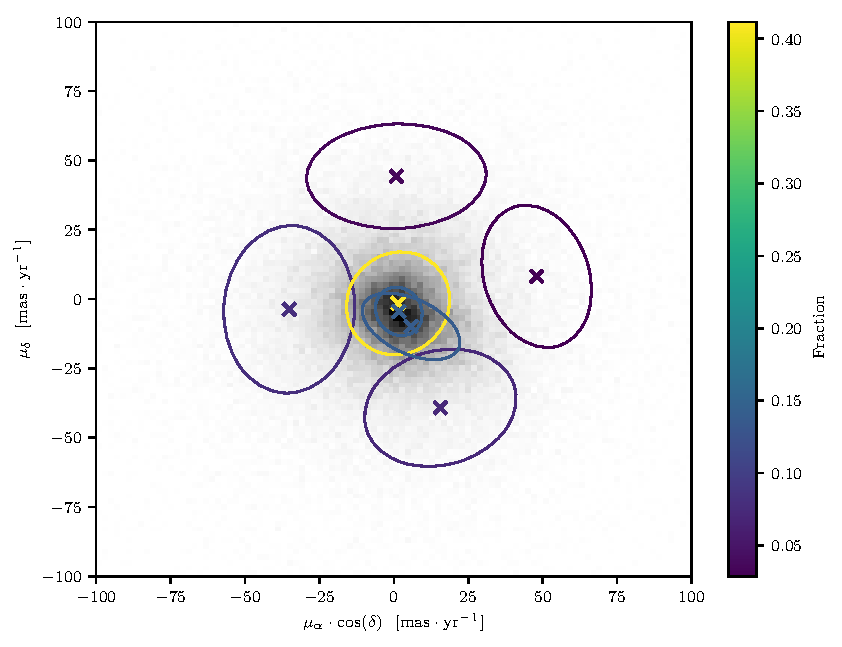
\includegraphics[page=1,width=\textwidth]{background/Figures/Field_GMM.pdf}
        \caption{}
        \label{fig:fpmMMM} 
    \end{subfigure}
\caption{Gaussian (a) and Modified (b) Mixture Models fitted to the proper motions of the field objects in the \gls{rdr2} data set (density in grey scale). The crosses and ellipses indicate the means and the one-$\sigma$ covariance matrices, respectively. The colour code indicates the value of the fraction in the mixture. Uniform distribution not shown in (b). The ellipses in Fig. \ref{fig:PM} show the Modified Mixture Model of this figure.}
\label{fig:GMMvsMMM}
\end{figure}

Finally, the field likelihood $p_f(\mathbf{d}|\boldsymbol{\theta}_f,\mathbf{u})$ of an object with measurements $\mathbf{d}$, given its standard uncertainties $\mathbf{u}$ and the field parameters, $\boldsymbol{\theta}_f$, is
\begin{align}
p_f(\mathbf{d}|\boldsymbol{\theta}_f,\mathbf{u})=&\left[\pi_{f,pm,0}\cdot\mathcal{U}(\mathbf{d}_{pm}|S_{\mu_{\alpha}},S_{\mu_{\delta}})+  \sum \limits_{i=1}^{7}\pi_{f,pm,i}\cdot \mathcal{N}(\mathbf{d}_{pm} | \boldsymbol{\mu}_{f,pm,i},\boldsymbol{\Sigma}_{f,pm,i}+\mathbf{u}_{pm})\right]\cdot  \nonumber \\ 
&\left[ \sum \limits_{i=1}^{14}\pi_{f,ph,i}\cdot \mathcal{N}(\mathbf{d}_{ph} | \boldsymbol{\mu}_{f,ph,i},\boldsymbol{\Sigma}_{f,ph,i}+\mathbf{u}_{ph})\right].
\label{eq:field}
\end{align}
The first and second brackets represent the proper motion (subindex $pm$) and photometric (subindex $ph$) models, respectively, with $\boldsymbol{\pi}_f,\boldsymbol{\mu}_f,\boldsymbol{\Sigma}_f$ their fractions, means and covariance matrices, respectively. The first term of the proper motion model is the uniform distribution, with $\pi_{f,pm,0}$ its fraction. The uncertainty process is convolved (see Section \ref{sect:introprobability}) with the assumed models using the individual proper motions ($\mathbf{u}_{pm}$) and photometric ($\mathbf{u}_{ph}$) uncertainties. 

\textbf{Table \ref{tab:field_parameters} lists the groups (proper motions or photometry), symbols, dimension, and meanings of all the field parameters $\boldsymbol{\theta}_f$ (see Eq. \ref{eq:genmod}) described in this Section. These parameters are derived from the \gls{rdr2} objects whose cluster membership probability is lower than 0.75 according to \citet{Bouy2015}. As stated earlier, these field parameters remain fixed through the inference process of the cluster parameters $\boldsymbol{\theta}_c$ (see Eq. \ref{eq:genmod}). Thus, there is no need to establish priors for them. }

\input{background/Tables/FieldParameters.txt}

\subsection{The cluster population}
\label{subsect:cluster}
Similarly to what I assume for the field population model, I also assume that the cluster model or likelihood can be factorised into the product of the proper motions distribution times the photometric distribution. Thus, I assume these two models are independent. 

It is known that unresolved systems of stars (groups of stars that, given the spatial resolution of the telescope, are seen as an individual object) have an increased brightness proportional to the multiplicity of the system. In particular, if an unresolved system is made of two equally luminous objects, then its magnitude is 0.752 times brighter than that of an individual object. This happens for equal mass binaries.

Since the pioneer work of \citet{Trumpler1921}, we know that some of the Pleiades members are double systems. Recently, \citet{Sarro2014} show evidence that some of these double systems lie in an \gls{emb} sequence. Those authors model the \gls{emb} sequence assuming that its number of objects is 20\% of the total number of cluster members. In the present work, we also model objects is this displaced \gls{emb} sequence  but we do not assume that its proportion is fixed; we infer it from the data. 

Unresolved multiple systems, binary systems particularly, have an impact on the cluster proper motions distribution. In stellar clusters, the massive objects are expected to fall towards the centre of the gravitational potential at a higher rate than that of the less massive ones {\cite[see for example][p. 556]{Binney2008}}. This behaviour arises from stellar encounters in which the energy exchange results in the less massive objects gaining kinetic energy and the massive ones losing it. {Since binaries and multiple systems are typically more massive than the average object, they are expected to fall towards the cluster centre.} From an astrometric point of view, an unresolved system shifts the photo-centre of its images when compared to that of a single object. Given the previous considerations, we decide to model the \gls{emb} as an independent population in the proper motions. Furthermore, we pair this proper motions model to its photometric counterpart. This more comprehensive statistical model allows us to directly compare the kinematic and photometric properties of the \gls{emb} population with those of the rest of the cluster. 

For the sake of simplicity, in the following whenever I refer to the photometric or proper motions model of the \gls{emb}s, I call it the \gls{emb} sequence model (with the subindex $Bs$). I refer to the model of the rest of the stars as the cluster sequence model or simply single stars. Despite that this is an abuse of the terminology, because there are binaries and multiple systems with different mass ratios, it keeps the text more readable.

\subsubsection{Photometric model of single and EMB stars}
\label{sect:cluster_ph}

One of the corner stones of stellar physics is the \gls{hrd} (Fig. \ref{fig:HR}). On it, the luminosity of stars and brown dwarfs is shown against their temperature. As this diagram exhibits, the luminosities and temperatures of stars and brown dwarfs are heavily correlated and occupy very specific loci. Since the beginning of their life, stars and brown dwarfs start to migrate to a narrow sequence called the main sequence, where they live most of their life times. Later (at roughly the ages shown by the green arrows), they start to migrate off the main sequence, and to the regions of giants, supergiants and white dwarfs. The stellar evolution models, like those of \citet{1998A&A...337..403B,2013MmSAI..84.1053A,2014IAUS..299..271A} provide a physical description about how the properties (e.g. temperature, luminosity) of stars and brown dwarfs evolve along their life time.

\begin{figure}[htp!]
\begin{center}
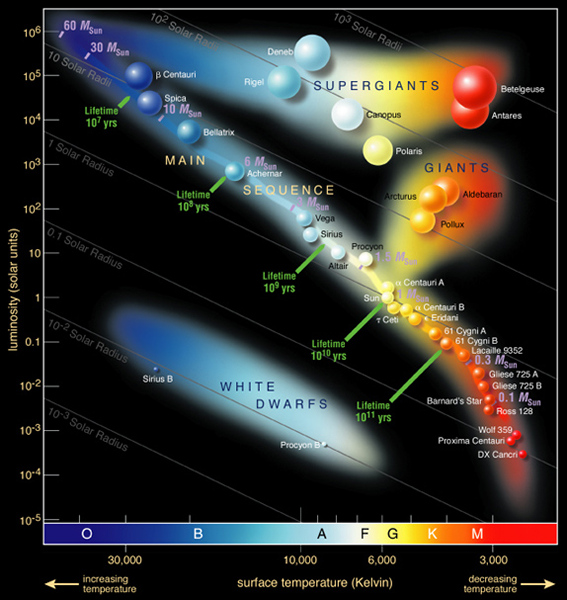
\includegraphics[page=1,width=0.6\textwidth]{background/Figures/Hertzsprung-Russel_StarData.png}
\caption{
Hertzsprung-Russell Diagram identifying many well known stars in the Milky Way galaxy. Image by ESO\url{https://www.eso.org/public/images/eso0728c/}, CC BY 4.0\url{https://commons.wikimedia.org/w/index.php?curid=19915788}
}
\label{fig:HR}
\end{center}
\end{figure}

In star clusters, stars and brown dwarfs are born almost simultaneously (although the birth of the most massive stars might trigger the birth of less massive stars and brown dwarfs), share similar metallicities and are located at similar distances from the observer (assuming that the cluster is smaller compared to the distance to the observer). Thus, the stellar clusters provide the very opportunity to observe, in the space of photometric observables (i.e. apparent magnitudes), the main sequence, which otherwise is blurred by the different ages, metallicities and distances of the objects. Stellar clusters are therefore the very laboratory where the stellar evolutionary models can be tested. Figure \ref{fig:HDRvsCMD} shows the luminosity $L_{\odot}$, in solar units, predicted by the BT-Settl evolutionary models of \citep{2014IAUS..299..271A} for the Pleiades cluster (120 Myr and solar metallically), as function of the effective temperature $T_{eff}$. For comparison, Figure \ref{fig:HDRvsCMD} also shows the $K$ vs. $i-K$ \gls{cmd} of \citet{Bouy2015} Pleiades candidate members. 

\begin{figure}[htp!]
\begin{center}
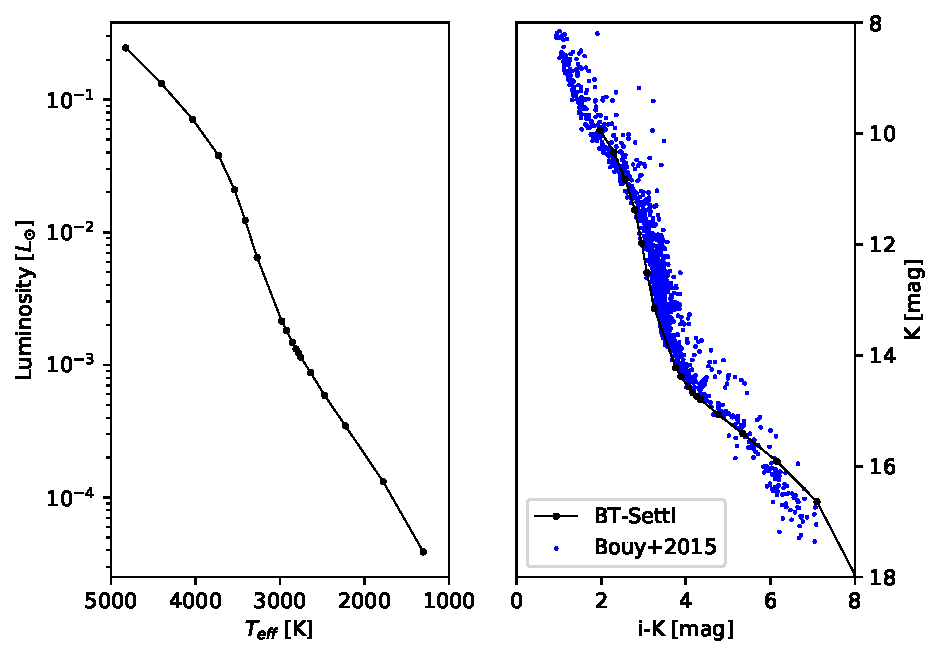
\includegraphics[page=1,width=0.8\textwidth]{background/Figures/Teff_vs_phot.pdf}
\caption{\gls{hrd} (left) $K$ vs. $i-K$ \gls{cmd} (right). The black dots and lines are the Pleiades isochrone given by the BT-Settl models of \citep{2014IAUS..299..271A}. The blue dots are the Pleiades candidate members of \citet{Bouy2015}}
\label{fig:HDRvsCMD}
\end{center}
\end{figure}

Besides the close and almost deterministic relation between the luminosity of stars and brown dwarfs and its effective temperature, the later also determines the bulk of the spectral energy distribution in which the luminosity is emitted. The stars radiative energy is emitted in a distribution of frequencies (or wavelengths) that roughly corresponds to that of a black body (or grey body with emissivity less than one in absorption lines and larger than one in emission lines). The spectral energy distribution of a black body is parametrised by its temperature by means of Planck's law\footnote{
Planck's law describes the amount of radiative energy $B_{\lambda}$, that a body of temperature $T$ gives off at each wave length $\lambda$. Its formulation is 
\begin{equation}
B_\lambda (\lambda,T)=\frac{2hc^2}{\lambda^5}\frac{1}{e^{h c /\lambda k_B T}-1}\nonumber
\end{equation}
where, $h$, $k_B$ and $c$ are Planck's and Boltzmann's constants and the speed of light, respectively. 
}. 

In the ideal model of a star, its luminosity and spectral energy distribution are prescribed by its effective temperature\footnote{The definition of effective temperature is that of a black body that yields the same luminosity per surface area as the star} and radius. 

Because of the previous reasons, the photometric observables can be roughly\footnote{This is a very idealised scenario in which the metallically, variability, magnetic fields, rotation, and other properties have been left aside.} estimated as the combined outcome of the radius and effective temperature of stars and brown dwarfs. Given the importance of the effective temperature, it seems reasonable to find proxies for it in the combination of direct observables. Colour indices are one of these proxies. Defined as the difference of two photometric bands, the provide a proxy for the slope of the spectral energy distribution and therefore for the effective temperature.  However, the quality of the index as an estimator of the effective temperature depends on the latter. 

As mentioned by \citet{1998A&A...333..231B}, the colour index I-K is a good indicator of the effective temperature of M dwarfs. In the light of new theoretical evolutionary models of \citet{2014IAUS..299..271A}, I decided to investigate which of the magnitudes or colour indices available in our set of observables provides the best proxy for the effective temperature. 

Figure \ref{fig:Teff_vs_colours} shows the effective temperature, given by the 120 Myr isochrone of the BT-Settl models \citep{2014IAUS..299..271A}, as a function of the absolute magnitudes and colour indices available in our set of observables. 
As the reader can confirm, given the typical uncertainty of 0.1 mag in the photometric bands, the \glsfirst{ci} provides the best estimator of the effective temperature from within the available colour indices. 


\begin{figure}[htp!]
\begin{center} 
\begin{subfigure}[t]{0.48\textwidth}
\includegraphics[page=2,width=\textwidth]{background/Figures/Teff_vs_phot.pdf}
\end{subfigure}
 \begin{subfigure}[t]{0.48\textwidth}
\includegraphics[page=3,width=\textwidth]{background/Figures/Teff_vs_phot.pdf}
\end{subfigure}
\caption{Effective temperature as a function of the photometric bands and colour indices within the photometric observables of the RF-2 set. Derived from the BT-Settl models \citep{2014IAUS..299..271A} using an age of 120 \gls{myr}.}
\label{fig:Teff_vs_colours}
\end{center}
\end{figure}



Therefore, to model the observed photometric bands, we use function and I choose the \emph{true} \gls{ci} to be the parameter of these functions. As shown in Figures \ref{fig:CI} and \ref{fig:otherCI}, this colour allows the most one-to-one relation with the photometric band $K_s$ (this effect is similar for the rest of the bands). This one-to-one relation, which basically enable us to model the magnitudes as functions of the \gls{ci}, is crucial to avoid degeneracies. Without it, two magnitudes could be described by the same colour index, as it occurs with colour index $J- K_s$ at values $\sim0.9$ (see right panel of Fig. \ref{fig:Teff_vs_colours} and panel b of Fig. \ref{fig:otherCI}). Therefore a simple monotonic relation between colour index and magnitude would not be valid, an injective\footnote{An injective function is a one-to-one function that maps each element in its domain to one and only one in its codomain.} function is needed. 

\begin{figure}[ht!]
\begin{center}
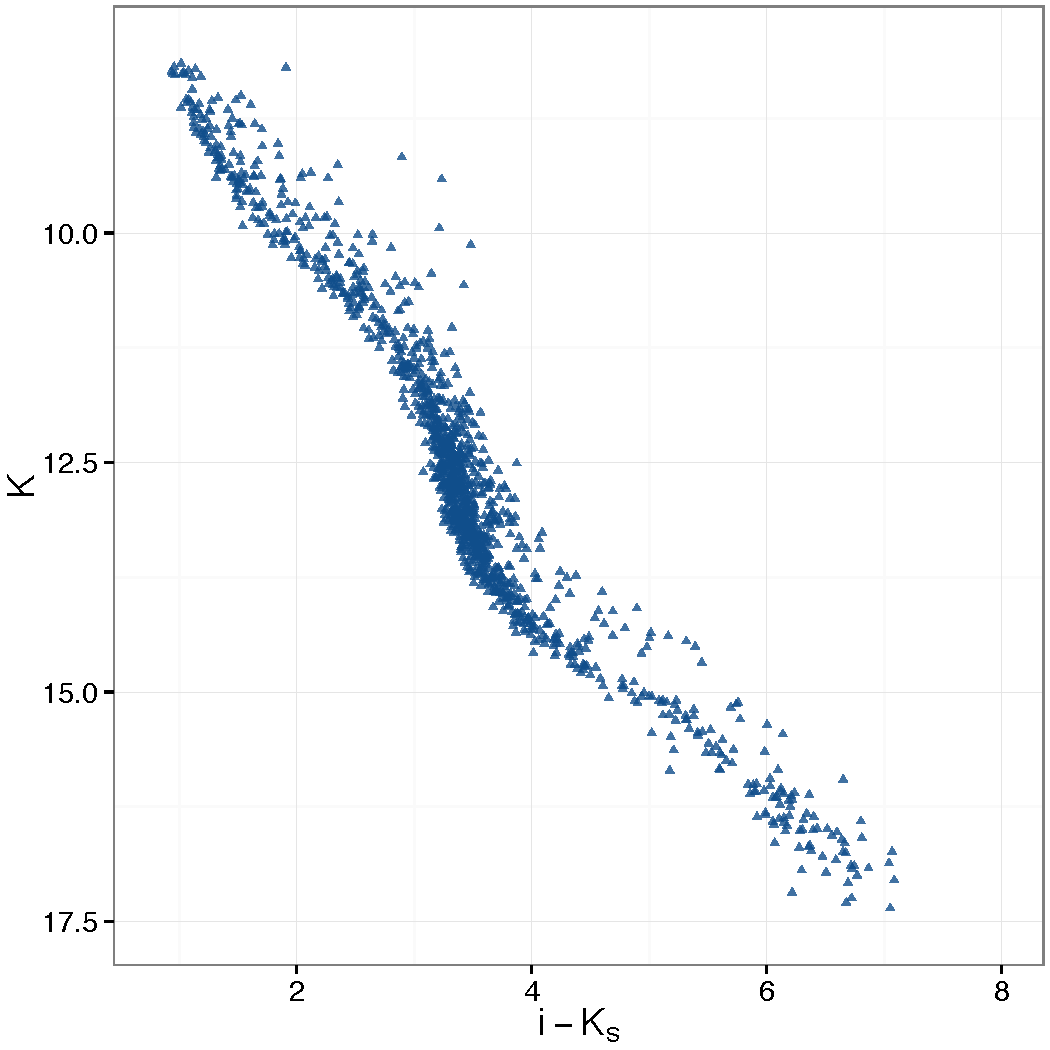
\includegraphics[page=1,height=8cm]{background/Figures/CIs.pdf}
\caption{$K_s$ vs $i-K_s$ CMD for the Pleiades candidate members of \citet{Bouy2015} with membership probability $>0.75$.}
\label{fig:CI}
\end{center}
\end{figure}

\begin{figure}[ht!]
    \centering
    \begin{subfigure}[t]{0.45\textwidth}
        \includegraphics[page=2,height=6cm]{background/Figures/CIs.pdf}
        \caption{}
        
    \end{subfigure}
    \begin{subfigure}[t]{0.45\textwidth}
      \includegraphics[page=3,height=6cm]{background/Figures/CIs.pdf}
        \caption{}
         
    \end{subfigure}
     \begin{subfigure}[t]{0.45\textwidth}
      \includegraphics[page=4,height=6cm]{background/Figures/CIs.pdf}
        \caption{}
         
    \end{subfigure}
     \begin{subfigure}[t]{0.45\textwidth}
      \includegraphics[page=5,height=6cm]{background/Figures/CIs.pdf}
        \caption{}
         
    \end{subfigure}
    \caption{CMD for the Pleiades candidate members of \citet{Bouy2015}  with membership probability $>0.75$. The magnitude $K_s$ is shown versus the colour indices: $Y-K_s$(a), $J-K_s$(b), $H-K_s$(c), and $Y-J$ (d).}
    \label{fig:otherCI}
\end{figure}

It is important to notice that if a photometric band, like $K_s$ for example, would be used to parametrise the rest of the photometric bands and the \gls{ci}. 
Then, the resulting magnitude-magnitude diagrams would provide no information to discriminate between cluster members and field objects. 


%The cluster photometric sequences, in each of the $Y,J,H,K_s$ vs \gls{ci} \glspl{cmd}, are modelled as one-to-one functions of the \emph{true} \gls{ci}. Thus,
%
%\begin{align}
%Y&=f_0(CI,\boldsymbol{\phi}),\nonumber\\
%J&=f_1(CI,\boldsymbol{\phi}),\nonumber\\
%H&=f_2(CI,\boldsymbol{\phi}),\nonumber\\
%K_s&=f_3(CI,\boldsymbol{\phi}),\nonumber
%\end{align}
%where $\boldsymbol{\phi}$ represents the set of parameters upon which the functions $f_i$ also depend on (more details below). Assuming that the magnitudes can be described by one-to-one functions of the \emph{true} colour index is an important assumption. If magnitudes were to be described by relations instead of functions, then there may be the case that one value of the colour index may result in several values of the magnitude, thus causing a non-removable discontinuity\footnote{There are three classes of discontinuities: removable, jump, and infinity ones, with increasing order of complexity for their algebraical treatment.}. This will cause degeneracies in the parametric space that will not just cripple the performance of the MCMC sampler, but also will lead to (non-removable) discontinuities in the \emph{true} colour index distribution, and therefore, in the luminosity and mass distributions. As described in Section \ref{sect:RF-2}, this the main reason for which the colour index $i-K_s$ was preferred over the other available colour indices, in spite of its large number of missing values.

After testing several functions, including the monic, Laguerre, Hermite, and Chebyshev polynomial bases, I decided to use cubic splines to model the cluster photometric sequence. Splines are piece-wise polynomial functions with more flexibility than common polynomial bases. In specific, they provide a better fit of the cluster sequence in region around \gls{ci} $\sim 3$ where other polynomial bases fail due to the high slope. 

Despite their superior flexibility when compared to the tested polynomials bases, spline series require more parameters than the latter. In addition to the coefficients of the series, they need a set of points, within their domain and in non-descending order, which are called knots. These knots represent the starting and ending points of the segments in which each piece of the pice-wise function is defined.

In addition, any spline function can be uniquely represented in terms of \glspl{bspline}. By definition, a \gls{bspline} of order $n$ is a piece-wise polynomial function of order $n-1$ in its parameter, in this case the \gls{ci}. For a given set of knots $\mathbf{t}=\{t_0,t_1,...,t_n\}$, there is one and only one \gls{bspline} representation of the spline, thus the name \glsfirst{bspline}.  In particular, any cubic spline can be represented as,

\begin{equation}
\label{eq:spline_cubic}
S_3(CI|\boldsymbol{\beta},\mathbf{t}) = \sum_i \beta_i\cdot B_{i,3}(CI|\mathbf{t}).
\end{equation}
Where $B_{i,3}$ are the cubic \glspl{bspline} given by the Cox-de Boor recursive formula, and $\boldsymbol{\beta}$ are the coefficients of the series. For more details on splines and the Cox-de Boor formula see \citet{deBoor1978}.

Despite their fitting properties, \glspl{bspline} present a problem when simultaneously inferring their coefficients and knots: there is multi-modality in the parametric space \citep{Lindstrom1999}. It means that at least more than one combination of parameters produces the same solution. To avoid this multi-modality, I decided to keep the knots fixed throughout the inference. Although this decision reduces the flexibility of the splines, it allows a still better fit than that of the tested functions (i.e. the polynomial bases). To obtain the \gls{mle} of the knots I use the algorithm of  \citet{Spiriti2013}. This algorithm, implemented in the \emph{freeknotsplines} R package, allows to simultaneously obtain the knots and the best truncation value for the spline series. It uses the \gls{bic} to select among competing models. In order to obtain both the truncation of the series and the value of the knots, I use the candidate members of \citet{Bouy2015}. The \gls{bic} indicates that seven coefficients is the best number of components for the \glspl{bspline} series, with the knots at $\mathbf{t}=\{0.8,3.22,3.22,5.17,8.0\}$. I tested different number of knots, ranging from two to nine, with five the best configuration given by the \gls{bic}. Figure \ref{fig:fitCMDs} show the spline fits to the \gls{rdr2} candidate members of \citet{Bouy2015}, resulting from the previous knots. In this fit, \glspl{emb} are excluded (see Section \ref{sect:priors} for details of how they are removed). The positions of the knots are indicated by vertical lines.

In general, the continuity of a spline function is $C^{p-k}$, with $p$ the degree of the spline, and $k$ the highest multiplicity of the knots \citep{deBoor1978}. In our case, since the knot at 3.22 has a multiplicity of two, then the resulting spline has lost one degree of continuity. It is now $C^1$ continuous. It means that the spline and its derivative are continuous, thus ensuring a smooth function. Furthermore, due to their pice-wise properties,\glspl{bspline} will enable us to model more complicated photometric sequences in which the turn-off point of the sequence may be present.

\begin{figure}[ht!]
    \centering
    \begin{subfigure}[t]{0.48\textwidth}
        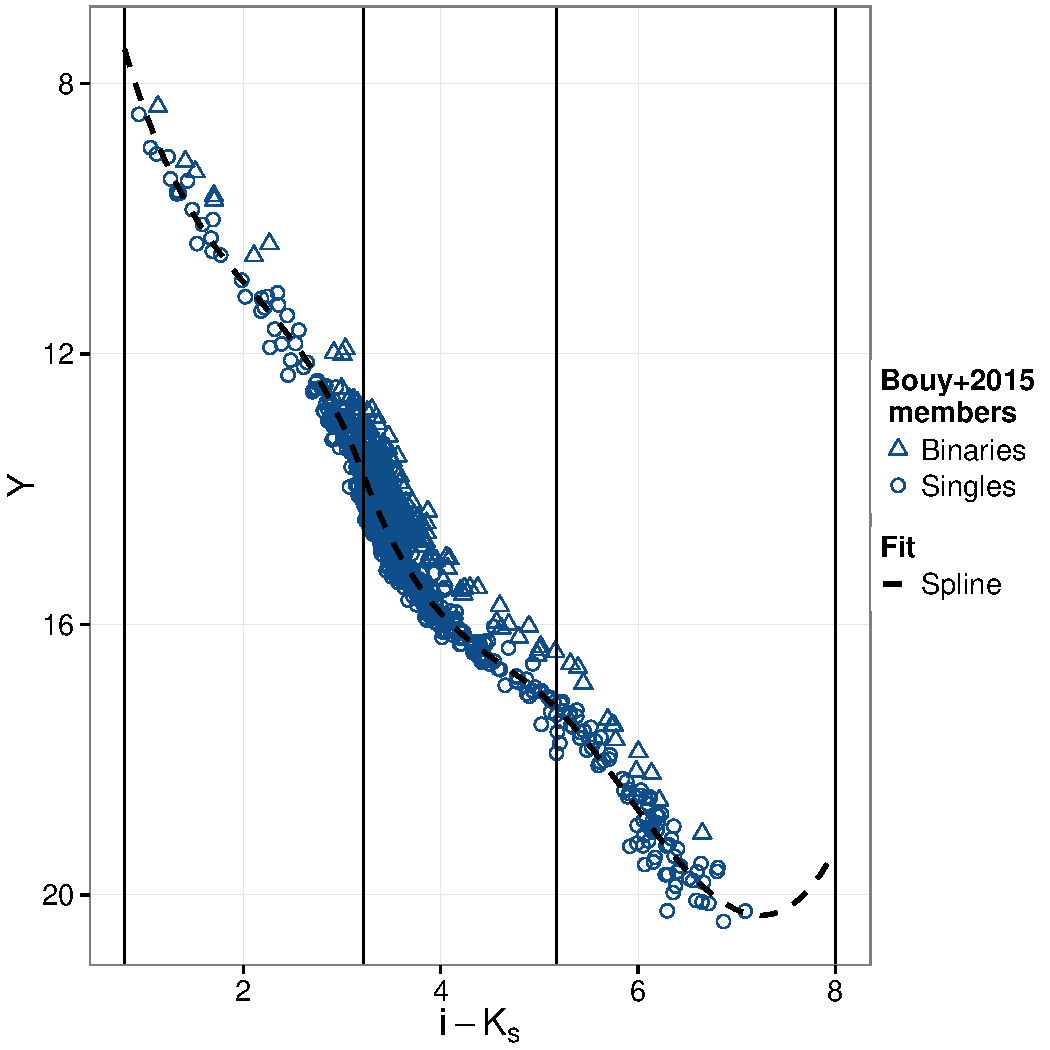
\includegraphics[page=1,height=8cm,width=\textwidth]{background/Figures/Photometry_fit.pdf}
        \caption{}
        
    \end{subfigure}
    \begin{subfigure}[t]{0.48\textwidth}
      \includegraphics[page=3,height=8cm,width=\textwidth]{background/Figures/Photometry_fit.pdf}
        \caption{}
         
    \end{subfigure}
     \begin{subfigure}[t]{0.48\textwidth}
      \includegraphics[page=5,height=8cm,width=\textwidth]{background/Figures/Photometry_fit.pdf}
        \caption{}
         
    \end{subfigure}
     \begin{subfigure}[t]{0.48\textwidth}
      \includegraphics[page=7,height=8cm,width=\textwidth]{background/Figures/Photometry_fit.pdf}
        \caption{}
         
    \end{subfigure}
\caption{Spline fits (dashed lines) to the single stars candidate members of \citet{Bouy2015} (blue circles) resulting from the use of the knots, $\mathbf{t}=\{0.8,3.22,3.22,5.17,8.0\}$, (vertical lines).}
\label{fig:fitCMDs}
\end{figure}

As I mentioned in the introduction to this Section, we assume that the observed photometric quantities are drawn from a distribution resulting from the convolution of the observed uncertainties, with the likelihood of the model prescribed by the \emph{true} quantities. We also assume that the model has an intrinsic dispersion that addresses photometric variations resulting from astrophysical phenomena not treated by our model (see Section \ref{sect:parametric_inference}). These phenomena include, but are not limited to, age, metallicity and distance dispersions, unresolved systems (other than \gls{emb}), variability, and transits. If we were to assume no \emph{true} intrinsic dispersion, then any deviation from the \emph{true} quantities would have to be explained \emph{only} on the basis of the observational uncertainties. Thus it would result in an over-simplistic model, which would underestimate the likelihood of hypothetical true cluster members. 

This photometric dispersion shows an skewed distribution \cite[see Figure 2 of][which I reproduce in Fig. \ref{fig:luminosity_dispersion}]{2008ASPC..384..200H}, which we model with a multivariate \gls{csn} distribution; see for example \citet{Gonzalez-Farias2004,Gupta2004}. Despite the fact that the \gls{csn} requires only five parameters more than a multivariate normal distribution, the computing of its density takes $\sim$ 50\% more \gls{cpu} time than that of the multivariate normal distribution. Due to computational constraints, we decided to postpone the results of the \gls{csn} until our computational resources allow it. 

Instead of using the \gls{csn}, we model the intrinsic photometric dispersion of both the cluster and \gls{emb} sequences with two multivariate normal distributions, one for the single stars sequence and other for the \gls{emb} sequence. Each of them has five dimensions corresponding to our photometric reference set: $CI,Y,J,H,K_s$. The \glspl{bspline} model the \emph{true} photometric quantities, both for the cluster sequence, $\mathbf{t}_{ph;Cs}$, and the \gls{emb}, $\mathbf{t}_{ph;Bs}$. The latter is displaced 0.75 into the bright side of the cluster sequence. In the following, the matrix $\Sigma_{clus}$, represents the covariance matrix of these two multivariate normal distribution. Since we have no reasons to believe that the intrinsic dispersion of   \gls{emb} and single stars is different, we  use only one $\Sigma_{clus}$ for both of them. By definition, covariance matrices are symmetric and positive semi-definite. Therefore, from the 25 entries in $\Sigma_{clus}$, only 15 are unique. These are also inferred from the data set.


\begin{figure}[ht!]
\begin{center}
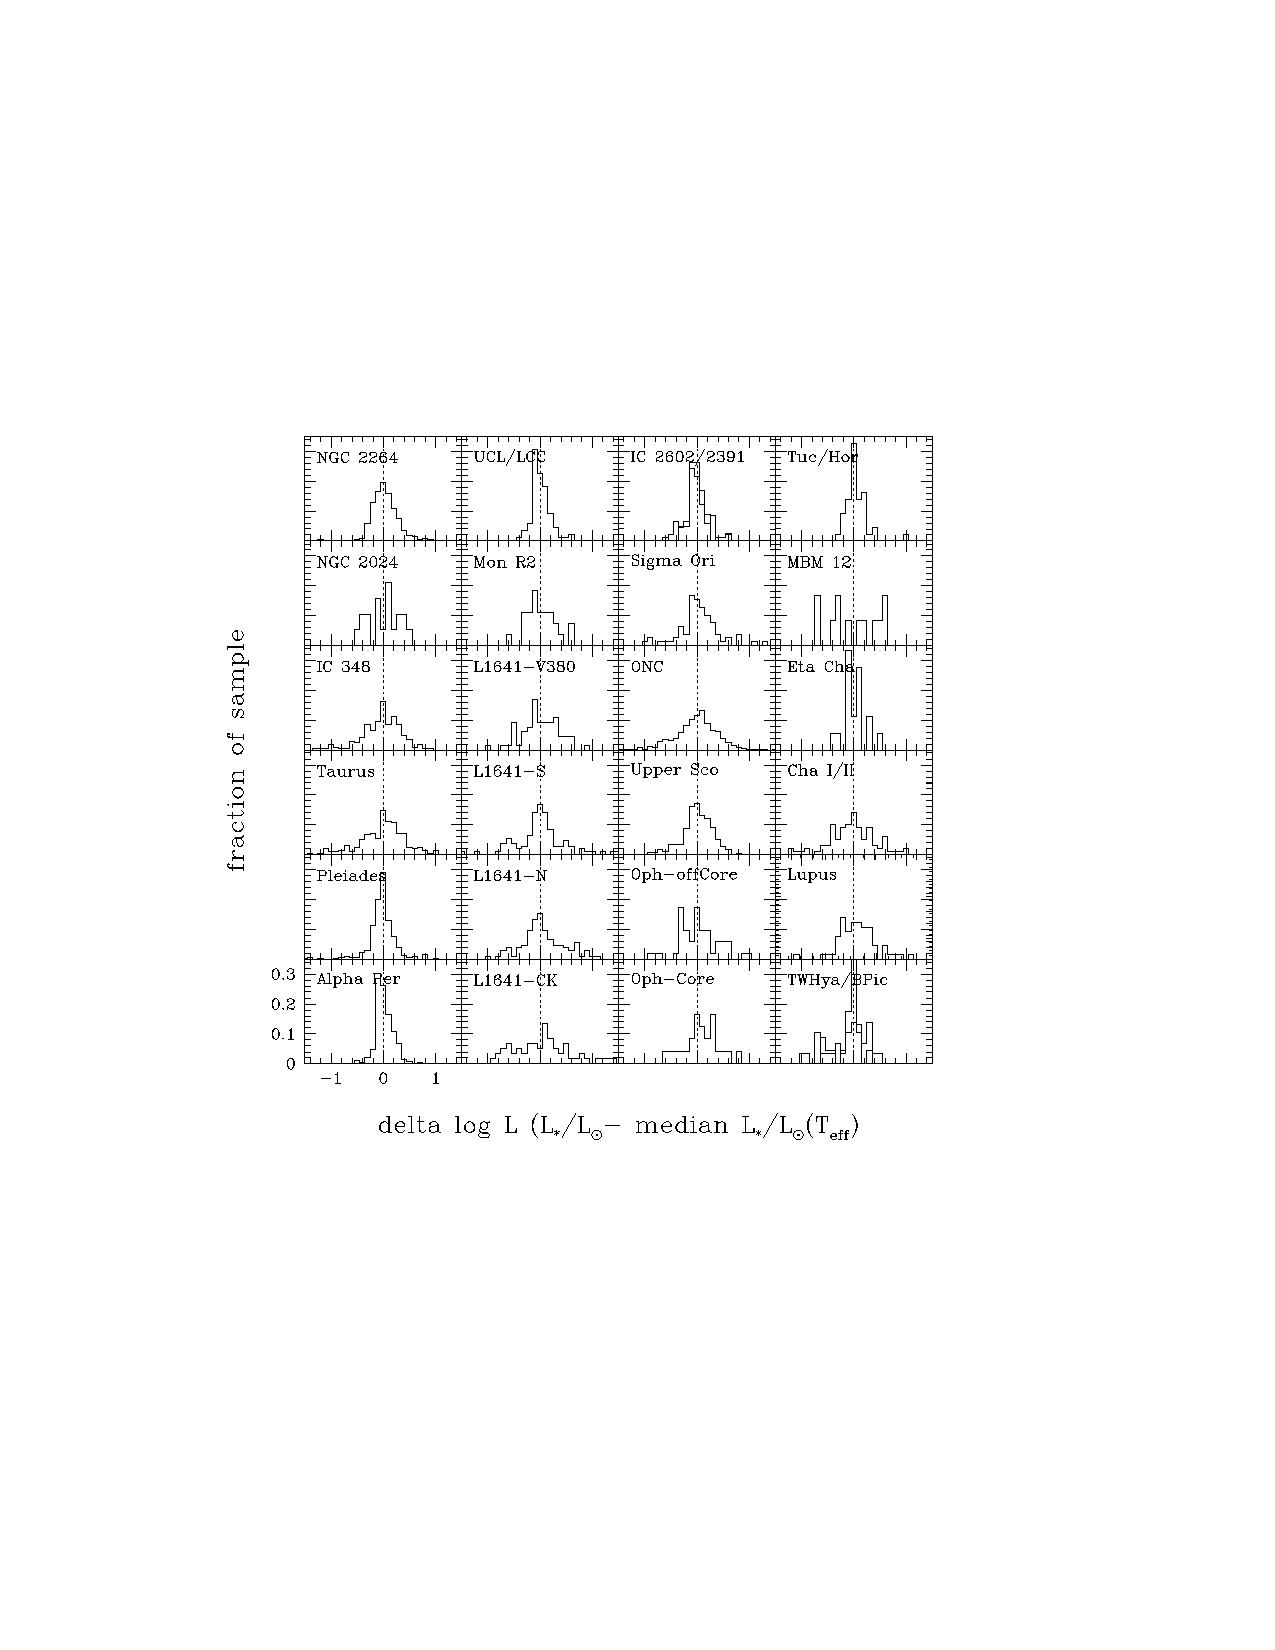
\includegraphics[width=0.8\textwidth]{background/Figures/F2_Hillenbrand2008.pdf}
\caption{Histogram of luminosity dispersion for young clusters. Reproduced from Figure 2 of \citet{2008ASPC..384..200H}, \textit{\usebibentry{2008ASPC..384..200H}{Title}}, \usebibentry{2008ASPC..384..200H}{Journal}, Vol. \usebibentry{2008ASPC..384..200H}{Volume}.}
\label{fig:luminosity_dispersion}
\end{center}
\end{figure}


Thus, the \emph{true} photometry is given by,

\begin{align}
\mathbf{t}_{ph;Cs}&= \{CI,Y,J,H,K_s\},\nonumber \\
\mathbf{t}_{ph;Bs}&=\{CI,Y-0.75,J-0.75,H-0.75,K_s-0.75\}, \nonumber
\end{align}
where
\begin{align}
\label{eq:spline_Y}
Y &=\mathcal{S}_Y(CI,\hat{\beta}_Y),\\
\label{eq:spline_J}
J &=\mathcal{S}_J(CI,\hat{\beta}_J),\\
\label{eq:spline_H}
 H &=\mathcal{S}_H(CI,\hat{\beta}_H), \\
 \label{eq:spline_K}
 K_s &=\mathcal{S}_{K_s}(CI,\hat{\beta}_{K_s}), 
\end{align}
with $\hat{\beta}_{i}, i\in\{Y,J,H,K_s\}$ the vectors of seven coefficients of the \glspl{bspline} for the $Y,J,H,K_s$ bands.  For the sake of simplicity I denote this $4\times7$ coefficients matrix as $\boldsymbol{\beta}$.

Since the photometry of the \gls{emb} is a linear transformation, $T_{Bs}$, of the mean \emph{true} photometry of cluster sequence, no extra parameters are required. Therefore, 

\begin{align}
\mathbf{t}_{ph;Cs} &= \boldsymbol{\mathcal{S}}(CI, \boldsymbol{\beta}) \label{eq:trueph_Cs}\\
\mathbf{t}_{ph;Bs} &=T_{Bs}( \boldsymbol{\mathcal{S}}(CI, \boldsymbol{\beta})).
\label{eq:trueph_Bs}
\end{align}

Thus, cluster and \gls{emb} likelihoods of an object with photometric measurements $\mathbf{d}_{ph}$, and standard uncertainties $\mathbf{u}_{ph}$, are:
\begin{align}
\label{eq:lik-seq}
 p_{Cs}(\mathbf{d}_{ph}| CI, \boldsymbol{\beta},\Sigma_{clus},\mathbf{u}_{ph})={\mathcal{N}}(\mathbf{d}_{ph}|\mathbf{t}_{ph;Cs}, \mathbf{u}_{ph}+\Sigma_{clus}),\nonumber \\
p_{Bs}(\mathbf{d}_{ph}| CI, \boldsymbol{\beta},\Sigma_{clus}, \mathbf{u}_{ph})={\mathcal{N}}(\mathbf{d}_{ph}|\mathbf{t}_{ph;Bs}, \mathbf{u}_{ph}+\Sigma_{clus}),
\end{align}
where $\mathbf{t}_{ph;Cs}$ and $\mathbf{t}_{ph;Bs}$ are given by Equations \ref{eq:trueph_Cs} and \ref{eq:trueph_Bs}, respectively.

Since the splines are parametrised by the true \gls{ci} of each object, we have more parameters than objects in our data set \footnote{Although this sounds crazy, the rules of probability calculus do not discard this possibility.}. This \emph{true} \gls{ci} is unknown even if its observed value is not missing. We solve this problem (it is a computational problem!) by marginalising these nuisance parameters. 

To marginalise these \glspl{ci} we need a prior, which we provide in a hierarchical way (thus the name Bayesian Hierarchical model). This marginalisation leaves behind a precise estimate of the parameters of the prior distribution. Paradoxically, all objects, even those without a measurement of the \gls{ci}, contribute to this estimate. Here lays the force of the \gls{bhm} .

We model the prior of the \emph{true} \gls{ci} as a truncated ($0.8\leq CI \leq8$) univariate \gls{gmm} with five components, whose parameters are also inferred from the data. We choose five components as suggested by the \gls{bic} computed from the \gls{em} algorithm for \gls{gmm} applied to the \gls{rdr2} candidate members of \citet{Bouy2015} \textbf{with observed \glspl{ci}}. I tested larger number of components in the mixture (up to ten), but the posterior distribution did not changed significantly, thus indicating that the \gls{bic} value was a proper assumption. \textbf{Figure \ref{fig:fitCI} shows the fit of this five component univariate \gls{gmm} to the \gls{rdr2} candidate members of \citet{Bouy2015} with observed \glspl{ci}. Notice that these fits are only performed to obtain the best number of components in the \gls{gmm}.}

\begin{figure}[ht!]
\begin{center}
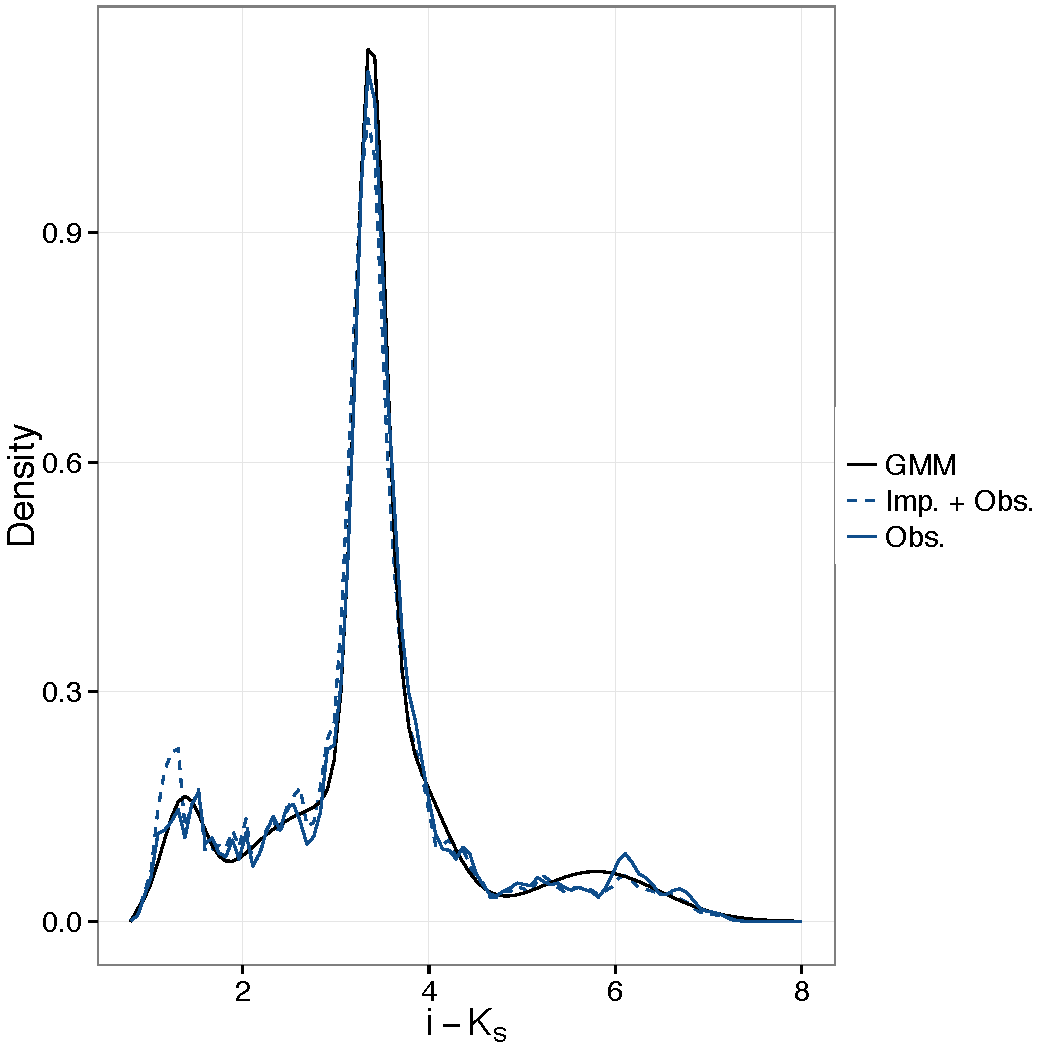
\includegraphics[page=1,width=\textwidth]{background/Figures/BIC_Color_fit.pdf}
\caption{Distribution of observed \glspl{ci} of the candidate members of \citet{Bouy2015} (solid blue line). The uncertainties are taken into account by performing a \gls{kde} in which each object kernel is Gaussian with bandwidth equal to its observed uncertainty. Also shown is the five components \gls{gmm} fitted to this data (solid black line). For the sake of completeness, I also show the distribution of imputed and observed $\glspl{ci}$ for all candidate members of \citet{Bouy2015} (dashed blue line). Missing \glspl{ci} where imputed with those of the closet euclidean neighbour in the five dimensional space.}
\label{fig:fitCI}
\end{center}
\end{figure}



The \gls{gmm} modelling the prior of the \emph{true} \gls{ci} is 

\begin{equation}
\label{eq:colordist}
p(CI|\boldsymbol{\pi}_{CI},\boldsymbol{\mu}_{CI},\boldsymbol{\sigma}_{CI})= \sum_{i=1}^5 \pi_{CI,i} \cdot \mathcal{N}_t(CI| \mu_{CI,i},\sigma_{CI,i}).
\end{equation}

In this last Equation, the symbol $\mathcal{N}_t$ stands for the truncated ($0.8<CI<8$) univariate normal distribution.

Then, the marginalisation of \gls{ci} runs as follows:
\begin{align}
\label{eq:clmarginalps}
 p_{Cs}(\mathbf{d}_{ph}| \boldsymbol{\theta}_c,\mathbf{u}_{ph})&=\int p_{Cs}(\mathbf{d}_{ph},CI| \boldsymbol{\theta}_c,\mathbf{u}_{ph}) \cdot \mathrm{d}CI \nonumber \\
 &=\int p_{Cs}(\mathbf{d}_{ph}|CI, \boldsymbol{\theta}_c,\mathbf{u}_{ph}) \cdot p_{Cs}(CI| \boldsymbol{\theta}_c,\mathbf{u}_{ph})\cdot \mathrm{d}CI 
\end{align}
\begin{align}
\label{eq:clmarginalpb}
p_{Bs}(\mathbf{d}_{ph}| \boldsymbol{\theta}_c,\mathbf{u}_{ph})&=\int p_{Bs}(\mathbf{d}_{ph},CI| \boldsymbol{\theta}_c,\mathbf{u}_{ph})\cdot \mathrm{d}CI \nonumber \\
 &=\int p_{Bs}(\mathbf{d}_{ph}|CI, \boldsymbol{\theta}_c,\mathbf{u}_{ph})\cdot p_{Bs}(CI| \boldsymbol{\theta}_c,\mathbf{u}_{ph})\cdot \mathrm{d}CI.
\end{align}
In these Equations, $\boldsymbol{\theta}_c$ stands for all cluster parameters related to photometry, and the first and second terms of the integrals in the last equalities correspond to Equations \ref{eq:lik-seq} and \ref{eq:colordist}, respectively. The distribution of \gls{ci} depends only on $\boldsymbol{\pi}_{CI},\boldsymbol{\mu}_{CI},\boldsymbol{\sigma}_{CI}$, thus, the cluster and equal-mass binaries likelihoods of datum $\mathbf{d}_{ph}$ are 
\begin{align}
\label{eq:lik-seq2}
 &p_{Cs}(\mathbf{d}_{ph}|\boldsymbol{\pi}_{CI},\boldsymbol{\mu}_{CI},\boldsymbol{\sigma}_{CI},\boldsymbol{\beta},\Sigma_{clus},\mathbf{u}_{ph}) \nonumber \\
 &=\int{\mathcal{N}}(\mathbf{d}_{ph}|\boldsymbol{\mathcal{S}}(CI, \boldsymbol{\beta}), \mathbf{u}_{ph}+\Sigma_{clus})\cdot \sum_{i=1}^5 \pi_{CI,i}\cdot \mathcal{N}_t(CI| \mu_{CI,i},\sigma_{CI,i}) \cdot \mathrm{d}CI\nonumber \\
&p_{Bs}(\mathbf{d}_{ph}|\boldsymbol{\pi}_{CI},\boldsymbol{\mu}_{CI},\boldsymbol{\sigma}_{CI}, \boldsymbol{\beta},\Sigma_{clus}, \mathbf{u}_{ph})\nonumber \\
&=\int{\mathcal{N}}(\mathbf{d}_{ph}|T_{Bs}( \boldsymbol{\mathcal{S}}(CI, \boldsymbol{\beta})), \mathbf{u}_{ph}+\Sigma_{clus}) \cdot \sum_{i=1}^5 \pi_{CI,i}\cdot \mathcal{N}_t(CI| \mu_{CI,i},\sigma_{CI,i}) \cdot \mathrm{d}CI.
\end{align}

The observed \gls{ci} and magnitudes help us  to reduce the computing time of the marginalisation integral. We use them to discard  regions of the integral in which the argument is almost zero (i.e. far from the measured values). Although we allow the nuisance parameters \glspl{ci} to have all their possible values, the data, by means of the likelihood, give us information about the distribution of these individual nuisance parameters. To use this information, we proceed as follows. First, we compare the observed photometry to the true one (i.e. the cluster sequence given by the splines). For it we use a grid of 300 points uniformly distributed in the domain of \gls{ci} ($0.8<CI<8$)\footnote{\label{foot:extendedCI}As explained in Section \ref{sect:RDR2}, if this \gls{ci} range will have covered that of all the objects in the \gls{ddr2} data set, the marginalisation integral would have to be computed over the extended \gls{ci} range. Therefore, the computing time of the \gls{bhm}  would have also increased proportionally to the number of extra points in this integral.}. Then, we find the point, $p$, of the grid that is closest to the vector of the observed photometry.  Distance is computed under  the Mahalanobis metric. This metric takes into account the observational uncertainty, $\mathbf{u}_{ph}$, and the intrinsic dispersion of the cluster sequence, $\Sigma_{clus}$. Finally, the limits of the marginalisation integral  are defined as those given by a ball of 3.5 Mahalanobis distances around point $p$. Contributions outside this ball are negligible to the integral ($< 4\times10^{-4}$).

\subsubsection{Proper motion model of EMB and single stars}
\label{sect:cluster_pm}
As mentioned before, we assume that the cluster population has two subpopulations: single and \gls{emb} stars.
We model the proper motions of these two subpopulations with independent \gls{gmm}. If the cluster is virialised (see Chapter \ref{chap:pleiades}), we can assume that{ the distribution of its velocity modulus} is almost Maxwellian (Maxwell-Boltzman distribution). Therefore a \gls{gmm} is a reasonable {approximation}. Furthermore, in the absence of external forces, a virialised system is expected to have spherical symmetry both in its spatial and velocity distributions. Thus we can safely assume that the gaussians within each \gls{gmm} are concentric, thus they share the same mean. However we allow independent means for both single and \gls{emb} subpopulations. The assumption of spherical symmetry may be a weak one in the presence of the galactic potential. It can perturb the cluster and deviate its spatial and velocity distribution from spherical symmetry. Furthermore, the ellipticity of the spatial distribution, which has been reported to be no-negligible \cite[$\epsilon=0.17$, according to ][]{Raboud1998}, can be due to projection effects that further deviate the observed velocity distribution profile from spherical symmetry. Nevertheless, since we model the covariance matrices of the \gls{gmm} of both single and \gls{emb}, as full covariance matrices, any departure from the spherical symmetry in the velocity distribution can still be modelled by the non-diagonal entries of these matrices.


We infer the parameters of these \glspl{gmm} as part of our Bayesian hierarchical model. However we set a priori the number of gaussians in each \gls{gmm}. Not doing so will demand a technique in which the model parameters can be augmented. Although such techniques already exist, they are still under computational development \cite[see][for a review of reversible jump \gls{mcmc}]{Fan2011}.

Using the \gls{em} algorithm for \gls{gmm} and the proper motions of the \gls{rdr2} candidate members of \citet{Bouy2015}, I obtained the \glspl{mle} for the \gls{gmm} likelihoods. I did this for configurations of \gls{gmm} ranging from one to six components. The \gls{bic} (Eq. \ref{eq:BIC}) suggested four and two components for the cluster and \gls{emb} \glspl{gmm}, respectively. \textbf{Figures \ref{fig:fitPM} and \ref{fig:fitPMprojections} show the Gaussians fitted, and the marginal densities. Notice that this fit is only illustrative of the number of components used for these \glspl{gmm}. } Since covariance matrices are always symmetric, only three parameters are needed to fully specify the covariance matrices of these bivariate normal distributions.

\begin{figure}[ht!]
    \centering
       \begin{subfigure}[t]{0.48\textwidth}
      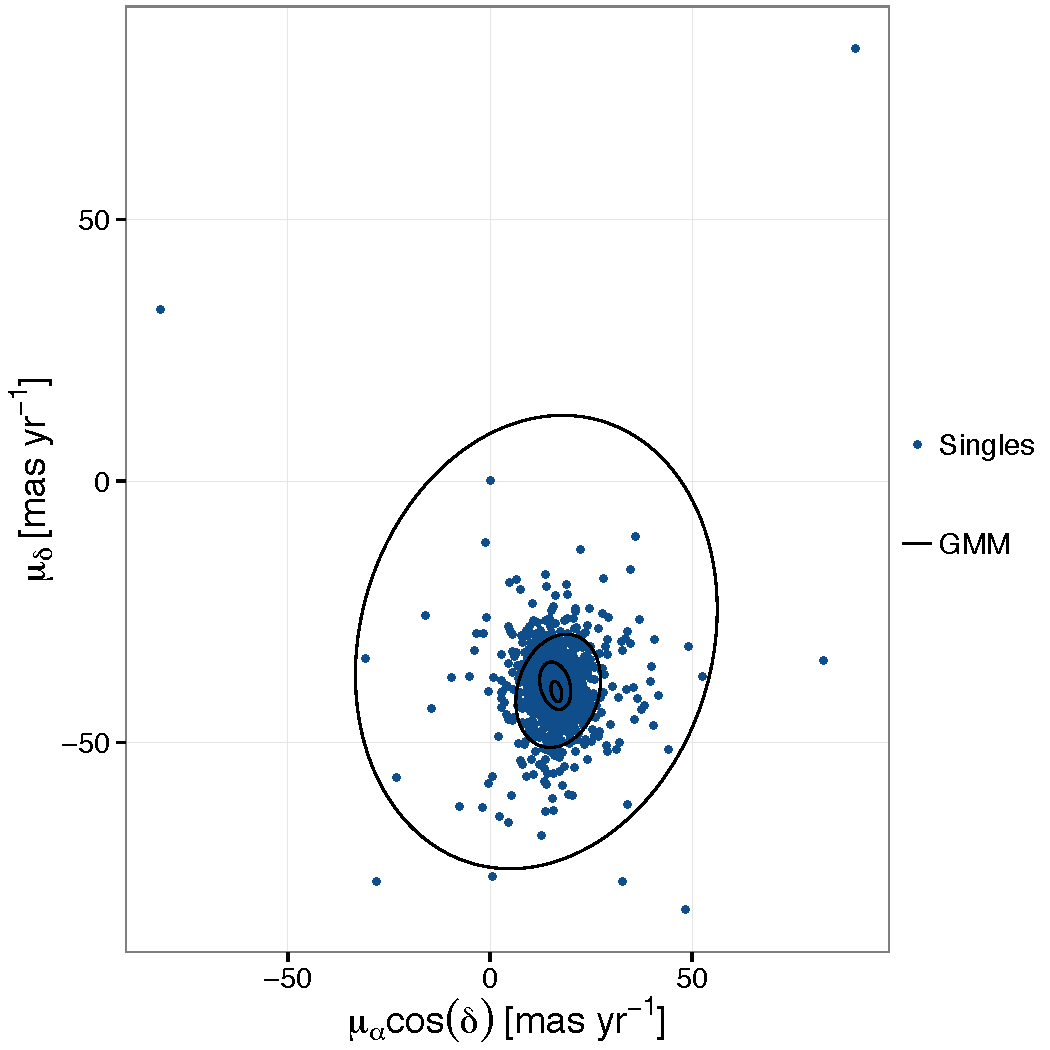
\includegraphics[page=1,height=8cm,width=\textwidth]{background/Figures/BIC_PM_Cs_fit.pdf}
        \caption{}
    \end{subfigure}
     \begin{subfigure}[t]{0.48\textwidth}
      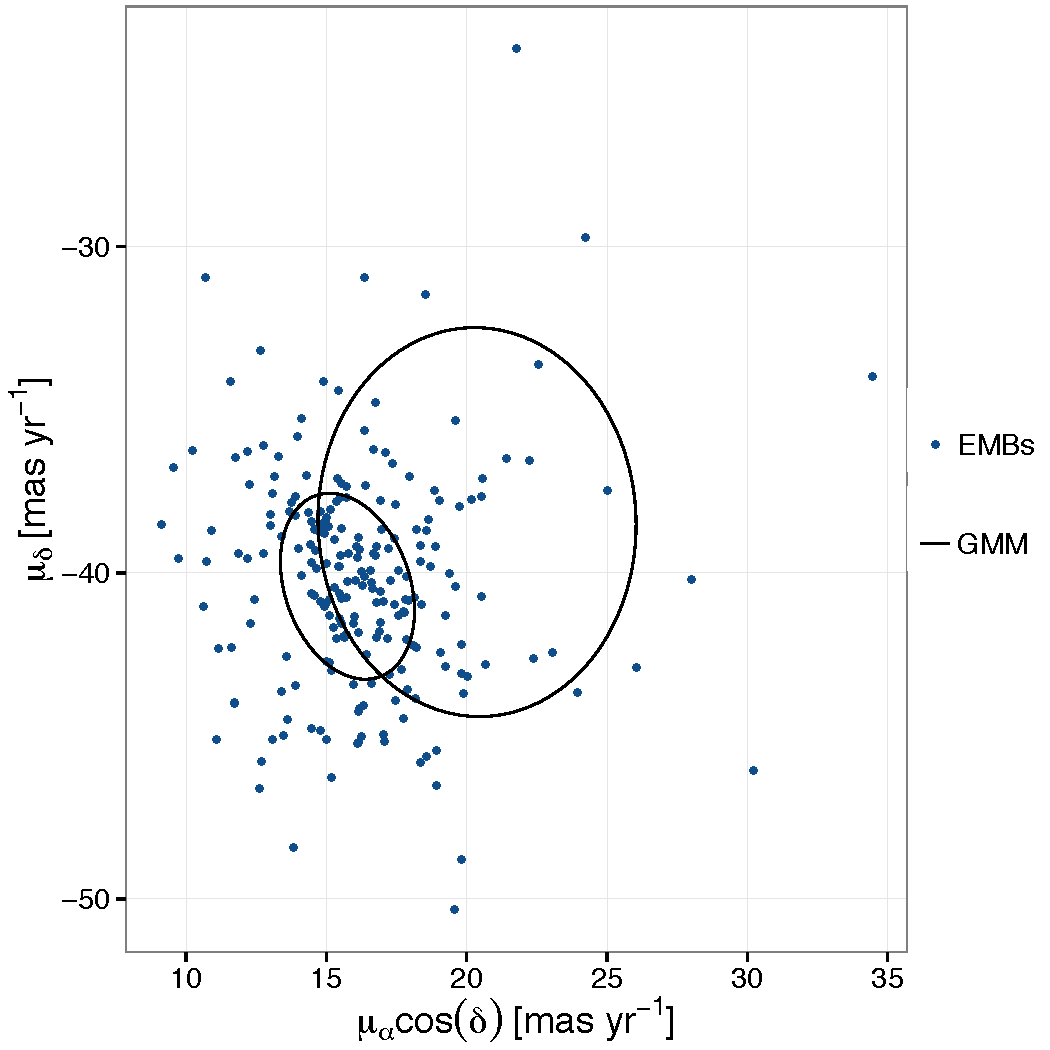
\includegraphics[page=1,height=8cm,width=\textwidth]{background/Figures/BIC_PM_Bs_fit.pdf}
        \caption{}
    \end{subfigure}
\caption{Single stars (a) and \glspl{emb} (b) members of \citet{Bouy2015} (blue circles) in the \gls{rdr2}. Also shown the fitted \glspl{gmm} with four and two components according to the \gls{bic}.}
\label{fig:fitPM}
\end{figure}


\begin{figure}[ht!]
    \centering
    \begin{subfigure}[t]{0.48\textwidth}
        \includegraphics[page=2,height=8cm,width=\textwidth]{background/Figures/BIC_PM_Cs_fit.pdf}
        \caption{}
    \end{subfigure}
    \begin{subfigure}[t]{0.48\textwidth}
      \includegraphics[page=3,height=8cm,width=\textwidth]{background/Figures/BIC_PM_Cs_fit.pdf}
        \caption{}
    \end{subfigure}
     \begin{subfigure}[t]{0.48\textwidth}
      \includegraphics[page=2,height=8cm,width=\textwidth]{background/Figures/BIC_PM_Bs_fit.pdf}
        \caption{}
    \end{subfigure}
     \begin{subfigure}[t]{0.48\textwidth}
      \includegraphics[page=3,height=8cm,width=\textwidth]{background/Figures/BIC_PM_Bs_fit.pdf}
        \caption{}
    \end{subfigure}
\caption{Marginal distributions of the single stars (a and b) and \glspl{emb} (c and d) candidate members of \citet{Bouy2015} in the \gls{rdr2} (blue lines). The densities result of a \gls{kde} with gaussian kernel and bandwidth equal to the individual uncertainties. Also shown the marginal distribution resulting from the fitted \glspl{gmm} of Fig. \ref{fig:fitPM} (black lines).}
\label{fig:fitPMprojections}
\end{figure}



The cluster (subindex $Cs$) and \gls{emb} (subindex $Bs$) likelihoods of an object with proper motions measurements $\mathbf{d}_{pm}$, and uncertainties $\mathbf{u}_{pm}$, are

\begin{align}\label{eq:lik-pm-cs}
p_{Cs}(\mathbf{d}_{pm}| \boldsymbol{\pi}_{Cs}, \boldsymbol{\mu}_{Cs},\boldsymbol{\Sigma}_{Cs},\mathbf{u}_{pm})
&= \sum_{i=1}^4\pi_{Cs,i}\cdot \mathcal{N}(\mathbf{d}_{pm} | \boldsymbol{\mu}_{Cs},\Sigma_{Cs,i}+\mathbf{u}_{pm})
\end{align}
\begin{align}
p_{Bs}(\mathbf{d}_{pm}| \boldsymbol{\pi}_{Bs}, \boldsymbol{\mu}_{Bs},\boldsymbol{\Sigma}_{Bs},\mathbf{u}_{pm})
&= \sum_{i=1}^2\pi_{Bs,i}\cdot \mathcal{N}(\mathbf{d}_{pm} | \boldsymbol{\mu}_{Bs},\Sigma_{Bs,i}+\mathbf{u}_{pm}).
\label{eq:lik-pm-bs}
\end{align}

Finally, combining the proper motions and photometric models, the total cluster likelihood of an object with measurement $\mathbf{d}$, and uncertainties $\mathbf{u}$, is

\begin{align}
p_c(\mathbf{d}|\boldsymbol{\theta}_c,\mathbf{u})=\pi_{CB}&\cdot p_{Cs}(\mathbf{d}_{pm}| \boldsymbol{\pi}_{Cs}, \boldsymbol{\mu}_{Cs},\boldsymbol{\Sigma}_{Cs},\mathbf{u}_{pm}) \cdot  p_{Cs}(\mathbf{d}_{ph}|\boldsymbol{\pi}_{CI},\boldsymbol{\mu}_{CI},\boldsymbol{\sigma}_{CI},\boldsymbol{\beta},\Sigma_{clus},\mathbf{u}_{ph})\nonumber\\
+(1-\pi_{CB})&\cdot p_{Bs}(\mathbf{d}_{pm}| \boldsymbol{\pi}_{Bs}, \boldsymbol{\mu}_{Bs},\boldsymbol{\Sigma}_{Bs},\mathbf{u}_{pm}) \cdot  p_{Bs}(\mathbf{d}_{ph}|\boldsymbol{\pi}_{CI},\boldsymbol{\mu}_{CI},\boldsymbol{\sigma}_{CI}, \boldsymbol{\beta},\Sigma_{clus}, \mathbf{u}_{ph}),
\end{align}

where $\pi_{CB}$ is the parameter representing the proportion or fraction of single cluster sequence stars in the single-\gls{emb} mixture model. The photometric and proper motions likelihoods are given by Equations \ref{eq:lik-seq2}, and \ref{eq:lik-pm-cs} and \ref{eq:lik-pm-bs}, respectively.

\textbf{Before ending this Section, in Table \ref{tab:cluster_parameters}, I list the groups (proper motions of photometry), symbols, dimensions and meanings of the cluster parameters. Furthermore, Table \ref{tab:all_parameters} lists all parameters in the \gls{bhm} (field and cluster) together with their symbols, status (i.e. if they are free or fixed, and the sample from which their values were derived, in case they are fixed), a brief description of their meaning, and the Section and Equation in which they are explained. Finally, Fig. \ref{fig:PGMBHM} gives the graphical representation of the \gls{bhm} in the form of a \gls{pgm}.}

\input{background/Tables/ClusterParameters.txt}

\input{background/Tables/AllParameters.txt}



\begin{figure}[ht!]
  \begin{center}
  \resizebox{0.8\textwidth}{!}{
%\documentclass[12pt]{amsart}
%\usepackage{bm}
%\usepackage{color}
%\usepackage[usenames,dvipsnames,svgnames,table]{xcolor}
%\usepackage{tikz}
%\usetikzlibrary{arrows,arrows.meta,shapes,decorations.pathmorphing,positioning,intersections,calc,backgrounds}
\tikzstyle{line} = [draw, -latex']
\tikzstyle{marginalized}=[black, {Circle[color=black,length=3pt]-latex[]}]
%\tikzstyle{con} = [thick, dashed, draw, angle 90 reversed-angle 90 reversed]
%\tikzset{
%    box1/.style={%
%        draw=black, thick,
%        rectangle,
%        rounded corners,
%        minimum height=4cm,
%        minimum width=4cm
%    },
%    snake arrow/.style=
%{->,
%decorate,
%decoration={snake,amplitude=.4mm,segment length=2mm,post length=1mm}}
%}
%
%
%% See the ``Article customise'' template for come common customisations
%
%%%% BEGIN DOCUMENT
%\begin{document}
%\begin{figure}[tb]
%  \begin{center}
%  \resizebox{0.9\linewidth}{!}{
\begin{tikzpicture}[>=stealth', node distance = 1cm, every node/.style={rectangle,fill=white}]

%############### Principal block ###################
% Variables 
\node[draw, fill = gray!20, circle, label={[name=x_i_lab,xshift=-10pt,yshift=3pt]below:$\boldsymbol{d}$}] (x_i) at (0,0) {$[7]$};
\node[draw, circle, label={[name=pi_lab,xshift=-10pt,yshift=3pt]below:$\pi$}] (pi) [above = of x_i] {$[1]$};
\node[draw, fill = gray!20, label={[name= alpha_lab]above:$\boldsymbol{\alpha}$}] (alpha) [above = of pi] {$[2]$};

% relations
\path[line] (alpha) -> (pi);
\draw[marginalized] (pi) -- (x_i);
% plates
\begin{pgfonlayer}{background}
\node (rect) at (x_i) [xshift = 0pt, yshift = -3pt, draw, rounded corners, thick, minimum width=50pt, 
minimum height=50pt, line width=1pt, fill=yellow!90!blue, fill opacity=0.3] (rect1) {};
\end{pgfonlayer}
\node[anchor=south east,inner sep=5pt, fill = none] at (rect1.south east) {$N$};

%############# NON-MEMBERS ##############################
\node[draw, fill = gray!20, label={[name = mu_nm_pm_lab,xshift=0pt,yshift=2pt]above:$\boldsymbol{\mu}_{f,pm}$}] (mu_nm_pm) [left = of x_i,xshift=-120pt,yshift=100pt] {$[2]$};

\node[draw, fill = gray!20, label={[name = sg_nm_pm_lab,xshift=0pt,yshift=2pt]above:$\Sigma_{f,pm}$}] (sg_nm_pm) [right = of mu_nm_pm,yshift=0pt] {$[2,2]$};
\node[draw, fill = gray!20, label={[name = pi_nm_pm_lab,xshift=0pt,yshift=0pt]above:$\pi_{f,pm}$}] (pi_nm_pm) [right = of sg_nm_pm,xshift=5pt,yshift=0pt] {[8]};

\node[draw, fill = gray!20, label={[name = mu_nm_phot_lab,xshift=0pt,yshift=2pt]below:$\boldsymbol{\mu}_{f,ph}$}] (mu_nm_phot) [left = of x_i,xshift=-120pt,yshift=-60pt] {$[5]$};

\node[draw, fill = gray!20, label={[name = sg_nm_phot_lab,xshift=0pt,yshift=2pt]below:$\Sigma_{f,ph}$}] (sg_nm_phot) [right = of mu_nm_phot,yshift=0pt] {$[5,5]$};
\node[draw, fill = gray!20, label={[name = pi_nm_phot_lab,xshift=0pt,yshift=0pt]below:$\pi_{f,ph}$}] (pi_nm_phot) [right = of sg_nm_phot,xshift=5pt,yshift=0pt] {[14]};


\begin{pgfonlayer}{background}
\node (rect) at (mu_nm_pm) [xshift = 35pt, yshift = 5pt, draw, rounded corners, thick, minimum width=110pt, 
minimum height=50pt, line width=1pt, fill=gray!20, fill opacity=0.5] (rect2) {};
\end{pgfonlayer}
\node[anchor=south east,inner sep=5pt, fill = none] at (rect2.south east) {7};

\begin{pgfonlayer}{background}
\node (rect) at (mu_nm_phot) [xshift = 35pt, yshift = -4pt, draw, rounded corners, thick, minimum width=110pt, 
minimum height=50pt, line width=1pt, fill=gray!20, fill opacity=0.5] (rect2) {};
\end{pgfonlayer}
\node[anchor=south east,inner sep=5pt, fill = none] at (rect2.south east) {14};

\draw [->,name path=curve] (mu_nm_pm) to [out = -90, in = 180, looseness=1] (x_i);
\draw [->,name path=curve] (sg_nm_pm) to [out = -90, in = 180, looseness=1] (x_i);
\draw [->,name path=curve] (pi_nm_pm) to [out = -90, in = 180, looseness=1] (x_i);

\draw [->,name path=curve] (mu_nm_phot) to [out = 90, in = 180, looseness=1] (x_i);
\draw [->,name path=curve] (sg_nm_phot) to [out = 90, in = 180, looseness=1] (x_i);
\draw [->,name path=curve] (pi_nm_phot) to [out = 90, in = 180, looseness=1] (x_i);
%############# MEMBERS ##############################
% photometry block
\node[draw, circle, label={[name = t_phot_lab,xshift=-10pt,yshift=3pt]below:$$}] (t_phot) [right = of x_i,xshift=100pt,yshift=25] {$\boldsymbol{t}_{ph}$};
\node[draw, circle, label={[name = idx_clr_lab,xshift=-10pt,yshift=3pt]below:$$}] (idx_clr)  [above = of t_phot]  {$CI$};
\node[draw, circle, label={[name = sg_phot_lab,xshift=-10pt,yshift=3pt]below:$\Sigma_{clus}$}] (sg_phot) [left = of idx_clr,xshift=10pt] {$[15]$};
\node[draw, circle, label={[name = pi_phot_lab,xshift=-15pt,yshift=3pt]below:$\pi_{CB}$}] (pi_phot) [below= of x_i, xshift=0pt,yshift=-0pt] {$[1]$};
\node[draw, circle, label={[name = beta_lab,xshift=-10pt,yshift=3pt]below:$\boldsymbol{\beta}$}] (beta) [right = of idx_clr] {$[4,7]$};
\node[draw, circle, label={[name = mu_clr_lab,xshift=-10pt,yshift=3pt]below:$\mu_{CI}$}] (mu_clr) [above = of idx_clr] {$[1]$};
\node[draw, circle, label={[name = pi_clr_lab,xshift=-10pt,yshift=3pt]below:$\pi_{CI}$}] (pi_clr)  [left = of mu_clr]  {$[4]$};
\node[draw, circle, label={[name = sigma_clr_lab,xshift=-5pt,yshift=3pt]below:$\sigma_{CI}$}] (sigma_clr) [right = of mu_clr ]{$[1]$};

\draw (idx_clr)  node[fill=none,minimum size=16pt,draw] {};

\node[draw, fill = gray!20, label={[name = mu_beta_lab]above:$\boldsymbol{\mu}_{\beta}$}] (mu_beta) [right = of beta]{$[4,7]$};
\node[draw, fill = gray!20, label={[name = sg_beta_lab]above:$\boldsymbol{\sigma}_{\beta}$}] (sg_beta) [above = of mu_beta] {$[7]$};
\node[draw, fill = gray!20, label=below:$\boldsymbol{\alpha}_{CB}$] (alpha_phot) [below=of pi_phot] {$[2]$};
\node[draw, fill = gray!20, label={[name = alpha_clr_0_lab]above:$\boldsymbol{\alpha}_{CI}$}] (alpha_clr_0) [above = of pi_clr] {$[5]$};
\node[draw, fill = gray!20, label={[name = rg_clr_lab]above:$rg_{CI}$}] (rg_clr) [above = of mu_clr,xshift=0pt] {$[2]$};
\node[draw, fill = gray!20, label={[name = eta_clr_lab]above:$\eta$}] (eta_clr) [above = of sigma_clr,xshift=0pt] {$[1]$};
\node[draw, fill = gray!20, label={[name = nu_phot_lab]above:$\nu$}] (nu_phot) [left = of sg_phot,yshift=0pt] {$[1]$};
\node[draw, fill = gray!20, label={[name = A_phot_lab]above:$\boldsymbol{A}_{ph}$}] (A_phot) [above = of nu_phot,yshift=0pt] {$[5]$};
\begin{pgfonlayer}{background}
\node (rect) at (idx_clr) [xshift = 0pt, yshift = 25pt, draw, rounded corners, thick, minimum width=170pt,
 minimum height=120pt, line width=1pt, fill=black!20!red, fill opacity=0.5] (rect4) {};
\end{pgfonlayer}

\begin{pgfonlayer}{background}
\node (rect) at (mu_clr) [xshift = 30pt, yshift = -5pt, draw, rounded corners, thick, minimum width=100pt,
 minimum height=60pt, line width=1pt, fill=none] (rect5) {};
\end{pgfonlayer}
\node[anchor=south east,inner sep=5pt, fill=none] at (rect5.south east) {$5$};


\path [line,dashed] (idx_clr) -> (t_phot);
\path [line,dashed] (beta) -> (t_phot);
\path[line] (mu_clr) -> (idx_clr);
\path[line] (sigma_clr) -> (idx_clr);
\draw[marginalized] (pi_clr) to (idx_clr);
\path[line] (mu_beta) -> (beta);
\path[line] (sg_beta) -> (beta);
\path[line] (alpha_clr_0) -> (pi_clr);
\path[line] (rg_clr) -> (mu_clr);
\path[line] (eta_clr) -> (sigma_clr);
\path[line] (alpha_phot) -> (pi_phot);
\path[line] (A_phot) -> (sg_phot);
\path[line] (nu_phot) -> (sg_phot);

\draw [marginalized,name path=curve] (pi_phot) to [out = 0, in = 0, looseness=2] (x_i);
\draw [name path=curve] (t_phot) to [out=180,in=0, looseness=1.0]  (x_i);
\draw [name path=curve] (sg_phot) to [out = 270, in = 0, looseness=1.0] (x_i);

% propermotion block
%----singles --------
\node[draw, circle, label={[name = pi_pm_lab,xshift=-10pt,yshift=3pt]below:$\boldsymbol{\pi}_{Cs}$}] (pi_cs) [below= of t_phot,xshift=-55pt]{$[3]$};
\node[draw, circle, label={[name=mu_pm_lab,xshift=-10pt,yshift=3pt]below:$\boldsymbol{\mu}_{Cs}$}] (mu_cs) [below= of pi_cs] {$[2]$};
\node[draw, circle, label={[name = sigma_pm_lab,xshift=-10pt,yshift=3pt]below:$\Sigma_{Cs}$}] (sigma_cs) [below = of mu_cs] {$[3]$};

\begin{pgfonlayer}{background}
\node (rect) at (sigma_cs) [xshift = 0pt, yshift = -0pt, draw, rounded corners, thick, minimum width=50pt,
 minimum height=55pt, line width=1pt, fill=none] (rect3) {};
\end{pgfonlayer}
\node[anchor=south east,inner sep=5pt, fill = none] at (rect3.south east) {$4$};

\begin{pgfonlayer}{background}
\node (rect) at (mu_cs) [xshift = 0pt, yshift = -10pt, draw, rounded corners, thick, minimum width=60pt,
 minimum height=170pt, line width=1pt, fill=gray!50!blue,fill opacity=0.3] (rect3) {};
\end{pgfonlayer}
%-------binaries -----------
\node[draw, circle, label={[name = pi_pm_lab,xshift=-10pt,yshift=3pt]below:$\boldsymbol{\pi}_{Bs}$}] (pi_bs) [below= of t_phot,xshift=55pt]{$[1]$};
\node[draw, circle, label={[name=mu_pm_lab,xshift=-10pt,yshift=3pt]below:$\boldsymbol{\mu}_{Bs}$}] (mu_bs) [below= of pi_bs] {$[2]$};
\node[draw, circle, label={[name = sigma_pm_lab,xshift=-10pt,yshift=3pt]below:$\Sigma_{Bs}$}] (sigma_bs) [below = of mu_bs] {$[3]$};

\begin{pgfonlayer}{background}
\node (rect) at (sigma_bs) [xshift = 0pt, yshift = -0pt, draw, rounded corners, thick, minimum width=50pt,
 minimum height=55pt, line width=1pt, fill=none] (rect3) {};
\end{pgfonlayer}
\node[anchor=south east,inner sep=5pt, fill = none] at (rect3.south east) {$2$};

\begin{pgfonlayer}{background}
\node (rect) at (mu_bs) [xshift = 0pt, yshift = -10pt, draw, rounded corners, thick, minimum width=60pt,
 minimum height=170pt, line width=1pt, fill=green!50!blue,fill opacity=0.3] (rect3) {};
\end{pgfonlayer}
%-------- hyper parameters


\node[draw, fill = gray!20, label={[name = mu_pm_lab]below:$\boldsymbol{\mu}_{\mu_{pm}}$}] (mu_pm) [below= of t_phot,yshift=-34pt] {$[2]$};
\node[draw, fill = gray!20, label={[name = sg_pm_lab]below:$\Sigma_{\mu_{pm}}$}] (sg_pm) [below = of mu_pm,yshift=15pt] {$[2,2]$};

\node[draw, fill = gray!20, label={[name = nu_pm_lab]below:$\nu$}] (nu_pm) [below = of sg_pm,yshift=10pt] {$[1]$};
\node[draw, fill = gray!20, label={[name = A_pm_lab]below:$\boldsymbol{A}_{pm}$}] (A_pm) [below = of nu_pm,yshift=15pt] {$[2]$};


\node[draw, fill = gray!20, label=below:$\boldsymbol{\alpha}_{Cs}$] (alpha_cs) [right=of pi_cs,xshift=-10pt,yshift=5pt] {$[4]$};
\node[draw, fill = gray!20, label=below:$\boldsymbol{\alpha}_{Bs}$] (alpha_bs) [left=of pi_bs,xshift=10pt,yshift=5pt] {$[2]$};
 
\draw [marginalized,name path=curve] (pi_cs) to [out = 150, in = 0, looseness=1] (x_i);
\draw [name path=curve] (mu_cs) to [out = 120, in = 0, looseness=0.8] (x_i);
\draw [name path=curve] (sigma_cs) to [out = 120, in = 0, looseness=0.9] (x_i);

\draw [marginalized,name path=curve] (pi_bs) to [out = 150, in = 0, looseness=1] (x_i);
\draw [name path=curve] (mu_bs) to [out = 60, in = 0, looseness=1.5] (x_i);
\draw [name path=curve] (sigma_bs) to [out = 70, in = 0, looseness=2] (x_i);

\path[line] (alpha_cs) -> (pi_cs);
\path[line] (mu_pm) -> (mu_cs);
\path[line] (sg_pm) -> (mu_cs);
\path[line] (A_pm) -> (sigma_cs);
\path[line] (nu_pm) -> (sigma_cs);

\path[line] (alpha_bs) -> (pi_bs);
\path[line] (mu_pm) -> (mu_bs);
\path[line] (sg_pm) -> (mu_bs);
\path[line] (A_pm) -> (sigma_bs);
\path[line] (nu_pm) -> (sigma_bs);

\end{tikzpicture}
%}\end{center}
%\end{figure}
%\end{document}}
  \end{center}
  \caption{Probabilistic graphical model representing the \gls{bhm} . The left grey plates show the field model. The middle yellow plate shows the node where the likelihood is computed for each datum, $\boldsymbol{d}$. The right plates describe the relations among parameters in the cluster model. The photometric cluster model (red) is on top, while the proper motions cluster (blue) and equal-mass binaries (green) are at the bottom left and right, respectively. See Section \ref{sect:PGM} for more details. Reproduced from Figure 19 of \citet{Olivares2017},\textit{\usebibentry{Olivares2017}{Title}}, \usebibentry{Olivares2017}{Journal}, Vol. \usebibentry{Olivares2017}{Volume}.}
  \label{fig:PGMBHM}
\end{figure}


\section{Priors}
\label{sect:priors}
The Bayesian formalism is characterised by the use of priors. These represent the objective way to establish the subjective beliefs that the user of the model may have about the distribution of the parameter values. Although the beliefs themselves remain subjective, the way to establish them is measurable and reproducible. For example, by stating that I use a normal distribution as the prior for certain parameter, I provide a measure of my subjective beliefs, its \gls{pdf}, that others can reproduce.

In the following, I describe the information used to establish both the family of the prior distribution as well as its hyper-parameters (the parameters at the top hierarchy of the \gls{bhm}). As mentioned before, these families are chosen to fall, whenever possible, in the category of weakly informative priors. \textbf{All the free parameters of the \gls{bhm} together together with their priors and symbols are listed in Table \ref{tab:priors_parameters}.}
\input{background/Tables/PriorsParameters.txt}

The priors in the \gls{bhm} can be grouped into three main categories. The first one correspond to priors for parameters representing fractions in mixture models. The second and third categories correspond to parameters in the proper motions and photometric models. 

In the \gls{bhm}, there are different types of mixtures: the \glspl{gmm} of the proper motions, the cluster-field mixture, and the singles-\gls{emb} mixture. At each mixture, the fractions quantify the contribution of each element in the mixture to the probability distribution. Fractions must add to one and be bounded by the $[0,1]$ interval.  We choose the Dirichlet distribution to be the family of all fraction parameters. This decision roots in the fact that this distribution is the multivariate generalisation of the beta distribution. The latter is commonly used to model the probability of success of an event.

{The Dirichlet distribution, $Dir(\mathbf{x}|\boldsymbol{\alpha})$, of dimension $n$ ($\{\mathbf{x},\boldsymbol{\alpha}\} \subset \mathcal{R}^n$) has support in $[0,1]$ for each entry $x_k$ of $\mathbf{x}$, and is parametrised by $\boldsymbol{\alpha}$. Each $\alpha_k$ gives the concentration of the resulting \gls{pdf} for entry $x_k$. The means and variances of these latter are given by,}

\begin{equation}
E[x_k]=\frac{\alpha_k}{\sum_k \alpha_k},
\end{equation}

\begin{equation}
Var[x_k]=\frac{-\alpha_k\cdot (\alpha_k -\sum_k \alpha_k)}{(\sum_k \alpha_k)^2 \cdot (1+\sum_k \alpha_k)}.
\end{equation}

For the field-cluster mixture we set the hyper-parameters to $\boldsymbol{\alpha}=\{98,2\}$. We expect a mean 98\% of field objects and a 2\% of cluster objects with little variance. These figures correspond to the existing prior knowledge, that is the fraction of field and cluster candidate members of \citet{Bouy2015} contained in the \gls{rdr2}. 
For the single-\gls{emb} mixture we use an hyper-parameter value, $\boldsymbol{\alpha}_{CB}=\{8,2\}$. We expect a mean 20\% of \gls{emb}, as suggested by \citet{Bouy2015}. 
For fractions in the proper motions \gls{gmm}, hyper-parameter are $\boldsymbol{\alpha}_{Cs}=\{1,1,5,5\}$ and $\boldsymbol{\alpha}_{Bs}=\{1.2,8.8\}$. These values induce fraction distributions whose means are similar to the fractions recovered after fitting a \gls{gmm} to the  candidate members of \citet{Bouy2015} \textbf{(see Fig. \ref{fig:fitPM} and \ref{fig:fitPMprojections})}. 
For the fraction in the \gls{gmm} of the \gls{ci} distribution, the hyper-parameter were set all to 1, ($\boldsymbol{\alpha}_{CI}=\{1,1,1,1,1\}$), which results in equal means and large variances for all {components in the mixture}. 

{In the previous cases, with exception of the cluster-field mixture, the hyper parameters are chosen so that the resulting fraction distributions have large variances, see Fig.\ref{figure:priors}.} The narrow variance in the cluster-field mixture expresses our prior belief about the number (fraction) of candidate members within our large \gls{rdr2} data set.

\begin{figure}[ht!]
    \centering
    \begin{subfigure}[t]{0.48\textwidth}
        \includegraphics[page=1,height=9cm,width=\textwidth]{background/Figures/Priors.pdf}
        \caption{}
    \end{subfigure}
    \begin{subfigure}[t]{0.48\textwidth}
      \includegraphics[page=2,height=9cm,width=\textwidth]{background/Figures/Priors.pdf}
        \caption{}
    \end{subfigure}
     \begin{subfigure}[t]{0.48\textwidth}
      \includegraphics[page=3,height=9cm,width=\textwidth]{background/Figures/Priors.pdf}
        \caption{}
    \end{subfigure}
     \begin{subfigure}[t]{0.48\textwidth}
      \includegraphics[page=4,height=9cm,width=\textwidth]{background/Figures/Priors.pdf}
        \caption{}
    \end{subfigure}
\caption{\gls{kde} of $10^4$ realisations of the prior distributions of fraction parameters. Distributions of: (a) The field fraction $\pi$, (b) The \gls{emb} fraction, $1-\pi_{CB}$, (c) the proper motions cluster fractions, $\pi_{Cs}$, and (d) the proper motions equal-mass binaries fractions $\pi_{Bs}$.}
\label{figure:priors}
\end{figure}

{For the priors of the  means in the proper motions \gls{gmm}}, both of single stars and \gls{emb}, we choose the bivariate normal distribution. We set the hyper-parameters of this bivariate normal to those found after fitting a bivariate normal to the proper motions of the candidate members of \citet{Bouy2015} in the \gls{rdr2}. \textbf{Figure \ref{fig:fitPMone} shows the proper motions of these objects and the fitted Gaussian. The parameters of the latter are}

\begin{equation}
\boldsymbol{\mu}_{\mu_{pm}}=(16.30,-39.62) \ \ \mathrm{mas\cdot yr^{-1}},\nonumber
 \end{equation}
 and
 \begin{equation}
\Sigma_{\mu_{pm}} = \left( 
\begin{array}{cc}
36.84&1.18 \\
1.18&40.71\\
\end{array} \right)\ \ \mathrm{mas^2\cdot yr^{-2}}.\nonumber
\end{equation}

\begin{figure}[ht!]
    \centering
      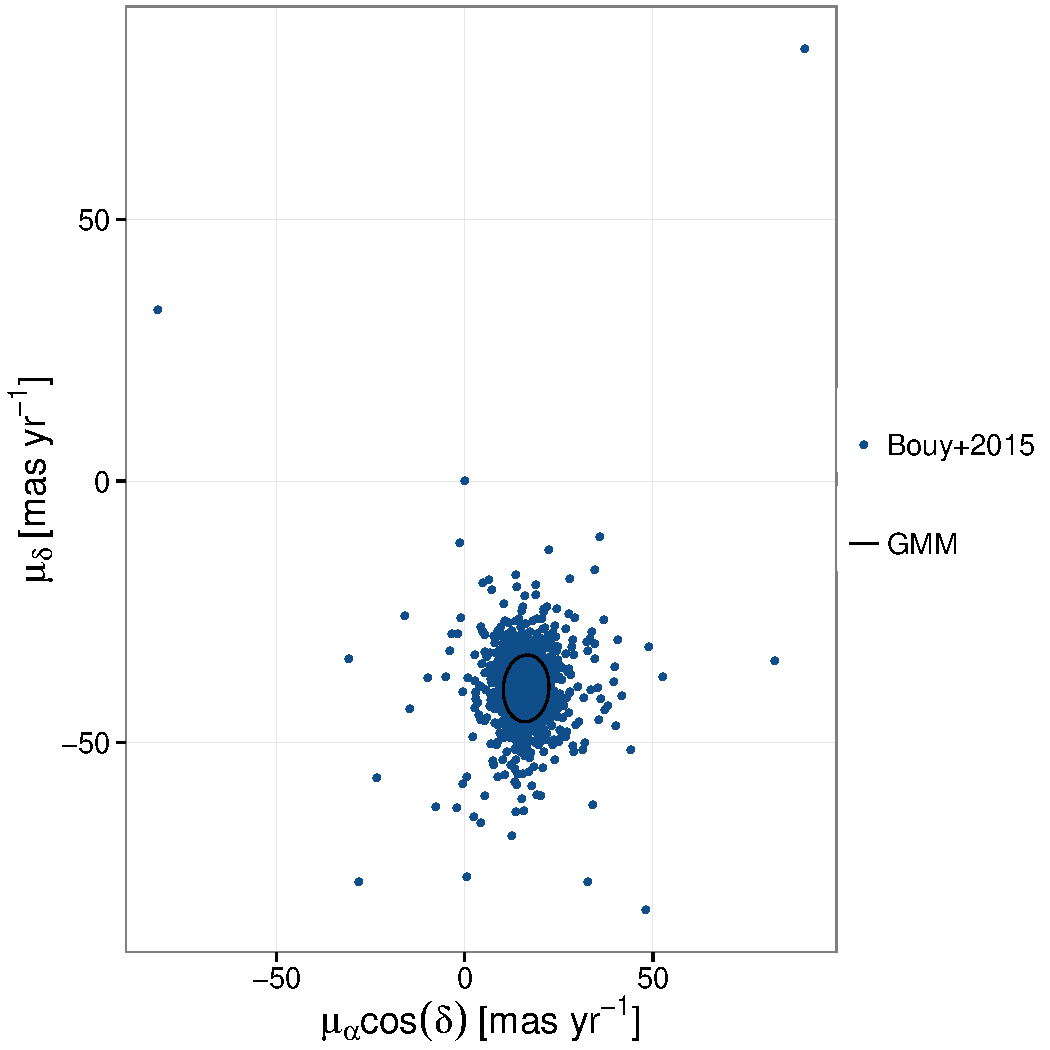
\includegraphics[page=1,width=\textwidth]{background/Figures/Hyp_PM_fit.pdf}
\caption{Proper motions of the candidate members of \citet{Bouy2015} in the \gls{rdr2} (blue dots), and fitted Gaussian (black line).}
\label{fig:fitPMone}
\end{figure}


As prior for the covariance matrices of both single stars and \gls{emb} proper motions we use the Half--$t(\nu,\mathbf{A})$ distribution. It is parametrised by a scalar $\nu$ and a vector $\mathbf{A}$. As shown by \citet{Huang2013}, this distribution family leads to more accurate estimations of covariance matrices than the traditional Inverse-Wishart distribution. In specific, the marginal correlation parameters, $\rho$, have the following distribution,

\begin{equation}
p(\rho) \propto (1-\rho^2)^{\frac{\nu}{2}-1}.
\end{equation}

The standard deviation term $\sigma_k$, associated to entry $k$, is distributed according to Half--$t(\nu,A_k)$. We set the hyper-parameters to $\nu=3$ and $\boldsymbol{A}_{pm}=\{10^5,10^5\}\,\mathrm{mas\cdot yr^{-1}}$. According to \citet{Huang2013}, arbitrarily large values of $\boldsymbol{A}$ lead to arbitrarily weakly informative priors on the corresponding standard deviation terms.

Concerning the photometric priors, they can be grouped in three categories: (i) priors for the the \emph{true} \gls{ci}, (ii) priors for the splines coefficients, and (iii) priors for the cluster sequence intrinsic dispersion. 

For the means in the univariate \gls{gmm} of the \emph{true} \gls{ci}, I choose a uniform distribution in the range  ($0.8\leq CI \leq8$). For the standard deviations I choose the Half--Cauchy$(0,\eta)$ distribution as suggested by \citet{Gelman2006}. The value of $\eta$ is set to an arbitrarily large value, $\eta=100$. Figure \ref{fig:priors_colour} shows the \gls{kde} of $10^3$ realisations from the prior distributions for the fractions, means, and variances of the parameters in the  \emph{true} \gls{ci} \gls{gmm}. Additonally, the lower right panel of this Fig. shows the resulting prior in the \gls{ci} space. Notice that values in this latter panel are truncated in the range of the observed \gls{ci}.

\begin{figure}[ht!]
    \centering
    \begin{subfigure}[t]{0.48\textwidth}
        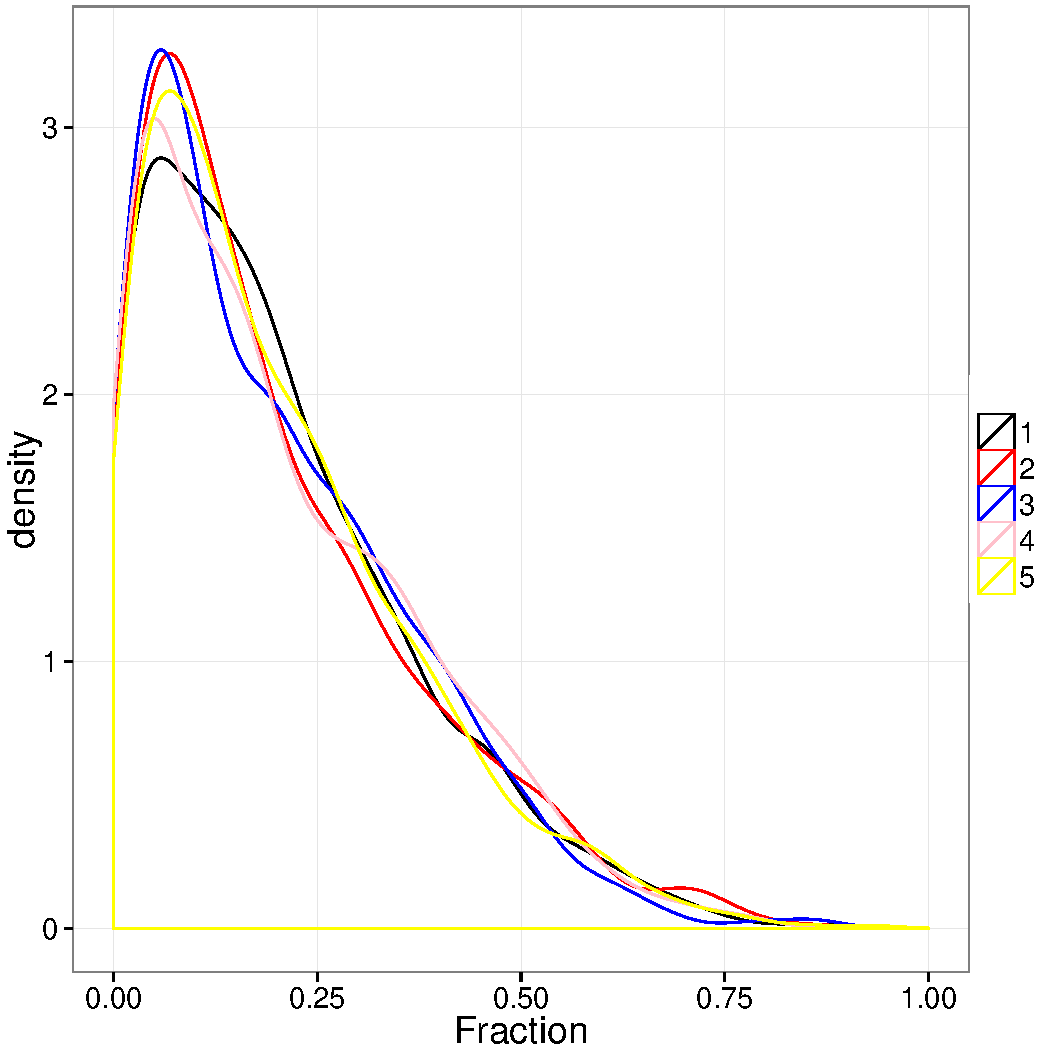
\includegraphics[page=1,height=9cm,width=\textwidth]{background/Figures/Priors_Color.pdf}
        \caption{}
    \end{subfigure}
    \begin{subfigure}[t]{0.48\textwidth}
      \includegraphics[page=2,height=9cm,width=\textwidth]{background/Figures/Priors_Color.pdf}
        \caption{}
    \end{subfigure}
     \begin{subfigure}[t]{0.48\textwidth}
      \includegraphics[page=3,height=9cm,width=\textwidth]{background/Figures/Priors_Color.pdf}
        \caption{}
    \end{subfigure}
     \begin{subfigure}[t]{0.48\textwidth}
      \includegraphics[page=4,height=9cm,width=\textwidth]{background/Figures/Priors_Color.pdf}
        \caption{}
    \end{subfigure}
\caption{\gls{kde} of $10^4$ realisations of the prior distributions of parameters in the \emph{true} \gls{ci} \gls{gmm}. Distributions of: (a) The field fraction $\pi$, (b) The \gls{emb} fraction, $1-\pi_{CB}$, (c) the proper motions cluster fractions, $\pi_{Cs}$, and (d) the proper motions equal-mass binaries fractions $\pi_{Bs}$.}
\label{fig:priors_colour}
\end{figure}

For the coefficients in the spline series we set the priors as univariate normal distributions. To find the mean and variance of these distributions we proceed as follows. First, we remove the \gls{emb} from the list of candidate members of \citet{Bouy2015}. To do this, I performed an iterative fit of the cluster sequence, at each iteration I removed those objects whose photometry was  as bright as that of the \gls{emb}. In the region of $CI > 7$ there are no candidate members of \citet{Bouy2015} or of any other source, see Fig \ref{fig:fitCMDs}. Thus, to provide a prior we complement our list of candidate members with the brown-dwarfs from the \citet{Faherty2012} sample. We choose only those objects observed in the same photometric bands of our data set. Finally, we fit the splines, and use the coefficients of this fit as the means, $\mu_{\beta}$ of the univariate normal distributions. \textbf{Figure \ref{fig:fitCMDsBD} shows the four cubic \glspl{bspline} fitted to our four \glspl{cmd} complemented with the \glspl{bd} of \citet{Faherty2012}}. The standard deviation terms were set to $\sigma_{\beta}=\{1,1,1,1,1,0.5,0.1\}\,\mathrm{mag}$. These values provide a reasonable compromise between cluster sequences compatible with the previously known candidates, and those far away or with exotic shapes. We show a sample of these priors in Fig. \ref{figure:priorcoefs}. This Figure shows also the brown-dwarfs from \citet{Faherty2012} and the sequence (dashed line) we use to provide the means of the univariate normal distributions.

\begin{figure}[ht!]
    \centering
    \begin{subfigure}[t]{0.48\textwidth}
        \includegraphics[page=2,height=8cm,width=\textwidth]{background/Figures/Photometry_fit.pdf}
        \caption{}
    \end{subfigure}
    \begin{subfigure}[t]{0.48\textwidth}
      \includegraphics[page=4,height=8cm,width=\textwidth]{background/Figures/Photometry_fit.pdf}
        \caption{}
    \end{subfigure}
     \begin{subfigure}[t]{0.48\textwidth}
      \includegraphics[page=6,height=8cm,width=\textwidth]{background/Figures/Photometry_fit.pdf}
        \caption{}   
    \end{subfigure}
     \begin{subfigure}[t]{0.48\textwidth}
      \includegraphics[page=8,height=8cm,width=\textwidth]{background/Figures/Photometry_fit.pdf}
        \caption{}
    \end{subfigure}
\caption{Spline fits (dashed lines) to the single stars candidate members of \citet{Bouy2015} (blue circles) and the \glspl{bd} of \citet{Faherty2012} (red crosses).}
\label{fig:fitCMDsBD}
\end{figure}


Again, I choose again the Half--t$(\nu,\boldsymbol{A})$ distribution to set the prior for the parameters of the cluster intrinsic dispersion, $\Sigma_{clus}$.  However, this time I use  $\boldsymbol{A}_{ph}=\{10,10,10,10,10\}$ mag. These values are large when compared to the standard deviation terms of the observed uncertainties. Therefore, they provide a weakly informative prior on the marginal standard deviation terms of the $\Sigma_{clus}$ covariance matrix.

Table \ref{table:hyperparameters} shows a summary all the hyper-parameter values used for the prior distributions. {Since the majority of these values come from the work of \citet{Bouy2015}, it is reasonable to question the influence that this particular work has on the results of the present one.}

{The methodology of the Bayesian Hierarchical Models, the one chosen here, has been specifically designed to avoid as much as possible the subjectivity of the chosen priors \citep{Gelman2006}. Thus, by using the results of \citet{Bouy2015} to set only the hyper-parameter values of the prior distributions we avoid much of the subjectivity of choosing that particular work. On top of that, the use of the weakly informative priors (see Section \ref{sect:generalities}) further decreases the impact of the prior information on the recovered posterior distributions.}

{Despite the weakly informative priors and the \gls{bhm} methodology, the work of \citet{Bouy2015} may have influence our results in a similar way as it was influenced by previous works. There is an unavoidable influence from the past into the present. In this work, we aim at keeping this influence at minimum by using the least subjective approaches to the inference process under a Bayesian framework.}

{Furthermore, as mentioned at the end of Section \ref{sect:generalities}, the prior information must be analysed in terms of the posterior distribution and verify if they make sense \citep{Gelman2006,Gelman2013}. Details of this analysis will be presented in Section \ref{sect:updating_priors}.}

{The quantitative analysis of the influence that the work of \citet{Bouy2015} may have in the present one should wait until further evidence (the application of the present methodology to other star clusters) is collected.}
 
\input{background/Tables/HyperParameters.txt}

\begin{figure}[ht!]
\begin{center}
\includegraphics[page=4,width=\textwidth]{background/Figures/Priors_Coefs.pdf}
\caption{\gls{cmd} $K_s$ vs. $i-K_s$ showing a sample (100 elements) of the prior for the coefficients in the splines series. Also shown are the brown-dwarfs from \citet{Faherty2012} sample (red dots), the cluster sequence (dashed line) used as mean for the priors, the candidate members of \citet{Bouy2015} (blue triangles), and a sample of the field (grey dots).}
\label{figure:priorcoefs}
\end{center}
\end{figure}

\section{Sampling the posterior distribution}

Theoretically, there are at least three possible approaches to obtain the posterior distributions of the parameters in our model. One of these options is the analytical approach. {The computing of the posterior distribution will become intractable given the size of the data set and the high dimensionality of the parametric space; the \gls{bhm} has 85 parameters}. The second option is the use of a grid in the parametric space. The likelihood and the prior must be evaluated at each point in this grid and then multiplied. This approach is reasonable when the parametric space is of moderate dimension ($\leq 5$). It requires the evaluation of the posterior distribution $q^p$ times, with $q$ the number of grid points in one dimension, and $p$ the dimension of the parametric space. The number of parameters in our model is 85, which immediately rules out this possibility. The third and so far only feasible approach is the use of \gls{mcmc} sampling methods. Although these methods provide a solution in a reasonable time, nevertheless, the bottle neck of computing time is due to the evaluation of the likelihood, which grows linearly with the size of the data set. 

This Section is structured as follows. First, I introduce an heuristic technique to perform a fast search of the maximum a posteriori of our target distribution. Then, I describe the \gls{mcmc} techniques available in the literature.{ In particular, I focus on the one technique we choose, and the reasons of this decision}. The Section ends detailing the convergence assessment of the \gls{mcmc}.

\subsection{PSO}

The likelihood of the data is the product of the individual likelihoods of each datum (Eq. \ref{eq:lik_datum}). Therefore, the number of operations needed to evaluate the likelihood grows proportionally to the size of the data. As I will explain in Section \ref{sect:MCMC}, the burn-in phase of \gls{mcmc} techniques allows them to reach the target distribution. However, once the \gls{mcmc} reaches this target distribution, the burn-in computations are discarded. Since the evaluation of the likelihood, and therefore of the posterior, is computationally expensive, I decided to reduce as much as possible the burn-in phase. To do so, I provide \gls{mcmc} with a set of initial solutions which are close to the \gls{map} of the target (posterior) distribution. These near-\gls{map} solutions must not be too crowded on the \gls{map}, or otherwise the \gls{mcmc} will spend too much time expanding them to reach the entire distribution. Here, there is a trade-off between the crowdedness of the solutions and its proximity to the \gls{map}. Since we aim at obtaining a representative sample of the posterior distribution and not just an estimate of it, then the initial set of solution for the \gls{mcmc} must be carefully chosen to minimise the computing time. This section provides the details of this procedure. 

{In Section \ref{sect:MCMC}, I will also show that the \gls{mcmc} flavour more suitable to our objective belongs to the family of \emph{ensemble} \gls{mcmc}. This flavour works with particles in the parametric space. To make the transition between the initial near-\gls{map} solutions and the  \gls{mcmc} particles as efficient as possible, I choose the \gls{pso} of  \citet{Kennedy1995}, which is a function optimiser that also works with particles. It provides a heuristic cheap-and-fast approach to the \gls{map} solution. The \gls{pso} works with an ensemble of particles which move through the parametric space.} These particles use the collective and individual past and present information to update their position. This information is specified by the score function, which in our case is the posterior distribution. The particles update their position iteratively according to their velocity. This velocity has a random but restricted magnitude. However, its direction is determined by the particle position, and the individual and collective positions with maximum score. \citet{Kennedy1995} show detailed description of the original algorithm, while a more efficient version is given by \citep{Clerc2002}.

Although the \gls{pso} is a simple and rather efficient solution to the \gls{map} approximation, it is far from perfect. Due to its heuristic origin, there is no theory behind its formulation. Furthermore, it does not guarantee the finding of the global maximum \cite[for a convergence guaranteed version see][]{Patel2013}. Although,  this issue does not affect our results (as we will see \gls{mcmc} does guarantee the finding of the target distribution once it has converged), it impacts the computing time. If the global maximum is not found in the \gls{pso} stage, then the \gls{mcmc} will take longer to arrive to the target distribution. 

On the other hand, the \gls{pso} stops its computations once the mean of the particles scores lies within a user defined tolerance. If this tolerance is too large, the \gls{pso} may stop far from the \gls{map}. If it is too small, it may converge to the \gls{map} but deliver solutions highly concentrated around it. This poses a problem to the following \gls{mcmc} stage. For it to explore the full posterior distribution, the \gls{mcmc} will need more iterations, thus more time, to expand the initially concentrated positions. {The optimal value for the relative tolerance is $10^{-7}$. I found it after several trials and errors. It was a time consuming exercise that will be avoided in the analyses of other clusters.} 

To overcome the problem of crowdedness, I decide to use the charged \gls{pso} \citep{Blackwell2002}. Originally designed to optimise a time varying score function, the charged \gls{pso} maintains its exploratory capabilities due to an electrostatic force that repels particles when they get closer than a certain distance \citep{Blackwell2002}. Thanks to this electrostatic force the charged \gls{pso} avoids the over-crowding of particles around local best values.

The algorithm of \citet{Blackwell2002} computes distances in the entire parametric space. I find this approach unsuitable for our problem, thus I modified it. {This modified version and the values chosen for its parameters are described with more detail in Section \ref{sect:code}, together with the rest of the developed codes. }

\subsection{MCMC}
\label{sect:MCMC}
\subsubsection{Generalities}
\glsfirst{mcmc} is the generic name for a series of algorithms whose objective is the sampling of probability distributions. As their name indicates, the \gls{mcmc} generates a chain (or a group of them) of Monte Carlo realisations that fulfil the Markov property. Monte Carlo realisations can be understood, broadly speaking, as continuous random realisations. Since it is an iterative algorithm, the chain is a process that refers to the joint of all random Monte Carlo steps. The Markov property indicates the probabilistic independence between steps in the chain that are separated more than one iteration. Thus, in a Markov chain, the probability of a future step depends only on the present step, and not in the past steps.

\citet{Andrieu2003} provides a brief and interesting summary of the history of the \gls{mcmc} methods. In the following I use their work to describe the fundaments of \gls{mcmc}. For more details, see the aforementioned authors and the book of \citet{Brooks2011}.

A stochastic process is defined as a sequence  $\{\theta_1,...,\theta_n\}$ of random elements. On it, each element $\theta_i \subset \mathbb{R}^k$,  with $k$ the dimension of the \emph{state space}. 

A stochastic process, $\boldsymbol{\theta}=\{\theta_0,\theta_1,...,\theta_n,\theta_{n+1}\}$ is called a Markov chain if
\begin{equation}
p(\theta_{n+1} | \theta_0,\theta_1,...\theta_n) = p(\theta_{n+1} |\theta_n). \nonumber
\end{equation}

A Markov chain has two important distributions, the initial distribution and the transition distribution. The initial distribution is the marginal distribution of $\theta_0$, $p(\theta_0)$. The transition distribution is the conditional probability $p(\theta_{n+1} |\theta_n)$. The latter is called stationary or homogeneous if it does not depend on $n$.

{If this transition is irreducible and aperiodic, then there is an \emph{invariant} or \emph{equilibrium} distribution to which the chain converges, regardless of the initial distribution. Here, aperiodic means that the chain does not have loops, while it is irreducible if the probability of exploring all other states is not zero.}

If we want to have $p(\theta)$ as the invariant distribution, then it suffices that the transition distribution $p_t(\cdot | \cdot)$ satisfies the detailed balance condition,
\begin{equation}
\label{eq:detailedbalance}
p(\theta_{n})\cdot p_t(\theta_{n-1}|\theta_n)=p(\theta_{n-1})\cdot p_t(\theta_n | \theta_{n-1}).
\end{equation}

Thus, \gls{mcmc} are Markov chains that satisfy the detailed balance condition, and have their invariant distribution as the target distribution. 
The large variety of \gls{mcmc} algorithms arises from the efficiencies with which they arrive to the target distribution.

In the following I will review three of the \gls{mcmc} categories: \gls{mh}, \gls{hmc} and affine invariant samplers. The \gls{mh} category comprises the classic \gls{mh} algorithm but also contain particular cases like the Gibbs sampler \citep{Geman1984}. I describe \gls{mh} only for completeness and explanatory reasons. Later, I will focus on the particular cases of \gls{hmc}, and affine invariant for ensemble samplers. Finally, I will briefly describe Nested Sampling, an algorithm that uses \gls{mcmc} to numerically compute the Bayesian evidence and simultaneously generate samples of the posterior distribution. 
\subsubsection{Metropolis-Hastings}
By far, the most popular \gls{mcmc} algorithm is Metropolis-Hastings \citep{Metropolis1953,Hastings1970}. Once the Markov chain has been initialised in the state space, given the current $\theta$ and the proposed $\hat{\theta}$ positions, the chain moves from $\theta$ to $\hat{\theta}$ with acceptance probability:

\begin{equation}
\mathcal{A}(\hat{\theta}|\theta)=min\left\{1,\frac{p(\hat{\theta})\cdot q(\theta|\hat{\theta})}{p(\theta)\cdot q(\hat{\theta}|\theta)}\right\},
\end{equation}
where $q$ is the transition probability. Since the algorithm allows rejection, it is aperiodic, and to ensure irreducibility, the support of $q$ must include that of $p$ \citep{Andrieu2003}. The popularity of \gls{mh} lies in its simplicity. Nevertheless it requires a careful tuning of the transition probability. Usually, this probability is given by a normal distribution. It works well for relatively low dimensions of the parametric space ($\leq 5$). However, once the dimension goes higher, the \gls{mh} algorithm spends a great amount of time tuning the parameters of this multivariate normal distribution. In particular, those of its covariance matrix.

\subsubsection{Hamiltonian Monte Calro}
The \glsfirst{hmc} algorithms \citep{Duane1987,Neal1996}, as their name suggest\footnote{Originally called Hybrid Monte Carlo by \citep{Duane1987}}, use Hamiltonian dynamics to express the target distribution as the potential distribution of a hamiltonian system of particles. In such systems the total energy is the sum of the potential and kinetic energies. The potential distribution depends only on position, whereas the kinetic one on momentum. \gls{hmc} introduces a momentum to the particles in order to use their positions as a sample of the target distribution. To update the particles positions, \gls{hmc} uses the Hamilton equations, which contain information about the gradient of the potential. Once \gls{hmc} has tuned the momentum distribution, the proposed positions are more likely in terms of the target distribution. Therefore, using the information about the gradient of the target distribution, \gls{hmc} is able to improve the acceptance ratio of the proposed steps. A detailed description of \gls{hmc} can be found in Chapter 5 of \citet{Brooks2011}. The package \emph{Stan} \citep{Stan} provides an efficient implementation of \gls{hmc}.

\subsubsection{Affine invariant}
Affine invariant \gls{mcmc} samplers use many particles, the ensemble, to sample the target distribution with a performance that is independent of its shape in the parametric space. Affine invariant \gls{mcmc} does not need the tuning the transition probability. For this reason, these samplers are faster than standard \gls{mcmc} \citep{Goodman2010}. In the following I use the derivation of \citet{Goodman2010}.


{An ensemble $\boldsymbol{\theta}$ is a set of $L$ particles $\theta_l \subset \mathbb{R}^k$. It lives in state space $\mathbb{R}^{kL}$, and the positions of it particles are independently drawn from the target distribution $\pi$.} Therefore,

\begin{equation}
\Pi(\boldsymbol{\theta})=\pi(\theta_1)\cdot\pi(\theta_2)...\pi(\theta_L).\nonumber 
\end{equation}

Thus, an ensemble \gls{mcmc} is a Markov chain in the state space of ensembles. An ensemble \gls{mcmc} preserves the equilibrium distribution without the individual particles sequence, $\theta_1(1),\theta_1(2),...\theta_1(t)$, being Markov or even independent. However, to update the particles positions, the detailed balance condition (Eq. \ref{eq:detailedbalance}) must be fulfilled. \citet{Goodman2010} use partial resampling to ensure this. In partial resampling, the transition probability preserves the target (invariant) distribution if the single particle steps preserve the conditional distribution of the particle position given the complementary ensemble (the rest of the particles). Using the affine invariant \emph{stretch move} (see below), these authors are able to define a Markov chain, in the state space of ensembles, that satisfies the detailed balance condition. 

The stretch move $\theta_k(t) \rightarrow \hat{\theta}$ is defined as,
\begin{equation}
\label{eq:stretchmove}
\hat{\theta}= \theta_j(t) + z\cdot(\theta_k(t)-\theta_j(t)),\nonumber 
\end{equation}
where $\theta_j(t)$ is the current position of a particle in the complementary ensemble, and $z$ is the stretching factor. It produces a symmetric transition, $p(\theta_k(t) \rightarrow \hat{\theta})=p(\theta_k(t) \leftarrow \hat{\theta})$, if its density $g(z)$ satisfies the symmetry condition
\begin{equation}
g(\frac{1}{z})= z\cdot g(z).\nonumber 
\end{equation}
Finally, \citet{Goodman2010} define their affine invariant \gls{mcmc} using the following distribution for $g(z)$,

\begin{equation}
g(z) \propto \left\{ \begin{array}{rcl}
         \frac{1}{\sqrt{z}} & \mbox{for}&  z\in[1/a,a] \\ 
         0  & \mbox{for} &  z\notin[1/a,a]
                \end{array}\right.
\label{eq:gz}
\end{equation} 
and the acceptance probability,

\begin{equation}
\mathcal{A}(\hat{\theta}|\theta)=min\left\{1,z^{n-1}\cdot \frac{p(\hat{\theta})}{p(\theta)}\right\}.
\end{equation} 

{The parameter $a$, which must be greater than one, improves the performance of the sampler \citep{Goodman2010}. The acceptance fraction of the proposed transitions depends both on the ratio of probabilities $p(\hat{\theta})/p(\theta)$ and on the value of $z^{n-1}$. The support of the latter depends on the parameter $a$. Given $g(z)$ and certain dimension of the parametric space, increasing $a$ results in more probable smaller values of $z$, thus in smaller acceptance probabilities.}

One of the great advantages of \gls{mcmc} ensemble samplers  is its possibility of parallelisation. Since they work with particles, these particles can be distributed among cores in a computer cluster, therefore reducing the computing time when compared to non ensemble \gls{mcmc}. \citet{Foreman2013} implemented the affine invariant stretch move of \citet{Goodman2010} in the Python package \emph{emcee}. 
\subsubsection{Nested sampling}
\label{sect:NestedSampling}
Nested sampling \citep{Skilling2004,Skilling2006} is an algorithm designed to numerically integrate the evidence (Eq. \ref{eq:evidence2}). As a by-product, it also delivers a sample of the posterior distribution. 

{To compute the evidence integral, it uses $N$ particles whose positions, in the parametric space, are sampled from the prior. Then, at each subsequent step $i$ the algorithm computes the likelihoods of the $N$ particles. The particle with lowest likelihood is stored as $x_i$ together with its likelihood $L_{i}$. The weight $w_i$ is computed as}
\begin{equation}
w_i = e^{-\frac{(i-1)}{N}} - e^{-\frac{i}{N}}. \nonumber 
\end{equation}
{The particle $x_i$ is replaced with a new draw from the prior, on the condition that its likelihood is greater than $L_i$. }

{Once certain number of iterations have been done, the evidence integral is approximated by 
}\begin{equation}
z \leftarrow \sum_i w_i\cdot L_i.
\end{equation}

{The original algorithm was designed to compute the evidence of a unimodal distribution. However, an improved version of the original algorithm was implemented in \emph{MultiNest} \citep{Feroz2009}. This version allows the sampling and computing of evidence in the even more difficult multimodal posteriors.  }

\subsection{Implementation and convergence: PSO and MCMC}
To sample the posterior distribution in our problem, we choose \emph{emcee} due to the following properties: i) the affine invariance allows a faster convergence over common and skewed distributions \cite[see][for details]{Goodman2010,Foreman2013}, ii) it can be run in parallel by distributing particles over the nodes of a computer cluster, which reduces considerably the computing time; and iii) it requires the hand-tuning of only two constants: the number of particles, and the parameter $a$ of the $g(z)$ distribution(Eq. \ref{eq:gz}). I choose a ratio of particles to parameters of two, that results in 170 particles. This is the minimum ratio recommended by \citet{Foreman2013}, which still allows a reasonable computing time. After trial and error, I fix the value of the $a$ parameter to $a=1.3$. As mentioned by \citet{Goodman2010}, this parameter can be tuned to improve performance of the sampler. This value keeps the acceptance fraction in the range $0.2-0.5$, as recommended by \citet{Foreman2013}.

{As a front-end of \emph{emcee}, and to handle the input and output of data, I use a modified version of the \emph{emcee} handler known as \emph{Cosmo Hammer} \citep{Akeret2013}. The next Section provides the details of these modifications. }

As mentioned earlier, the \gls{pso} does not guarantee the finding of the global maximum of the score function. Therefore, I implement an iterative approach that minimises the risk of the \gls{pso} getting stuck in local maxima. To do so, I iteratively run \gls{pso} and 50 iterations of \emph{emcee} (with the same number of particles as the \gls{pso}) until the relative difference between means of consecutive iterations is lower than $10^{-7}$. The iterations of \emph{emcee} spread the \gls{pso} solution without moving away from the target distribution. 
 
Neither scheme, \gls{pso} alone or \gls{pso}-\emph{emcee}, guarantees finding the global maximum. The solution this scheme provides could indeed be biased. However, we use them to obtain only a fast estimate of the global maximum, or at least, of points in its vicinity. If the initial solution provided by this scheme is indeed biased, the final \emph{emcee} run erases, during the burning phase, any dependance on the initial solutions. After the convergence of the \gls{pso}-\emph{emcee} scheme, I run \emph{emcee} alone until it converges.  
 
Convergence to the target distribution occurs when each parameter enters into the stationary equilibrium or normal state. The Central Limit Theorem ensures that this state exists. See \citet{Roberts2004} for guaranteeing conditions and \citet{Goodman2010} for \emph{irreducibility} of the \emph{emcee} stretch move. The stationary or normal state is reached when, in at least 95\% of the iterations, the sample mean is bounded by two standard deviations of the sample, and the variance by the two standard deviation of the variance \footnote{
$sd(\sigma^2)=\sigma^2 \sqrt{\kappa/n + 2/(n-1)}$ with $\kappa$ the kurtosis and $n$ the sample size.
}. Fig. \ref{fig:convergence} shows the mean and variance of the ensemble of \emph{emcee} particles for the last 4000 iterations before stoping the sampling. Both the mean and variances are normalised to the value of the last iteration.


\begin{figure}[H]
    \centering
    \begin{subfigure}[t]{0.45\textwidth}
    \centering
        \includegraphics[width=\textwidth]{background/Figures/BHM/AllMeanParticles.pdf}
        \caption{}
    \end{subfigure}
    \begin{subfigure}[t]{0.45\textwidth}
    \centering
      \includegraphics[width=\textwidth]{background/Figures/BHM/AllVarParticles.pdf}
        \caption{}
    \end{subfigure}
\caption{Normalised mean (a) and variance (b) of each parameter in \gls{bhm} model as functions of iterations. The normalisation values are the mean and variance of the ensemble of particles positions at the last iteration. Red lines show one and two sigma levels of these normalisation values. Only shown the last 4000 iterations previous to stopping the algorithm.}
\label{fig:convergence}
\end{figure}


I stop the \emph{emcee} sampling once all parameters have entered the equilibrium state and the criterium of \citet{Gong2016} \footnote{Implemented in the R package \emph{mcmcse} \citep{mcmcse}} is fulfilled. We choose this criterium because it was developed for high-dimensional problems and tested on Hierarchical Bayesian Models, as in the present work. In this criterium, the \gls{mcmc} chain stops once its \gls{ess} is larger than a minimum sample size. This minimum is computed using the required accuracy, $\upsilon$, for each parameter confidence interval $(1-\delta)\cdot$100\%. The \gls{ess} is the size that an independent and identically distributed sample must have to provide the desired accuracy on the parametric inference. 

The \emph{emcee} run stops once the \gls{ess} of the ensemble of walkers is greater than the minimum sample size needed for the required accuracy $\epsilon = 0.05$ on the 68\% confidence interval ($\delta = 0.32$) of each parameter.


\section{Codes}
\label{sect:code}
This Section sets out the details about the code I developed to perform the computation described throughout this chapter. First, I give a brief chronological description of the model development. Later, I will describe the details on the implementation of the charged \gls{pso}, the modified \emph{emcee}, and the \gls{gmm} used to describe the field population. Finally, I will end this Section detailing the hybrid \gls{hpc} code developed to minimise the computing time of the posterior distribution in the \gls{bhm}.

The first version of the Bayesian Hierarchical Model was implemented by \'Angel Berihuete in the package \emph{Stan} \citep{Stan}. It comprised a Bayesian model of the \gls{mle} model of \citet{Sarro2014}. The proper motions were modelled using a single mixture of gaussians. The photometry was modelled with a Chebyshev polynomial parametrised by the length along the sequence. This length was found using a principal curve analysis and lacked physical interpretation.

I took this version and modified it in the following aspects. I included the photometric and proper motions \gls{emb} sequence, the uncertainties both in proper motion and in the photometry, and the width of the sequence modelled as the multivariate gaussian. Then, we realised that the principal curve analysis is not compatible with the deconvolution methodology. {The principal curve analysis finds the dominant curve in the observed data, and not the \emph{true} underlying relation that generates the observed data once the individual noise process for each object is accounted for. For this reason, the principal curve analysis is affected by individual uncertainties \cite[see][for the negative impact of heteroscedastic data on the related principal component analysis]{Hong2016}. Instead, we decided to model the intrinsic \emph{true} underlying photometric relation with polynomials. We use as parameter for these polynomials the \emph{true} colour \gls{ci}, which is a more interpretable parameter than the distance along the principal curve, which was used in the previous version. Since we have one \emph{true} \gls{ci} for each object, the number of parameters is equal to the number of objects. We marginalised all these nuisance parameters with the aid of a prior. For this prior we introduced a probability distribution modelled by a \gls{gmm}.}

Previous to the introduction of the marginalisation of the nuisance parameters, the model worked fine on samples of a few hundreds of stars. Once the marginalisation was introduced, the computing time of the model increased dramatically, rendering its application to higher data sizes impractical. At this point we decided to port the existing \emph{Stan} code into \emph
{Python}\footnote{https://www.python.org} so that we could work with the parallel \emph{emcee} code. \emph{emcee} proved to be of great use. Due to its parallelisation capabilities we were able to increase the data size from 2000 to 10,000 objects. Since the computing of the likelihood was the highest computational challenge, I developed my own routines to perform it in parallel. However, \emph{CosmoHammer} \citep{Akeret2013} turned out to be more efficient in distributing the parallel loads. I ported the \gls{bhm} code into \emph{CosmoHammer} and modified the latter. The modifications ranged from data files and log entries to the introduction of priors and the handling of a Hybrid-\gls{hpc} scheme using both \gls{mpi} and multithreading. Despite the Hybrid-\gls{hpc} scheme, the computing of the likelihood of a data set with $10^5$ objects seemed unreachable. At this point, I performed two tasks: the first was to strip the code of all auxiliary libraries calls, and the second was the vectorisation of the majority of the operations. Since the parameters of the field were held fixed, the field likelihood was computed externally for each object. The code was then fed with the data set, the field likelihood, and all the auxiliary computations reduced to a minimum. Among the reduced computation there are, for example, the Cholesky decompositions and matrix inversions of the covariance matrices of the uncertainty. Instead of doing these computation inside the code, the code was fed with the precomputed values. This further reduced the computing time.

Introducing \gls{pso} and later the charged \gls{pso} further reduced the computing time.  At this point the code was able to run on a data set with $10^5$ objects. However, convergence of the \gls{mcmc} still required several weeks of computations. Once the approximation to the marginalisation integral (Eqs. \ref{eq:clmarginalps} and \ref{eq:clmarginalpb}) was introduced, the computing time reduced far more. Finally, the tuning of the \emph{emcee} parameters allowed us to increase the acceptance fraction, and reach convergence within four weeks of full computing time with an 80 cores computer cluster. It is indeed a very long time. However it is reasonable compared with our original estimates of approximately 2 years of computing time\footnote{Today, the \gls{dance} team is working on a \gls{gpu} version of the code which computes the same amount of calculations in a couple of days.}.

\subsection{The modified charged PSO}
\label{sect:chargedPSO}
As explained before, the charged \gls{pso} of \citet{Blackwell2002} was inappropriate to our objective. The metric of the parametric space of our problem is not isotropic because parameters have different length scales. For example, while fractions are constrained in the $[0,1]$ interval, proper motions parameters are allowed in the range of proper motion measurements $[-99,99]\,\mathrm{mas\cdot yr^{-1}}$. Therefore, the use of an isotropic metric results in a solution which is crowded in some parameters while is over-dispersed in others. 
To solve this issue, I modified the charged \gls{pso} by measuring distance between particles and applying the electrostatic force independently on each parameter. In such a way, the electrostatic force plays a role only when the relative distance between particles in any given parameter is smaller than $10^{-10}$. I found this value heuristically.

In the original version of  \citet{Blackwell2002}, each particle is subject to the acceleration,
\begin{equation}
\label{eq:PSOacc}
\mathbf{a}=\sum_{i\neq j} \frac{q_i \cdot q_j }{r_{ij}^3} \cdot \mathbf{r}_{ij}, \ \ \ \ p_{core} < r_{ij} < p
\end{equation}
where $q_i$ and $q_j$ are the charges of particles $i$ and $j$, and $r_{ij}$ is the distance between them. The distances $p_{core}$ and $p$ indicate the minimum and maximum distances at which the electrostatic force comes into action. Outside this range, the electrostatic force is zero. In this equation, $\mathbf{r}_{ij}= \mathbf{x}_i -\mathbf{x}_j$, where $\mathbf{x}_i,\mathbf{x}_j$ are the positions of particles $i$ and $j$. Also, $\mathbf{r}_{ij},\mathbf{x}_i,\mathbf{x}_j \subset \mathbb{R}^d$, with $d$ the dimension of the space. 

In the modified version, the distance is measured independently in each dimension of the parametric space. Thus, $\mathbf{r}_{ij}= \{x_{1,i} -x_{1,j},x_{2,i} -x_{2,j},...,x_{d,i} -x_{d,j}\}$. Also the acceleration has the form,
\begin{equation}
\label{eq:PSOacc}
\mathbf{a}=\sum_{i\neq j} \frac{q_i \cdot q_j }{r_{ij}^2} \cdot \mathbf{r}_{ij}, \ \ \ \  10^{-50} < \frac{r_{ij}}{r_{eq}} < \epsilon
\end{equation}
and it is now applied over each dimension of the parametric space. The distance $r_{eq}$ is that at which the velocity caused by the acceleration equals the mean velocity caused by the common \gls{pso}. $\epsilon$ is a free parameter which, as said previously, was set heuristically to $10^{-10}$.

\subsection{Improvements of emcee}
The modification I introduced in \emph{emcee}, although very simple, improved the acceptance fraction and mixing of the particles.
To allow the parallelisation, \citet{Foreman2013} divide the ensemble of particles in two ensembles. In the original version, the particles in one ensemble use one and the same particle in the complementary ensemble to compute their positions according to Eq. \ref{eq:stretchmove}. In the modified version, particles from one ensemble update their positions using a particle from the complementary ensemble. However, this particle is chosen randomly at each iteration. 

In a private communication with Daniel Foreman-Mackey, the developer of \emph{emcee}, he mentions that a similar modification was already introduced in a beta version of the \emph{emcee} code.

%Figure \ref{fig:emcee\gls{dance}} compares the mixing and acceptance fractions of the original and modified versions of \emph{emcee}.
%\begin{figure}[htbp]
%\begin{center}
%%\includegraphics[width=\textwidth]{}
%\caption{Comparison between the log posterior evaluations of the original emcee version (left) and the modified one (right). }
%\label{fig:emceeDANCe}
%\end{center}
%\end{figure}
\subsection{GMM for the field population}
\label{sec:codeGMM}
As mentioned earlier in this Chapter, the field population is modelled by means of two independent photometric and proper motion distributions. The \gls{mle} of the parameters of these distributions were found using the \gls{em} algorithm.  The conventional \gls{em} algorithm for \gls{gmm} \citep{Dempster1977} for a mixture of $M$ gaussians goes as follows. Given a set of parameters $\theta=\{w_i,\boldsymbol{\mu}_i,\boldsymbol{\Sigma}_i\}_{i=1}^M$, were $w_i$,$\boldsymbol{\mu}_i$, and $\boldsymbol{\Sigma}_i$ are the fraction, mean and covariance matrix of gaussian component $i$, the likelihood of the data is,

\begin{equation}
p(\{\mathbf{y}_n\}_{n=1}^N|\theta)=\prod_{n=1}^N {\sum_{i=1} ^M {w_i\cdot \mathcal{N}(\mathbf{y}_n|\boldsymbol{\mu}_i,\boldsymbol{\Sigma}_i)}}.
\end{equation}

To solve the problem, the \gls{em} algorithm requires  a set of $N$ variables, $\{\boldsymbol{z}_n\}_{n=1}^N$, of dimension $M$. The variable $z_{n,i}$ represent the probability that observation $y_n$ was drawn from gaussian $i$. Therefore,

\begin{equation}
1=\sum_{i=1}^M z_{n,i}.
\end{equation}

These $\boldsymbol{z}$ latent variables are found as
\begin{equation}
z_{n,i}= \frac{w_i\cdot \mathcal{N}(\mathbf{y}_n|\boldsymbol{\mu}_i,\boldsymbol{\Sigma}_i)}{\sum_{i=1}^M w_i\cdot \mathcal{N}(\mathbf{y}_n|\boldsymbol{\mu}_i,\boldsymbol{\Sigma}_i)}.
\end{equation}

The \gls{em} works, as its name indicates, by maximising the expected value of the likelihood. The latter is given by
\begin{equation}
E[p(\{\mathbf{y}_n\}_{n=1}^N|\theta)]=\prod_{n=1}^N {\sum_{i=1} ^M {z_{n,i}\cdot w_i\cdot \mathcal{N}(\mathbf{y}_n|\boldsymbol{\mu}_i,\boldsymbol{\Sigma}_i)}}.
\end{equation}

The previous expectation is maximal when,
\begin{align}
w_i &= \frac{1}{N} \sum_{n=1}^N z_{n,i}, \\
\boldsymbol{\mu}_i &= \frac{1}{\sum_{n=1}^N z_{n,i}} \sum_{n=1}^N z_{n,i}\cdot \mathbf{y}_n,\\
\boldsymbol{\Sigma}_i &= \frac{1}{\sum_{n=1}^N z_{n,i}} \sum_{n=1}^N z_{n,i}\cdot (\mathbf{y}_n - \boldsymbol{\mu}_i)\times(\mathbf{y}_n-\boldsymbol{\mu}_i)^T.
\end{align}

The modified version of the \gls{gmm}, which includes a uniform distribution, is now a particular case of the \gls{gmm}. This can be viewed as a gaussian distribution with fixed parameters and a constant probability $c$ given by the uniform distribution. The new expectation is then,
\begin{equation}
E[p(\{\mathbf{y}_n\}_{n=1}^N|\theta)]=\prod_{n=1}^N {\left[z_{n,0}\cdot w_0 \cdot c + \sum_{i=1} ^M {z_{n,i}\cdot w_i\cdot \mathcal{N}(\mathbf{y}_n|\boldsymbol{\mu}_i,\boldsymbol{\Sigma}_i)}\right]}.
\end{equation}

The maximisation step remains identical except for the indices. There are now $M+1$ fractions $w_i$, with $i=0,1,...,M$, and the means and covariances run from $i=1,...,M$.

Regarding the photometric \gls{gmm} of the field, and given that the photometry has missing values, we use the \gls{em} algorithm of \citet{McMichael1996}. This algorithm was developed to obtain the \gls{mle} of data sets containing objects with missing values. A recent and faster version was developed by \citet{Lin2006}. Although this new version is faster, its mean absolute relative error is in the range 0.02-0.2 (see Tables2 and 3 of the mentioned authors). In \citet{McMichael1996} algorithm this indicator is lower, at least for fractions and means (see Fig. \ref{fig:validate_MGMM}).

In the algorithm of \citet{McMichael1996}, there is a set of $N$ gain matrices, one for each datum. Each $M_n$ matrix is an identity matrix in which the rows of the corresponding missing value have been deleted. Thus, the expected value of the likelihood is now,

\begin{equation}
E[p(\{\mathbf{y}_n\}_{n=1}^N|\theta)]=\prod_{n=1}^N {\sum_{i=1} ^M {z_{n,i}\cdot w_i\cdot \mathcal{N}(\mathbf{y}_n|M_n \boldsymbol{\mu}_i,M_n\boldsymbol{\Sigma}_i M_n)}}.
\end{equation}

The maximisation step is now,

\begin{align}
w_i &= \frac{1}{N} \sum_{n=1}^N z_{n,i}, \\
\boldsymbol{\mu}_i &= \frac{ \sum_{n=1}^N z_{n,i}\cdot H_n \mathbf{y}_n}{\sum_{n=1}^N z_{n,i} H_n M_n}
\end{align}
with 
\begin{equation}
H_i=M_i^T(M\Sigma_i M^T)^{-1}
\end{equation}

The maximisation step has no analytical solution for the covariance matrix. Therefore, a modified steepest descent is used

\begin{equation}
\Sigma_i \leftarrow \Sigma_i + \frac{\rho}{2}\cdot \Sigma_i\Delta_i\Sigma_i,
\end{equation}
with $\Delta_i$ given by

\begin{equation}
\Delta_i=  \frac{1}{\sum_{n=1}^N z_{n,i}}\cdot \sum_{n=1}^N z_{n,i} \cdot \left[H_n(\mathbf{y}_n -  M_n \boldsymbol{\mu}_i) \times  (\mathbf{y}_n -  M_n \boldsymbol{\mu}_i)^TH_n^T - H_nI\right].
\end{equation}
 
 This algorithm preserves the monotonic convergence of the conventional \gls{em}, and returns positive definite matrices provided that $\rho < 2$. For details and validation of this algorithm see \citet{McMichael1996}. \textbf{Nevertheless, I tested the validity of this algorithm on synthetic data sets. I created them using the parameters of the photometric model presented in Section \ref{sect:field_population}.  Figure \ref{fig:validate_MGMM} shows the mean absolute relative differences between each of the input and recovered parameters in the \gls{gmm}. The panels are separated by the kind of parameter: fractions, means and covariance matrices. The mean absolute relative differences are shown as a function of the sample size and the fraction of objects with missing values. The latter were randomly chosen, with missing entries in three of the five observables. As can be seen from this figure, the algorithm performs reasonably well in the explored range of sample sizes and missing fractions.}
 
 \begin{figure}[H]
    \centering
        \includegraphics[width=\textwidth]{background/Figures/Analysis_Missing_GMM.pdf}
\caption{Mean of the relative difference between the input parameters and the recovered ones as a function of the sample size and the fraction of objects with missing values.}
\label{fig:validate_MGMM}
\end{figure}


\subsection{Hybrid-HPC implementations}
\label{sect:HHPC}
As I outlined before, the parallel computing approach was an unavoidable step. Once the code was ported to \emph{Python} and \emph{CosmoHammer}, I modified the latter to better fit our needs. The modifications were mainly on the management of input and output files and the python \emph{multiprocessing} package for the multithreaded computing of likelihoods. Also, I striped some of its original functions to reduce memory usage and implemented some others, like the use of initial positions for the particles.

In the Hybrid-\gls{hpc} approach, the particles of \emph{emcee} are distributed on the nodes of the computing cluster by means of the \gls{mpi} protocol. Then, each core in the node computes the likelihood of one fraction of the objects in the data set. This Hybrid-\gls{hpc} code was implemented and tested in different computing cluster architectures. For the cluster at the Centre of Astrobiology (Villanueva de la ca\~nada, Madrid, Spain), I used a configuration of 6 nodes each with 12 cores. For the cluster at the University of C\'adiz, (Andalucía, Spain) I used a configuration of 5 nodes each with 16 cores.

However, the  Hybrid-\gls{hpc} approach was not the best solution at the Infrastructure de Calcul Intensive et de Donées\footnote{https://gricad.univ-grenoble-alpes.fr}of the University of Grenoble Alpes. At the Froggy\footnote{https://ciment.ujf-grenoble.fr/wiki-pub/index.php/Hardware:Froggy} cluster, the code continuously render errors of communication. For this reason, I implemented a \gls{mpi}-only version of the code. In this version, the multithreading approach is left aside. Instead, the totality of the available cores is fully dedicated to the computing of the likelihood. Each of the $n$ cores computes the likelihood of the $n$th fraction of the objects in the data set. Once the likelihood of all particles has been computed, the master node evaluates the new positions of the particles.

I finish this chapter with a brief description of the difficulties faced in the development and testing of the \gls{bhm} code. As the code evolved in complexity, my computational skills were compelled to evolve as well. I started by learning R and solving some toy problems on it. Later, when the dimensionality of the posterior increased I learned \emph{Stan}. When the data set increased in size, we faced the parallelisation, so I learned Python and \gls{mpi}. Once these versions were operable, I was forced to deal with libraries, from the common, numpy, scipy and numba, to the linking of modules and libraries. Finally, when dealing with several clusters I learned the queue languages Condor, slurm and OAR. Currently, I am working on the improvement (memory allocation and data distribution) of the \gls{gpu} implementation of the \gls{bhm} code.  

\section{The methodology for the analysis of the PSD}
\label{sect:PSDmethod}

In this Section, I present the methodology used to investigate the \glsfirst{psd} of the Pleiades. As explained in Section \ref{sect:RF-2}, we do an independent analysis of the \gls{psd} and the photometric and kinematic (proper motions) distributions (the reasons for this decision are detailed in the mentioned section). The data set for this analysis is the one called the \gls{t+d}, which is described in Section \ref{sect:Tycho+DANCe}. Here suffices to mention that it comprises the largest and less contaminated sample of Pleiades candidate members to date.  Although the analysis of the \gls{psd} uses the membership probabilities inferred by the \gls{bhm} (at Chapter \ref{chap:Results}), and those derived by \citet{Bouy2015} for the Tycho-2 sample, it is independent of them because in both analyses the sky positions are explicitly removed. 

The generative model of the \gls{psd} is similar to that of the \gls{bhm}  (Eq. \ref{eq:genmod}). However, instead of inferring the fraction of field objects in the data set (which would be similar to the estimated contamination rate, see Section \ref{sect:TDContamination}), each object contributes to the cluster model proportionally to its cluster membership probability, $P$. Thus the generative model of the \gls{psd} for object $n$ is

\begin{equation}
\label{eq:genmodPSD}
p(\mathbf{d}_n,P_n |\boldsymbol{\theta}_c,\boldsymbol{\theta}_f)=(1-P_n) \cdot p_f(\mathbf{d}_n|\boldsymbol{\theta}_f) + P_n\cdot p_c(\mathbf{d}_n| \boldsymbol{\theta}_c),
\end{equation}

with $\mathbf{d}_n$ the vector of observations, comprising the sky positions ($\alpha$ and $\delta$), the photometric band $J$, and $P_n$  the cluster membership probability. The terms $p_f(\mathbf{d}_n|\boldsymbol{\theta}_f)$ and $p_c(\mathbf{d}_n|\boldsymbol{\theta}_c)$ are the field and cluster likelihood, respectively, of the datum $\mathbf{d}_n$ given the field, $\boldsymbol{\theta}_f$ and cluster, $\boldsymbol{\theta}_c$, parameters. Since all objects in the \gls{t+d} have R.A. and Dec. uncertainties which are symmetric, almost identical (homoscedastic uncertainties), and negligible ($\sim 2\times10^{-6}$ deg) compared to the size of the cluster ($\sim7^{\circ}$), we can safely assume that: i) the data are independent and identically distributed, and ii) the observed positions correspond to the \emph{true} ones. Thus, the uncertainties are not included in the generative model. 

We assume that the contaminants ($\sim 8\%$, see Section \ref{sect:Tycho+DANCe}) in the \gls{t+d} are uniformly distributed in the plane of the sky. We assume this because the sky position was explicitly removed from the calculation of membership probabilities. Hence, we model these contaminants with a uniform spatial distribution $\mathcal{U}$. In this way, the contribution of these hypothetical contaminants will not bias our inference of the cluster parameters.

In the following subsections, I will describe the \gls{psd} models that we include in our model selection analysis. I will start with the classical radially symmetric profiles, then I will allow for biaxial (elliptic) symmetry, and finally, those with luminosity segregation (a proxy for mass segregation). The radially symmetric ones are classic in the literature. The biaxially symmetric ones have proven to be useful to describe the ellipticity of the Pleiades \citep{Raboud1998}. The luminosity segregated ones will allow us to put a solid statistical background to the assumption of mass segregation in the Pleiades cluster \cite[see for example][]{2004A&A...426...75M, Converse2010} without relying on mass-luminosity transformations for individual objects. 

Finally, I will conclude this Section giving details of the kind of priors used for the parameters in the different density profiles.

\subsection{Models with radial symmetry}
\label{sec:modelselrad}
The first alternative is King's profile \citep{King1962}, which has been widely used in the Pleiades (see Section \ref{sect:PSD}) and to describe open clusters
\citep[see][for recent applications]{2017MNRAS.469.1330A,2017MNRAS.468.2684P}, globular clusters \citep{2017ApJ...840L..25M} and even to study
galaxies \citep{2017MNRAS.466.1513R}, halo substructure \citep{2007ApJ...663..960S} and the dark matter distribution \citep{2016MNRAS.458.2848J}. 

The analytical description of the surface number density of stars counts $n$ is given by

\begin{equation}
  \rho(R) =
  k\cdot\left(\frac{1}{\sqrt{1+(R/r_c)^2}}-\frac{1}{\sqrt{1+(r_t/r_c)^2}}\right)^2
\end{equation}
where $r_c$, the core radius, is a scale factor, $r_t$ is the tidal
radius, and $k$ is a constant related (but not equal) to the central
surface density. In the following we use $R$ instead of $r$ (as is
often commonly done in the literature) to refer to the distance from the
system centre projected on the celestial sphere. Also, we use $\rho$
to denote the surface number density of stars.

We have also considered the model proposed by \citet{EFF1987}, henceforth \gls{eff},
to describe young open clusters in the Large
Magellanic Cloud. Their surface density (in star counts per solid
angle) is given by

\begin{equation}
\rho(R)=\rho(0)\cdot(1+(R/r_c)^2)^\frac{\gamma}{2},
\label{eq:eff}
\end{equation}
with $r_c$ the core radius, and $\gamma$ the slope of the profile at radii much larger than the core radius.

Finally, we analyse a more general parameterisation introduced in
\cite{1995AJ....110.2622L}, \cite{1996AJ....111.1889B} and
\cite{Zhao1997}, where the projected mass density is given as

\begin{equation}
  \rho(R) = \frac
      {k'}
      {(R/r_c)^{\gamma}\cdot(1+(R/r_c)^{1/\alpha})^{(\gamma-\beta)\alpha}}.
  \label{eq:zhao}
\end{equation}

Equation \ref{eq:zhao} represents a double power law, with $r_c$the so called core or break radius, $\gamma$
and $\beta$ the exponents of the inner and outer regions, respectively, $\alpha$ the width of the transition region, 
and $k'$ a scale constant. 
Meaningful values of these parameters fulfil the following conditions: $\alpha > 0$ and $0\leq \gamma \leq \beta$. 
In purity, the aforementioned works assume this functional form for both
the projected surface brightness, the projected mass density
$\rho_{mass}$, and for the volume density $v$, although the latter two are
related by integration:

\begin{equation}
  \rho_{mass}(R) = \int_{0}^{\infty}v(r)\cdot {\rm d}z  
\end{equation}

where $z$ is the distance along the line of sight corresponding to the radial distance, $R$ projected onto the plane of the sky.

In this work we will assume that the analytical expression in
Eq. \ref{eq:zhao} is correctly stated in terms of the projected number density
and not of projected mass density.

This model is a more general analytical expression, thus we call it generalised density profile\footnote{Although it is also called Nuker profile by \citet{2010MNRAS.407.2241K}.}, here after the  \gls{gdp}, that comprises many
simpler models each of which represent particular choices of the model
parameters. For example, the model put forward by
\cite{1911MNRAS..71..460P} to describe the projected spatial density
corresponds to the general model with $\alpha=1/2$, $\beta=5$ and
$\gamma=0$. Several density profiles proposed to describe galaxies can
be grouped by particular choices of the parameters. For example,
$\alpha=1$ includes models by \cite{1997ApJ...490..493N},
\cite{1990ApJ...356..359H}, \cite{1983MNRAS.202..995J}, and
\cite{1999MNRAS.310.1147M}, and $\alpha=1/2, \gamma=0$ includes the
aforementioned model by \cite{1911MNRAS..71..460P}, and also models by
\cite{1990ApJ...361..408S} and \cite{1985MNRAS.216..273D}. King's
profile, however, cannot be cast into this general model unless the
tidal radius $R_t$ is fixed at infinity. 

In the three aforementioned formulations we have use similar names for parameters $r_c$ and $\gamma$. However,
these parameters do no not share the meaning amongst models. The latter is
distinctively specified by each model relation $\mathcal{M}$. 

To avoid the use of bins and to properly infer the parameters of these models, we need to convert the projected stellar densities
(number of stars per unit solid angle) into probability density
functions that describe the probability of finding a star between $R$
and $R+{\rm d}R$, under the assumption of spherical symmetry. The probability density function $p(R)$ is constructed from the
definition:

\begin{equation}
p(R)\cdot \rm{d}R=\frac{2\pi\cdot R \cdot \rho(R)\cdot \rm{d}R}{N},
\label{eq:probfromdens}
\end{equation}

where $N$ is the total number of stars in the system. This probability is renormalised to integrate to unity at the truncation radius $R_{max}$, 
which in our data set correspond to 11.5 pc (see Section \ref{sect:Tycho+DANCe}).

Applying Equation \ref{eq:probfromdens} to King's profile, we obtain

\begin{equation}
  p(R)=\frac{k\cdot2\pi}{N}\cdot R \cdot
  \left(\frac{1}{\sqrt{1+(R/r_c)^2}} - \frac{1}{\sqrt{1+(r_t/r_c)^2}}\right)^2
\end{equation}

Actually, in probabilistic inference we write this probability
function as:

\begin{equation}
  p(R|r_c, r_t, k_1,I,\mathcal{M}_1)=k_1\cdot R \cdot
  \left(\frac{1}{\sqrt{1+(R/r_c)^2}} - \frac{1}{\sqrt{1+(r_c/r_t)^2}}\right)^2
\label{eq:probfromdens1}
\end{equation}

where we have defined a new constant $k_1=\frac{k\cdot2\pi}{N}$, and made explicit the dependence of the probability on the underlying analytical expression ($\mathcal{M}_1$), and the values of the parameter set ($k_1, r_c$, and $r_t$). In practice $k_1$ is treated as a normalisation constant (to enforce unit integral) and there is no need to know the total number of stars in the system. This \gls{pdf} corresponds to the cluster model of \emph{likelihood}.

Likewise, the expression for the \gls{eff} model is

\begin{equation}
  p(R|r_c, \gamma, k_2,I,\mathcal{M}_2)=k_2\cdot R \cdot
  (1+(R/r_c)^2)^\frac{\gamma}{2}.
\label{eq:probfromdens2}
\end{equation}

And finally, the \gls{gdp} model will be given by

\begin{equation}
  p(R| r_c,\alpha, \beta, \gamma, k_3,I,\mathcal{M}_3 ) = \frac
  {k_3\cdot R} {
    (R/r_c)^{\gamma}\cdot(1+(R/r_c)^{1/\alpha})^{(\gamma-\beta)\alpha}}.
  \label{eq:probfromdens3}
\end{equation}

In all three cases, the $R$ coordinate is defined with respect to the
origin of a coordinate system. The actual values of $R$ then depend on
this choice of this  origin (see Sect. \ref{sect:centralsym}). 


\subsubsection{Extensions of the classical profiles}

In addition to the classical profiles we have tested two extensions of
the King's profile, and one variant of the \gls{gdp}. Let us
describe them in order.

We define the \glsfirst{gking} as the
classical King's profile without fixing the exponents of the analytical
expression. Instead of Equation \ref{eq:probfromdens1}, we have

\begin{multline}
%\begin{eqnarray}
%\begin{split}
  p(R|r_c, r_t,\alpha,\beta, k_1,\mathcal{M}_1)=\\
  k_1\cdot R \cdot
  \left[
  \left(1+(R/r_c)^{\frac{1}{\alpha}}\right)^{-\alpha}
  -
  \left(1+(r_t/r_c)^{\frac{1}{\alpha}}\right)^{-\alpha}
  \right]^{\beta}\\
%  \end{split}
\label{eq:GKing}
%\end{eqnarray}
\end{multline}

where the classical King's profile is recovered for $\alpha=0.5$ and
$\beta=2$. To the best of our knowledge, only in the work of \citet{2017MNRAS.466.1513R} 
a similarly modified King's profile has been used. However, the profile used by those authors is more restrictive 
than the one presented here, requiring that $\beta = \alpha^{-1}$, and that both terms $(r/r_c)$, and $(r_t/r_c)$ are at the power of 2.


The \gls{ogking} is the \gls{gking}
profile with the values of $\alpha$ and $\beta$ fixed at 
the \gls{map} values of the \gls{gking} parameters. 
This maximises the evidence and reduces the dimensionality
of the parameter space.

Finally, the \glsfirst{rgdp} corresponds to the
generalised profile with the value $\gamma$ fixed at 0.

\subsubsection{Central symmetry constraint}
\label{sect:centralsym}

So far, we have defined a set of three models (King, \gls{eff} and the \gls{gdp}) 
and their extensions. Each has a different set
of parameters.  King's model depends on two parameters ($r_c$ and
$r_t$); \gls{eff}'s model depends on two parameters ($r_c$ and $\gamma$); the
generalised profile depends on four parameters ($\alpha$, $\beta$, $\gamma$
and $r_c$).

In reality, there are always two more parameters that do not appear
explicitly in any of the classical analytical formulations of the
King, \gls{eff} or generalised profiles. These are the cluster centre
coordinates from which all radial distances $R_i$ are measured. It is
not a minor question because the problem is degenerate, and there is a
maximum likelihood solution for each choice of the cluster centre. In
principle, one could even choose a poor cluster centre estimate that
renders the angular distribution of members asymmetric, and obtain
a maximum likelihood fit better than those obtained with a better
centre estimate.  The models assume central symmetry, but this can
only be ensured approximately. There is a region of non-negligible
extent, where the cluster centre may be, and any particular choice of
its position will influence the posterior distribution inferred. Thus,
in order to propagate appropriately this uncertainty about the cluster
centre position in our posterior inferences, we have included the two
cluster centre coordinates, $\alpha_c$ and $\delta_c$,
 as further parameters of our models.

For any given choice of the central coordinates, 
we calculate the radial distance, $R$, and the position angle $\theta$ 
of each star in our data set. To avoid biases introduced by projection 
effects of objects located far from the cluster centre, we project each 
object coordinates into the plane of the sky along the line-of-sight 
vector \cite[see for example, Eq. 1 of][]{2006A&A...445..513V}. 

These projected coordinates are
\begin{align}
\tilde{x} =&\sin(\alpha - \alpha_c ) \cdot \cos(\delta)\nonumber\\
\tilde{y} = &\cos(\delta_c)\cdot \sin(\delta) - \sin(\delta_c)\cdot \cos(\delta)\cdot\cos(\alpha - \alpha_c)
\label{eq:distfree}
\end{align}

From these projected coordinates, the radial distance, $R$, and the position angle, $\theta$, are computed as 

\begin{align}
R=& \sqrt{\tilde{x}^2 + \tilde{y}^2},\nonumber\\
\theta=& \arctan2 (\tilde{x},\tilde{y}) +2\pi \ \ (\rm{mod}\ \ 2 \pi)
\label{eq:rs_and_ts}
\end{align}

The requirement of central symmetry is enforced by the inclusion of a
multiplicative term in the likelihood. For a given set of parameters values
of $\alpha_c, \delta_c$ we divide the computed polar angles of
individual stars $\theta$, into four symmetric quadrants (divisions at $[0,\pi/2,\pi,3\pi/2]$) and require that the number of
stars in each quadrant be Poisson distributed with a mean rate given
by $N_q=N_{tot}/4$. Under this model, the likelihood of any given
proposal for the models parameters ($\alpha_c$, $\delta_c$)
will be

\begin{align}
\mathcal{L} & = p(N_1,N_2,N_3,N_4|\alpha_c,\delta_c)\nonumber  \\
& =\mathcal{P}(N_1|N_q)\cdot \mathcal{P}(N_2|N_q)\cdot \mathcal{P}(N_3|N_q)\cdot
\mathcal{P}(N_4|N_q) s\end{align}

where $N_i, i=1,2,3,4$ is the number of sources in each quadrant, and
$\mathcal{P}(N_i|N_q)$ is the Poisson distribution with mean rate
$N_{tot}/4$ evaluated at $N_i$.

\subsection{Models with biaxial symmetry}
\label{sec:modelselell}

In this Section we extend the previous models to allow for deviations
from radial symmetry. We do this by allowing variations of the radial
profile that depend on the angular coordinate but still maintain
biaxial symmetry. This can be done in many ways. In this work we focus
in the simplest one: the analytical expression of the radial profile
is maintained along any radial direction but the profile parameters
($r_c$ an $r_t$ for example in the King profile) have an ellipse-like
dependence on the angular coordinate.

This requires the definition of a coordinate system centred at the
cluster centre and potentially rotated from the RA-Dec system of
axes. We thus include in the set of parameters the angle $\phi$ between the principal axis of
the ellipse and RA-Dec system. The coordinates $\tilde{x}$ and $\tilde{y}$
of Eq. \ref{eq:distfree} are rotated by this angle $\phi$, to obtain coordinates $x$ and $y$. 
Then, $R$ and $\theta$ are computed from the latter by means of Eq. \ref{eq:rs_and_ts}.

The radially symmetric parameters of the previous Section have now and angular dependancy (thus are different for each star),
which is expressed by means of the characteristic radii at the semi-major and semi-minors axes (denoted by subscript $a$ and $b$, respectively).
These new radii are expressed as

\begin{equation}
r(\theta) = \frac{r_{a}\cdot r_{b}}{\sqrt{(r_{a}\sin(\theta))^2+r_{b}\cos(\theta))^2}}.
\label{eq:rang}
\end{equation}

where $\theta$ is the position angle measured from the semi-major axis, and $r_a$ and $r_b$ are the parameters
representing the characteristic radius at the semi-major and -minor axis, respectively.

We illustrate this new biaxial dependancy in the King's profile. 
For it, the likelihood term now is defined as
\begin{multline}
  p(R,\theta|\phi,r_{ca},r_{cb}, r_{ta},r_{tb}, k_1,\mathcal{M}_1)=\\
  k_1\cdot R \cdot
  \left(\frac{1}{\sqrt{1+({R}/{r_c(\theta)})^2}} - \frac{1}{\sqrt{1+({r_t(\theta)}/{r_c(\theta)})^2}}\right)^2
\label{eq:KingEll}
\end{multline}

where $r_c$ and $r_t$ are obtained from Eq. \ref{eq:rang}. Explicitly they are,

\begin{equation}
r_c(\theta) = \frac{r_{ca}\cdot r_{cb}}{\sqrt{(r_{ca}\sin(\theta))^2+r_{cb}\cos(\theta))^2}},
\label{eq:anglerc}
\end{equation}

\begin{equation}
r_t(\theta) = \frac{r_{ta}\cdot r_{tb}}{\sqrt{(r_{ta}\sin(\theta))^2+r_{tb}\cos(\theta))^2}}
\label{eq:anglert}
\end{equation}

$r_{ca}$ and $r_{tb}$ are the core and tidal radius at the semi-major axis of the ellipse, and $r_{cb}$
and $r_{tb}$ are the the corresponding ones of the semi-minor axis. Notice that we do not
constrain the two ellipses to have the same aspect ratio, but they are co-aligned.

For the remaining model the likelihoods are similarly obtained. We
do not incorporate any angle dependence for the exponents $\alpha,\beta$ or $\gamma$.  

The position angle of the semi-major axis with respect to the Right
Ascension axis ($\phi$) is constrained using the equivalent of the
radial symmetry likelihood term, except that now the position angle has
its origin at the semi-major axis.

We infer the posterior distributions of the parameters in our biaxially symmetric models using
the same approach as for the radially symmetric ones. However, we restrict
the semi-major axes of the core and tidal radii to be larger, or at least equal, to their corresponding semi-minor axis.

\subsection{Models with luminosity segregation}
\label{sec:lumin-segreg}
In the previous Sections we have compared several alternative models
for the spatial density distribution of the Pleiades
cluster. Finally, in this Section we revisit another classical model selection problem in the
context of the Pleiades number density distribution: luminosity segregation, where we hope to
benefit from the Bayesian methodology.

We consider the previous biaxially symmetric models extended to introduce
a dependence of the core radius with the J magnitude. We assume that stars of the same
mass have approximately the same magnitude and that distance
differences (due to the 3D spatial extend of the Pleiades) average
out. The core radius dependence with the J magnitude is modelled as

\begin{equation}
\label{eq:rc_segregated}
  r_c(\theta,J) = r_c(\theta)+\kappa\cdot(J- J_{mode}),
\end{equation}
where $J_{mode}$ is the mode of the $J$ band distribution. 

The slope of the relationship, $\kappa$, is independent of the angle
$\theta$. Therefore, for $J=J_{mode}=13.6$ the
model reduces to the elliptic profile described in Section
\ref{sec:modelselell}. A positive value of $\kappa$ corresponds to
smaller values of the core radius for stars brighter than $J_{mode}=13.6$. In
other words, it describes a system where the more massive stars are
more concentrated than the less massive ones.

\subsection{Priors in the Projected Spatial Distribution models}
Finally, the last ingredient to perform the inference of the parameters in the models describing the \gls{psd} of the Pleiades, is the prior probabilities.
The prior probabilities must allow all possible combinations of the parameters, particularly if we are interested in selecting the best model. 

Therefore, the we have assumed the following priors or the model comparison of the \gls{psd} models.

Exponential with scale of one for all exponent parameters. However, due to numerical overflows in the \gls{gdp} and \gls{rgdp} models we are forced to truncate these exponentials at a value of 100. To be fair we also truncated these priors in the rest of the models.

Normal bivariate uncorrelated prior for the central coordinates with mean at $[56.65^\circ,24.13^\circ]$ and standard deviations of one degree. This centre value is standard in the literature \cite[e.g.][]{Bouy2015} and the dispersion of several degrees ensures that no realistic centre value is discarded.

Half-Cauchy for radial parameters. The core radius have a scale parameter of 1 pc while the tidal one has it at 10 pc. These two priors convey our a priori information on the scales of the core radius, which is in the order of a few pc, while the tidal radius is expected in a few decades. 

Uniform in $[-\pi/2,\pi/2]$ for the angle $\phi$, thus we put no a priori in the angle value\footnote{To the best of my knowledge, there is no position angle reported in the literature for the semi-major axis of the Pleiades. \citet{Raboud1998} estimates that this axis points towards the galactic centre but gives no specific value nor uncertainties.}

Normal univariate centred at zero with standard deviation of  0.5 pc mag$^{-1}$, as a prior for $\kappa$, the slope of the luminosity segregated core radii. It represents our prior believes of almost negligible luminosity segregation.

The previous priors (with the exception of the $\phi$ angle) fall in the category of \emph{weakly informative} ones, as it is suggested by  \citet{Gelman2006}.

Finally, to compare the previous \gls{psd} models, we use the model selection methodology described in Section \ref{sect:modelselection}. The results of this analysis are detailed in Section \ref{sect:PSDresults}.



